%!TeX program = xelatex
\documentclass[cn,12pt,math=mtpro2,citestyle=gb7714-2015,bibstyle=gb7714-2015,twocol]{elegantbook}

\input mtp2
\loadbm

\title{数学分析1}
\subtitle{Mathematical Analysis 1}
\setcounter{tocdepth}{3}
\cover{cover.png}
\date{\today}

\usepackage{array}
\usepackage{tikz}
\usepackage{scalerel}
\usetikzlibrary{matrix}
\usepackage{booktabs}

\newcommand{\ccr}[1]{\makecell{{\color{#1}\rule{1cm}{1cm}}}}

\newcommand{\R}{\mathbb{R}}
\newcommand{\Q}{\mathbb{Q}}
\newcommand{\C}{\mathbb{C}}
\newcommand{\diam}{\text{diam}\,}
\newcommand{\dx}{\,\text{d}x}
\newcommand{\da}{\,\text{d}\alpha}
\newcommand{\dt}{\,\text{d}t}
\newcommand{\bx}{x}
\newcommand{\limn}{\lim_{n\to\infty}}
\newcommand{\f}{\mathbold{f}}
\newcommand{\g}{\mathbold{g}}
\newcommand{\y}{y}
\newcommand{\RR}{\mathscr{R}}

\newcommand{\overbar}[1]{\mkern 1.5mu\overline{\mkern-1.5mu#1\mkern-1.5mu}\mkern 1.5mu}
\let\emptyset\varnothing

\definecolor{customcolor}{RGB}{32,178,170}
\colorlet{coverlinecolor}{customcolor}

\def\upint{\mathchoice%
    {\mkern13mu\overline{\vphantom{\intop}\mkern7mu}\mkern-20mu}%
    {\mkern7mu\overline{\vphantom{\intop}\mkern7mu}\mkern-14mu}%
    {\mkern7mu\overline{\vphantom{\intop}\mkern7mu}\mkern-14mu}%
    {\mkern7mu\overline{\vphantom{\intop}\mkern7mu}\mkern-14mu}%
  \int}
\def\lowint{\mkern3mu\underline{\vphantom{\intop}\mkern7mu}\mkern-10mu\int}
\def\comp{\ensuremath\mathop{\scalebox{.6}{$\circ$}}}

\makeatletter
\newcommand*{\gen}[1]{%
  \hrule height 3mm\relax
  \ifnum#1>0 %
    \expandafter\@firstofone
  \else
    \expandafter\@gobble
  \fi
  {%
    \kern5mm\relax
    \hbox to \hsize{%
      \vbox{%
        \hsize=.3333\hsize
        \gen{\numexpr#1-1}%
      }\hfill
      \vbox{%
        \hsize=.3333\hsize
        \gen{\numexpr#1-1}%
      }%
    }%
  }%
}
\newcommand*{\genpic}[2]{%
  \begin{minipage}{#1}%
    \gen{#2}%
  \end{minipage}%
}
\makeatother
\begin{document}

\maketitle
\frontmatter

\tableofcontents

\mainmatter

\chapter{实数系和复数系}
\section{集合}
\begin{definition}
集合 (set)是指具有某种特定性质的具体的或抽象的对象汇集成的总体, 这些对象称为集合的元素 (element). 通常用大写字母表示集合, 而用小写字母表示集合的元素.
\end{definition}

若$A$是任意集合, 则用$x\in A$表示$x$是$A$的一个元素. 如果$x$不是$A$的元素, 就写成$x \notin A$.

不包括元素的集合称为空集 (empty set), 记作$\emptyset$. 至少包括一个元素的集合叫做非空集.

如果$A$, $B$都是集合, 并且$A$的每个元素都是$B$的元素, 也即
$$x\in A\Rightarrow x\in B$$
那么$A$是$B$的子集 (subset), 记作$A \subset B$或$B \supset A$. 如果$B$中有一个元素不在$A$内, 则称$A$是$B$的真子集. 注意, 对于每个集合$A$, 都有$A\subset A$. 如果$A\subset B$, 并且$B\subset A$, 就记作$A=B$, 否则$A\neq B$.


\begin{definition}
设$S$是一个集合, $S$上的序 (order)是一种关系, 记作$<$, 它有下面两种性质:
\begin{itemize}
\item 如果$x \in S$并且$y\in S$, 那么在
$$x<y,\quad x=y, \quad y<x$$
三种述语之中, 有且只有一种成立;

\item 如果$x, y, z \in S$, 又如果$x<y$且$y<z$, 那么$x<z$.
\end{itemize}
\end{definition}

记号$x\leq y$指的是$x<y$或$x=y$, 而不细说二者之中谁能成立. 换言之$x\leq y$是$x>y$的否定.
\section{有序集}
\begin{definition}
\begin{itemize}
\item 在集合$S$中定义了一种序, 便是一个有序集 (ordered set).

\item 设$S$是有序集, $E\subset S$. 如果存在$\beta \in S$, 对于每个$x \in E$, 满足$x\leq \beta$, 那么称$E$上有界 (bounded above), 并称$\beta$为$E$的一个上界 (upper bound). 用类似方法可以定义下界, 只需将$\leq$换为$\geq$即可.
\end{itemize}
\end{definition}

\begin{definition}
设$S$是有序集, $E\subset S$, 且$E$上有界. 设存在$\alpha\in S$, 它具有以下性质
\begin{itemize}
\item $\alpha$是$E$的上界.

\item 如果$\gamma<\alpha$, $\gamma$就不是$E$的上界, 也即对于一切$\gamma>0$, 总存在$ x\in E$, 使得$x>\alpha-\gamma$.
\end{itemize}
则$\alpha$是$E$的最小上界或上确界 (supremum), 记作
$$\alpha=\sup E$$
\end{definition}
类似地可定义下有界集$E$的最大下界或下确界 (infimum). 述语
$$\alpha=\inf E$$
表示$\alpha$是$E$的一个下界, 而对于任何满足$\beta>\alpha$的$\beta$, 都不是$E$的下界.

\begin{definition}
设$S$是有序集, 称$S$具有最小上界性, 如果它具有以下性质: 对于$S$的任意非空子集, 如果$E$有上界, 那么$\sup E\in S$.
\end{definition}

\begin{theorem}
  设$S$是具有最小上界性的有序集, $B\subset S$, $B$不空且$B$下有界. 令$L$是$B$的所有下界的集合, 那么
  $$\alpha=\sup L$$
  在$S$中存在, 并且$\alpha=\inf B$.
\end{theorem}
\begin{proof}
  首先因为$B$下有界, 故$L\neq \emptyset$. 又由于$L$是$B$的所有下界的集合, $L$由这样一些$y\in S$构成, 它们满足对于一切$x \in B$都有$y\leq x$. 因此所有的$x \in B$, $x$是$L$的上界, 即$L$上有界. 根据$S$的最小上界性, 存在$ \alpha\in S$使得$\alpha=\sup L$.

  假设$\alpha$不是$B$的下界, 那么存在$\beta\in B$使得$\beta<\alpha$. 由于$\alpha=\sup L$, 故$\beta$不是$L$的上界, 也即$\beta \notin B$, 此时出现矛盾. 因此$\alpha$是$B$的下界, 即$\alpha \in L$.

  假设对于任意的$\beta>\alpha$都有$\beta\in L$, 由于$\alpha=\sup L$, 故$\beta\leq\alpha$, 此时产生矛盾, 也即对于任意的$\beta>\alpha$, $\beta\notin L$, 即$\beta$不是$B$的下界, 因此$\alpha=\inf B$. 最终便得到了$\alpha\in S$且$\alpha=\sup L=\inf B$.
\end{proof}
\section{域}
\begin{definition}\label{de0}
域 (field)是一个集合$F$, 它具有加法 (addition)和乘法 (multiplication)两种运算, 这些运算满足所谓域的公理(A), (M)及(D).
\end{definition}
\textbf{(A) 加法公理}

\begin{enumerate}[label=(A\arabic*)]
\item \emph{如果$x, y\in F$, 那么$x+y\in F$;}
\item \emph{加法是可交换的, 对于任意$x, y \in F$, 都有$x+y=y+x$;}
\item \emph{加法是可结合的, 对于任意$ x, y, z \in F$, 都有$ (x+y)+z=x+(y+z)$;}
\item \emph{$0 \in F$, 对于一切$ x \in F$, 都有$0+x=x$;}
\item \emph{对于一切$\ x \in F$, 存在$ -x \in F$, 使得$x+(-x)=0$.}
\end{enumerate}

\textbf{(M) 乘法公理}

\begin{enumerate}[label=(M\arabic*)]
\item \emph{如果$x, y \in F$, 那么$xy \in F$;}
\item \emph{乘法是可交换的, 对于任意$ x, y \in F$, 都有$xy=yx$;}
\item \emph{乘法是可结合的, 对于任意$x, y, z \in F$, 都有$ (xy)z=x(yz)$;}
\item \emph{$1\in F$且$1\neq 0$, 对于任意$ x \in F$, 都有$1x=x$;}
\item \emph{如果$x \in F$且$x\neq 0$, 那么存在$ 1/x$使得$x\cdot (1/x)=1$.}
\end{enumerate}

\textbf{(D) 分配律:} \emph{ 对于一切$x, y, z \in F$, 都有$x(y+z)=xy+xz$成立.}

\begin{proposition}\label{p1}
加法公理包含着以下几个述语:
\begin{enumerate}[label=(\arabic*)]
\item 如果$x+y=x+z$, 那么$y=z$;
\item 如果$x+y=x$, 那么$y=0$;
\item 如果$x+y=0$, 那么$y=-x$;
\item $-(-x)=x$.
\end{enumerate}
\end{proposition}
\begin{proof}
  (1) 当$x+y=x+z$时, 由加法公理(A)可得
  \begin{align*}
  y&=0+y=(-x+x)+y=-x+(x+y) \\
  &=-x+(x+z)=(-x+x)+z=0+z=z
  \end{align*}

  (2) 只需在(1)中取$z=0$.

  (3) 只需在(1)中取$z=-x$.

  (4) 由$-x+x=0$, 由(3)可得$x=-(-x)$.
\end{proof}
\begin{proposition}
乘法公理包含着以下几个述语:
\begin{enumerate}[label=(\arabic*)]
\item 如果$x\neq 0$, 并且$xy=xz$, 那么$y=z$;
\item 如果$x\neq 0$, 并且$xy=x$, 那么$y=1$;
\item 如果$x\neq 0$, 并且$xy=1$, 那么$y=1/x$;
\item 如果$x\neq 0$, 那么$1/(1/x)=x$.
\end{enumerate}
\end{proposition}
\begin{proof}
  类似\ref{p1}的方法, 故略去.
\end{proof}

\begin{proposition}\label{p2}
对于任意的$ x, y, z \in F$, 域公理包含着以下的述语:
\begin{enumerate}[label=(\arabic*)]
\item $0x$=0;
\item 如果$x\neq0$, $y\neq0$, 那么$xy\neq0$;
\item $(-x)y=-(xy)=x(-y)$;
\item $(-x)(-y)=xy$.
\end{enumerate}
\end{proposition}
\begin{proof}
  (1) $0x+0x=(0+0)x=0x$, 由命题\ref{p1}(2)可知$0x=0$.

  (2) 假设$x\neq0$, $y\neq0$且$xy=0$, 于是由(1)可得
  $$1=\left(\frac{1}{y}\right)\left(\frac{1}{x}\right)xy=\left(\frac{1}{y}\right)\left(\frac{1}{x}\right)0=0$$
  产生矛盾, 故$xy\neq0$.

  (3) 由域的公理和(1)可得
  $$(-x)y+xy=(-x+x)y=0y=0$$
  以及
  $$x(-y)+xy=x(-y+y)=x0=0$$

  (4) 由(3)和命题\ref{p1}(4)可得
  $$(-x)(-y)=-[(-x)y]=-[-(xy)]=xy$$
\end{proof}

\begin{definition}\label{de1}
有序域 (ordered field)是一个域$F$, 同时也是满足以下条件的有序集
\begin{itemize}
\item 当$x, y, z\in F$且$y<z$时, $x+y<x+z$.

\item 如果$x, y \in F$, $x>0$且$y>0$, 那么$xy>0$.
\end{itemize}
\end{definition}
\begin{proposition}
在每个有序域中, 以下几条述语都正确:
\begin{enumerate}[label=(\arabic*)]
\item 如果$x>0$, 那么$-x<0$, 反过来也对;
\item 如果$x>0$而$y<z$, 那么$xy<xz$;
\item 如果$x<0$而$y<z$, 那么$xy>xz$;
\item 如果$x\neq 0$, 那么$x^2>0$, 特别地有$1>0$;
\item 如果$0<x<y$, 那么$0<1/y<1/x$.
\end{enumerate}
\end{proposition}
\begin{proof}
  (1) 当$x>0$时, $0=-x+x>-x+0=-x$, 故而$-x<0$; 当$x<0$时, $0=-x+x<-x+0=-x$, 故而$-x>0$.

  (2) 由于$y<z$, 故$0=y-y<z-y$, 又因$x>0$, 故而$x(z-y)>0$, 进一步$xz=x(z-y)+xy>0+xy=xy$.

  (3) 按照(2)的做法可知$(-x)(z-y)>0$, 再由(1)可知$x(z-y)<0$, 故而$xz=x(z-y)+xy<0+xy=xy$.

  (4) 当$x>0$时, 根据定义\ref{de1}可得$x^2>0$; 当$x<0$时, $-x>0$, 故而$(-x)^2>0$, 由命题\ref{p2}(4)可知$(-x)^2=x^2>0$.

  (5) 如果$y>0$, 假设$1/y\leq 0$, 那么$-(1/y)>0$, 由定义\ref{de1}可知$y\cdot(-1/y)=-1>0$, 产生矛盾, 故而$1/y>0$. 同理可证$1/x>0$. 将不等式$0<x<y$乘以$(1/x) (1/y)$即可得
  $0<1/y<1/x$.


\end{proof}

\section{实数域}
\begin{theorem}[确界存在原理]\label{thm:th0}
  具有最小上界性的有序域$\R$存在, 并且$\R$包含着$\Q$作为其子域.
\end{theorem}

$\R$中的元素称实数 (real number). 以上述语的第二句话表明$\Q\subset \R$, 并且把$R$中的加法和乘法运算用于$\Q$的元素时与有理数的普通运算相一致.

\begin{theorem}
\begin{enumerate}[label=(\arabic*)]
  \item 如果$x, y\in \R$且$x>0$, 那么必定存在正整数$n$使得
  $$nx>y$$
  这称为$\R$的Archimedes性质;
  \item 如果$x, y\in \R$且$x<y$, 那么必定存在$p\in \Q$使得
  $$x<p<y$$
  这表明$\Q$在$\R$中稠密.
\end{enumerate}
\end{theorem}

\begin{proof}
  (1) 设$A$为所有$nx$构成的集合, 其中$n$遍历一切正整数. 倘若(1)不成立, 那么$y$是$A$的一个上界, 由定理\ref{thm:th0}, 存在$\alpha\in\R$使得$\alpha=\sup A$.

  由于$x>0$, $\alpha-x$不是$A$的上界, 故而存在正整数$m$使得$\alpha-x<mx$, 此时$\alpha<(m+1)x$. 但由于$n$遍历一切正整数, 并且$\alpha=\sup A$, 这是不可能的, 产生矛盾.

  (2) 由于$x<y$, 由(1)可知存在正整数$n$使得
  $$n(y-x)>1$$
  也即$1+nx<ny$. 再次利用(1), 存在正整数$m_1$, $m_2$使得$m_1>nx$及$m_2>-nx$, 也即
  $$-m_2<nx<m_1$$
  设满足$m_1>nx$的正整数$m_1$中最小的那个为$m$, 可以断定$m-1\leq nx$, 否则$m-1>nx$与$m$是大于$nx$的最小正整数矛盾, 因此
  $$m-1\leq nx<m$$
  将以上不等式联系起来可得
  $$nx<m \leq 1+nx < ny$$
  由于$n>0$, 最终得到
  $$x<\frac{m}{n}<y$$
  其中$p=m/n$.

\end{proof}
\begin{theorem}\label{thm:thm1.1}
  对于每个实数$x>0$及每个正整数$n$, 有且仅有一个实数$y>0$使得$y^n=x$.
\end{theorem}
\begin{proof}
  这样的$y$最多只有一个, 因为只要$0<y_1<y_2$就有$y_1^n<y_2^n$, 现在只需证明$y$的存在性.

  设由满足$t^n<x$的所有正实数$t$构成集合$E$. 如果$t=x/(1+x)$, 那么$0<t<1$从而$t^n<t<x$, 所以$t\in E$, $E$非空. 如果$t>1+x$, 那么$t^n\geq t>x$, 故而$t\notin E$, $1+x$是$E$的一个上界, 定理\ref{thm:th0}保证了$y=\sup E$的存在性. 现在来证明无论是$y^n<x$还是$y^n>x$都会导致矛盾.

  根据恒等式$b^n-a^n=(b-a)(b^{n-1}+b^{n-2}+\cdots+a^{n-1})$可知当$0<a<b$时, 能够产生不等式
  $$b^n-a^n<(b-a)nb^{n-1}$$

  假设$y^n<x$, 那么选取一个$h$使得$0<h<1$以及
  $$h<\frac{x-y^n}{n(y+1)^{n-1}}$$
  令$a=y$, $b=y+h$, 那么
  $$(y+h)^n-y^n<hn(y+h)^{n-1}<hn(y+1)^{n-1}<x-y^n$$
  于是$(y+h)^n<x$且$y+h\in E$. 因为$y+h>y$, 这与$y$是$E$的上确界矛盾.

  假设$y^n>x$, 令
  $$k=\frac{y^n-x}{ny^{n-1}}$$
  于是$0<k<y$. 如果$t\geq y-k$, 便有
  $$y^n-t^n\leq y^n-(y-k)^n<kny^{n-1}=y^n-x$$
  所以$t^n>x$, $t\notin E$, 也即$y-k$是$E$的上界, 但是因为$y-k<y$, 这又与$y$是$E$的上确界矛盾, 这就证明了$y^n=x$.
\end{proof}

\section{广义实数系}
\begin{definition}\label{de3}
广义实数系 (extended real number system)由$\R$及两个符号$-\infty$与$\infty$构成. 保留$\R$中原来的序, 并且对于任意$ x \in \R$规定
$$-\infty<x<\infty$$
\end{definition}
显然, $\infty$是广义实数系中每个子集的上界, 且每个非空子集有上确界. 例如$E$为非空实数集, 它在$\R$中没有上界, 那么在广义实数系中$\sup E=\infty$. 对于下界可类似讨论.

广义实数系不构成域, 但习惯作出如下约定:
\begin{enumerate}[label=(\arabic*)]
\item 如果$x \in \R$, 那么
$$x\infty=\infty\quad x-\infty=-\infty\quad \frac{x}{\infty}=\frac{x}{-\infty}=0$$
\item 如果$x>0$, 那么$x\cdot(\infty)=\infty$, $x\cdot(-\infty)=-\infty$;
\item 如果$x<0$, 那么$x\cdot(\infty)=-\infty$, $x\cdot(-\infty)=\infty$.
\end{enumerate}
\begin{remark}
$\infty-\infty$, $0\cdot\infty$, $\infty/\infty$, $x/0$是没有定义的.
\end{remark}
\section{复数域}
\begin{definition}
复数 (complex number)是一个有序实数对$(a,b)$. “有序”的意思是如果$a\neq b$, 那么$(a,b)\neq (b,a)$.
\end{definition}
设$x=(a,b)$, $y=(c,d)$是两个复数, 并且$x=y\Leftrightarrow a=c, b=d$. 并且定义
\begin{align*}
x+y&=(a+b,c+d) \\
xy&=(ac-bd,ad+bc)
\end{align*}
那么有以下结论成立.
\begin{theorem}
  加法与乘法的定义把所有的复数集变成了一个域. 复数域记作$\C$或$\R^2$.
\end{theorem}
\begin{proof}
只需利用$\R$的域结构验证定义\ref{de0}中所列的域的公理即可.
\end{proof}
\begin{theorem}\label{th1}
  对于任意的$ a, b \in \R$, 有
  $$(a,0)+(b,0)=(a+b,0),\quad (a,0)(b,0)=(ab,0)$$
\end{theorem}
\begin{proof}
  Trivial.
\end{proof}

定理\ref{th1}表明形如$(a,0)$的复数与对应的实数$a$具有同样的算术性质, 所以$(a,0)$和$a$是等价的, 因此实数域是复数域的一个子域, 即$\R \subset \C$.

进一步规定虚数单位$\text{i}=(0,1)$, 它满足$\text{i}^2=-1$, 因为
$$\text{i}^2=(0,1)(0,1)=(-1,0)$$
并且如果$a, b \in \R$, 那么可以将$(a,b)$记作$a+b\text{i}$, 因为
\begin{align*}
a+b\text{i}&=(a,0)+(b,0)(0,1) \\
&=(a,0)+(0,b)=(a,b)
\end{align*}

\begin{definition}
如果$a,b\in \R$, 而$z=a+b\text{i}$, 就称复数$\overbar{z}=a-b\text{i}$为$z$的共轭复数. $a$, $b$分别称$z$的实部和虚部, 记作$a=\text{Re}(z)$, $b=\text{Im}(z)$.
\end{definition}
\begin{theorem}\label{thm:thm1.2}
  如果$z, w \in \C$, 那么
  \begin{enumerate}[label=(\arabic*)]
  \item $\overbar{z+w}=\overbar{z}+\overbar{w}$;
  \item $\overbar{zw}=\overbar{z}\cdot\overbar{w}$;
  \item $z+\overbar{z}=2\text{Re}(z)$, $z-\overbar{z}=2\text{i}\text{Im}(z)$;
  \item 只要$z\neq 0$, $z\overbar{z}$为正实数.
  \end{enumerate}
\end{theorem}
\begin{proof}
  Trivial.
\end{proof}

\begin{definition}
如果$z\in\C$, 它的绝对值$|z|$是$z\overbar{z}$的非负平方根, 即$|z|=(z\overbar{z})^{1/2}$.
\end{definition}

\begin{theorem}[Cauchy-Schwarz不等式]
  设$a_1,\cdots,a_n$和$b_1,\cdots,b_n$为复数, 那么
  $$\left|\sum_{j=1}^{n}a_j\overbar{b}_j\right|^2\leq\sum_{j=1}^{n}|a_j|^2\sum_{j=1}^{n}|b_j|^2$$
\end{theorem}
\begin{proof}
  设$A=\sum|a_j|^2$, $B=\sum|b_j|^2$, $C=\sum a_j\overbar{b}_j$. 如果$B=0$, 那么$b_1=\cdots=b_n=0$, 那么结论是平凡的. 如果$B>0$, 根据定理\ref{thm:thm1.2}可知
  \begin{align*}
  \sum_{j=1}^{n}|Ba_j-Cb_j|^2&=\sum_{j=1}^{n}(Ba_j-Cb_j)(B\overbar{a}_j-\overbar{Cb}_j) \\
  &=B^2\sum_{j=1}^{n}|a_j|^2-B\overbar{C}\sum_{j=1}^{n}a_j\overbar{b}_j-BC\sum_{j=1}^{n}\overbar{a}_jb_j+|C|^2\sum_{j=1}^{n}|b_j|^2 \\
  &=B^2A-B|C|^2=B(AB-|C|^2)
  \end{align*}
  由于上式非负且$B>0$, 因此$AB-|C|^2\ge0$, 这就得到了希望的结果.
\end{proof}

\begin{theorem}
  如果$z, w \in\C$, 那么
\begin{enumerate}[label=(\arabic*)]
  \item 除非$z=0$, 否则$|z|>0$;
  \item $|\overbar{z}|=|z|$;
  \item $|zw|=|z||w|$;
  \item $|\text{Re}(z)|\leq |z|$;
  \item $|z+w|\leq |z|+|w|$.
\end{enumerate}
\end{theorem}
\begin{proof}
  (1), (2)和(4)的证明非常Trivial.

  (3) 设$a,b,c,d\in\R$, $z=a+b\text{i}$, $w=c+d\text{i}$, 可以得到
  \begin{align*}
  |zw|^2&=(ac-bd)^2+(ad+bc)^2\\
  &=(a^2+b^2)(c^2+d^2)=|z|^2|w|^2
  \end{align*}
  根据定理\ref{thm:thm1.1}可知成立.

  (5) 由于$|z+w|^2=(a+c)^2+(b+d)^2$, 并且
  $$(|z|+|w|)^2=a^2+b^2+c^2+d^2+2\sqrt{(a^2+b^2)(c^2+d^2)}$$
  要证$|z+w|\leq |z|+|w|$, 只需证$|z+w|^2\leq (|z|+|w|)^2$, 也即
  $$ac+bd\leq\sqrt{(a^2+b^2)(c^2+d^2)}$$
  上式是Cauchy-Schwarz不等式的直接结果.
\end{proof}


\section{Euclid空间}
\begin{definition}
对于任意正整数$k$, 设$\R^k$为一切$k$元有序组
$$x=(x_1,x_2,\cdots,x_k)$$
的集合. 其中$x_1,x_2,\cdots,x_k\in\R$, 称为$x$的坐标. $\R^k$中的元素称为点 (point)或向量 (vector).
\end{definition}

如果$y=(y_1,y_2,\cdots,y_k)$且$\alpha\in\R$, 那么
\begin{align*}
x+y &=(x_1+y_1,x_2+y_2,\cdots,x_k+y_k) \\
\alpha x&=(\alpha x_1,\alpha x_2,\cdots,\alpha x_k)
\end{align*}
于是$x+y \in\R^k$, $\alpha x\in\R^k$. 这就规定了向量的加法和数乘, 这两种运算满足交换律, 结合律和分配律. 因此$\R^k$成为实数域上的向量空间 (vector space). $\R^k$的零元(有时称原点或零向量)是一切坐标 (coordinate)都是0的点$\mathbold{0}$.

定义$x$和$y $的内积 (inner product)或标量积 (scalar product)为
$$x \cdot y =\sum_{i=1}^{k}x_iy_i$$
又定义$\bx$的范数 (norm)为
$$|x|=(x\cdot x)^{1/2}=\begin{pmatrix}
\displaystyle\sum_{i=1}^{k}x_i^2
\end{pmatrix}^{1/2}$$
此时现在具有上述内积和范数的向量空间$\R^k$称为$k$维Euclid空间.

\begin{theorem}\label{thm:th11}
  设$x, y, z\in\R^k$且$\alpha\in\R$, 那么
\begin{enumerate}[label=(\arabic*)]
  \item $|x|\geq 0$;
  \item $|x|=0$当且仅当$x=\mathbold{0}$;
  \item $|\alpha x|=|\alpha||x|$;
  \item $|x\cdot y |\leq |x||y|$;
  \item $|x+y |\leq|x|+|y |$;
  \item $|x-z|\leq |x-y |+|y-z|$.
\end{enumerate}
\end{theorem}
\begin{proof}
  (1), (2)和(3)的证明是显然的, (4)是Cauchy-Schwarz不等式的直接结果.

  根据(4)的结果可知
  \begin{align*}
  |x+y |^2&=(x+y)\cdot(x+y)=x\cdot x+2x\cdot y +y\cdot y  \\
  &\leq |x|^2+2|x||y|+|y|^2=(|x|+|y|)^2
  \end{align*}
  这就得到了(5), 将(5)中的$x$换为$x-y $, $y$换为$y-z$即可证得(6).
\end{proof}

\chapter{基础拓扑}
\section{映射}
\begin{definition}
设$A$和$B$为两个非空集合, 它们的元素可以是任何东西. 若按照某种规则$f$, 使得对于任意的$x\in A$, 存在唯一的$y\in B$与之对应, 则称$f$是从$A$到$B$的一个函数 (function)或映射 (mapping). 记作
\begin{align*}
f:&A\rightarrow B \\
&x\mapsto y=f(x)
\end{align*}
集合$A$叫做$f$的定义域 (domain), 而元素$y=f(x)$叫做$f$的值 (value), $f$的一切值的集合叫做$f$的值域 (range).
\end{definition}

\begin{definition}
设$A$和$B$是两个集合, $f$是$A$到$B$内的一个映射. 如果$E\subset A$, 对于一切$x\in E$, 元素$f(x)$构成的集合为$f(E)$, 则称$f(E)$为$E$在$f$下的象, 于是$f(A)$是$f$的值域, 显然$f(A)\subset B$. 如果$f(A)=B$, 就称$f$将$A$映满$B$.
\end{definition}

\begin{definition}

当$E\subset B$时, $f^{-1}(E)$表示一切满足$f(x)\in E$的$x\in A$构成的集合, 称$f^{-1}(E)$为$E$在$f$下的逆象. 当$y\in B$时, $f^{-1}(y)$是$A$中满足$f(x)=y$的一切$x$构成的集合. 如果$f^{-1}(y)$对于每个$y\in B$至多含有$A$中的一个元素, 那么就称$f$是$A$到$B$的$1-1$映射.
\end{definition}
\begin{remark}
 另一种表述方式为: 如果对于$x_1\in A$, $x_2\in A$, 当$x_1\neq x_2$时, $f(x_1)\neq f(x_2)$, 那么$f$是$A$到$B$的$1-1$映射.
\end{remark}

\begin{definition}\label{de2.3}
如果存在$A$到$B$内的$1-1$映射, 那么就说$A$和$B$可以建立$1-1$对应 (correspondence), 或者说$A$和$B$有相同的基数 (cardinal number), 或者就说$A$和$B$是等价的 (equivalent), 并且记作$A\sim B$.
\end{definition}

定义\ref{de2.3}给出的关系具有以下性质:
\begin{itemize}
\item 自反性: $A\sim A$.

\item 对称性: 如果$A\sim B$, 那么$B\sim A$.

\item 传递性: 如果$A\sim B$, 并且$B\sim C$, 那么$A \sim C$.
\end{itemize}
任何具有这三个性质的关系都叫做等价关系. 例如, 我们可以建立从自然数集到整数集的$1-1$映射, 因而两者是等价的.

\section{有限集, 可数集和不可数集}
\begin{definition}\label{de2.4}
对于任意正整数$n$, 令$J_n$表示$1, 2, \cdots, n$所成的集合, $J$表示全体正整数组成的集合. 设$A$是任意一个集合, 那么
\begin{itemize}
\item $A$是有限的 (finite), 如果对于某个$n$, $A\sim J_n$(空集也认为是有限集).

\item $A$是无限的 (infinite), 如果$A$不是有限的.

\item $A$是可数的 (countable), 如果$A\sim J$.

\item $A$是不可数的 (uncountable), 如果$A$既不是有限的, 也不是可数的.

\item $A$是至多可数的 (at most countable), 如果$A$或为有限或为可数的.
\end{itemize}
\end{definition}

对于有限集$A$和$B$来说, $A\sim B$当且仅当$A$和$B$含有同样多个元素, 但这个说法对于无限集来说就变得含糊不清, 但$1-1$映射的概念仍是清晰的.

\begin{example}\label{ex1}
令$A$是一切整数的集合, 那么$A$是可数集. 因为可以将$A$和$J$做出如下排列
\begin{align*}
&A: 0, 1, -1, 2, -2, 3, -3, \cdots \\
&J: 1, 2, 3, 4, 5, 6, 7, \cdots
\end{align*}
并且存在这样一个$1-1$映射
$$f(n)=\begin{cases}
         n/2, & n\text{为偶数} \\
         -(n-1)/2, & n\text{为奇数}
       \end{cases}$$
使得$A\sim J$.
\end{example}
\begin{remark}
一个有限集不能和它的一个真子集等价, 但对于无限集却是可能的, 从例\ref{ex1}中可以看出, 这是因为$J\subset A$.

此时定义\ref{de2.4}的第二部分可以表述为: $A$是无限的, 如果$A$与它的一个真子集等价.
\end{remark}
\begin{definition}
定义在正整数集$J$上的函数$f$叫做一个序列 (sequence), 如果对于$n\in J$有$f(n)=x_n$.
\end{definition}
习惯上把序列$f$用符号$\{x_n\}$或$x_1, x_2, \cdots$表示. $f$的值, 也即元素$x_n$, 叫做这个序列的项. 设$A$是一个集合, 如果对于一切$n \in J$都有$x_n\in A$, 那么$\{x_n\}$叫做$A$里的一个序列, 或者叫做$A$的元素的一个序列.

由于每个可数集都可以视作定义在正整数集$J$上的$1-1$映射的值域, 因而也可以将可数集视作一个各项都不同的序列的值域. 简单来说, 每个可数集的元素总可以排列成一个序列.

\begin{theorem}{}\label{thm:th2.1}
  可数集$A$的每个无限子集也是可数集.
\end{theorem}
\begin{proof}
  设无限集$E\subset A$, 将$A$的元素$x$排列成一个序列$\{x_n\}$.

  令$n_1$是使得$x_{n_1}\in E$的最小正整数, 按照这种方式可以继续选定$n_2$, $n_3$, $\cdots$, $n_{k-1}$ $(k=2,3,\cdots)$, 并且令$n_k$是大于$n_{k-1}$并使$x_ {n_k}\in E$的最小正整数.

  令$f(k)=x_{n_k}\,(k=1,2,\cdots)$, 此时便得到了$E$和$J$上的$1-1$映射, 也即$E\sim J$.


\end{proof}
上述定理粗略地表明可数集具有所谓的最小无限性, 不存在不可数集是可数集的子集.


\begin{example}
作为定理\ref{thm:th2.1}的例子, 令$A$为正整数集, $E$为正奇数集, 于是$E\subset A$. 将$A$的元素$x$按从小到大的顺序做成序列$\{x_n\}$, 即$x_1=1$, $x_2=2$, $\cdots$.

令$n_1=1$, 此时$x_{n_1}=1\in E$, 继续选定$n_2=3$, 此时$x_{n_2}=3\in E$, 如此下去, 就得到了一个建立在$E$和$J$上的$1-1$映射, 它的显式形式为$f(k)=2k-1$ $(k=1,2,\cdots)$.
\end{example}
\begin{definition}
设$A$和$\Omega$都是集合, 假定对于任意$ \alpha\in A$都有$\Omega$的一个子集联系着, 那么便将这子集记作$E_\alpha$, 并且用$\{E_\alpha\}$表示以集合$E_\alpha$为元素的集合, 称为集族 (collection).
\end{definition}


许多集合$E_\alpha$的并 (union)是指具有以下性质的集合$S$: $x\in S$当且仅当存在$\alpha\in A$使得$x\in E_\alpha$, 记作
\begin{equation*}\label{eq2.1}
  S=\bigcup_{\alpha\in A}E_{\alpha}
\end{equation*}
如果$A$由整数$1,2,\cdots,n$组成, 又可记作
\begin{equation*}\label{eq2.2}
  S=\bigcup_{m=1}^nE_m
\end{equation*}
或
\begin{equation*}\label{eq2.3}
  S=E_1\cup E_2\cup\cdots\cup E_n
\end{equation*}
如果$A$是一切正整数的集合, 通常的记号为
\begin{equation}\label{eq2.4}
  S=\bigcup_{m=1}^\infty E_m
\end{equation}
其中, 式(\ref{eq2.4})的$\infty$仅表示对于可数集族取并, 而非定义\ref{de3}中的$\infty$与$-\infty$符号.


许多集合$E_\alpha$的交 (intersection)是指这样的集合$P$: $x\in P$当且仅当对于一切$\alpha\in A$都有$x\in E_\alpha$. 交的符号为
\begin{equation*}\label{eq2.5}
  S=\bigcap_{\alpha\in A}E_{\alpha}
\end{equation*}
如果$A$是一切正整数的集合, 通常的记号为
\begin{equation*}
  P=\bigcap_{m=1}^nE_m=E_1\cap E_2\cap\cdots\cap E_n
\end{equation*}
或者
\begin{equation*}
  P=\bigcap_{m=1}^\infty E_m
\end{equation*}
如果$A\cap B\neq \emptyset$, 就说$A$和$B$相交, 否则不相交.

\begin{example}
令$A$是一切满足$0<x\leq 1$的实数$x$组成的集合, 对于一切$ x \in A$, 令$E_x$是一切满足$0<y<x$的实数$y$组成的集合. 那么
\begin{enumerate}[label=(\arabic*)]
\item $E_x\subset E_z \Leftrightarrow 0<x\leq z\leq 1$;
\item $\bigcup_{x\in A}E_x=E_1$;
\item $\bigcap_{x\in A}E_x=\emptyset$.
\end{enumerate}
\begin{proof}
(1)和(2)是显然的.

(3) 对于任意的$y>0$, 存在$x<y$使得$y \notin E_x, y \notin \bigcap_{x\in A}E_x$, 也即$E_x=\emptyset$.
\end{proof}
\end{example}
对于并和交, 以下交换律和结合律是明显的
$$A\cup B=B\cup A\quad A\cap B=B\cap A $$
$$(A\cup B)\cup C=A\cup (B\cup C)\quad (A\cap B)\cap C=A\cap (B\cap C)$$
并且分配律也成立
\begin{align}
A\cap(B\cup C)=(A\cap B)\cup(A\cap C) \label{eq2.6}\\
A\cup(B\cap C)=(A\cup B)\cap(A\cup C) \label{eq2.7}
\end{align}
对式(\ref{eq2.6})简单证明如下: 记$E=A\cap(B\cup C)$, $F=(A\cap B)\cup(A\cap C)$. 如果$x\in E$, 那么$x\in A$且$x\in B\cup C$, 从而$x\in A\cap B$或$x\in A\cap C$, 也即$x\in F$, 此时有$E\subset F$. 倘若$x\in F$, 那么$x \in A\cap B$或$x \in A\cap C$, 从而$x\in A$且$x\in B\cup C$, 也即$x\in E$, 此时$F\subset E$. 因此$E=F$. 式(\ref{eq2.7})的证明类似.

这里再列出几个容易证明的关系式
\begin{align*}
&A\subset A\cup B \\
&A\cap B\subset A
\end{align*}
用$\emptyset$表示空集, 那么
$$A\cup\emptyset=A\quad A\cap\emptyset=\emptyset$$
如果$A\subset B$, 那么
$$A\cup B=B\quad A\cap B=A$$
据此可以给出以下定理.
\begin{theorem}\label{thm:th2.2}
  设$\{E_n\}$为可数集组成的序列, 其中$n=1,2,\cdots$, 令
  $$S=\bigcup_{n=1}^\infty E_n$$
  那么$S$是可数的.
\end{theorem}
\begin{proof}
对于所有的正整数$n$, 将每个集合$E_n$排成一个序列$\{x_{nk}\}$, 其中$k=1, 2, \cdots $, 考虑如下无限阵列
\begin{center}
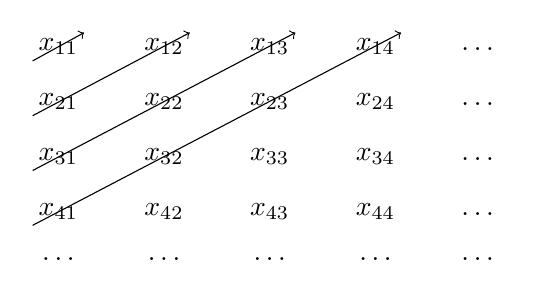
\begin{tikzpicture}
  \matrix (m) [matrix of math nodes, inner sep=2pt, row sep=1em, column sep=1em]
  {
    x_{11} && x_{12} & &x_{13} && x_{14} && \dots \\
    x_{21} & &x_{22} & &x_{23} & &x_{24}&& \dots \\
    x_{31} & &x_{32} && x_{33} && x_{34}& & \dots \\
    x_{41} & &x_{42} & &x_{43} && x_{44} && \dots \\
    \dots     & &\dots     & &\dots     & &\dots     & & \dots\\
  };
  \draw [->] (m-1-1.south west) -- (m-1-1.north east);
  \draw [->] (m-2-1.south west) -- (m-1-3.north east);
  \draw [->] (m-3-1.south west) -- (m-1-5.north east);
  \draw [->] (m-4-1.south west) -- (m-1-7.north east);
\end{tikzpicture}
\end{center}
$E_n$的元素构成了该阵列的第$n$行, 只需按箭头的顺序将该阵列的元素做成以下序列
$$x_{11}, x_{21}, x_{22},  x_{31}, x_{32}, x_{33},x_{41}, x_{42}, x_{43}, x_{44}, \cdots$$
即可得出该阵列遍历了$S$的一切元素. 倘若上述序列有重复元素, 就仅保留一个而将多余的元素剔除.

此时存在$T\subset J$, 并且可以建立一个$T$到$S$的$1-1$映射, 也即$T\sim S$. 这里的$J$为一切正整数构成的集合.

由于$T$要么是有限的, 要么是无限的, 根据定理\ref{thm:th2.1},  如果$T$是无限的, 那么$T$是可数的, 故而$T$和$S$均是至多可数的.

由于$E\subset S$, 而$E_1$是无限的, 故而$S$也是无限的, 因此$S$是可数的.


\end{proof}
\begin{corollary}
假定$A$是至多可数的, 并且对于一切$\alpha\in A$, $B_\alpha$是至多可数的. 那么
$$T=\bigcup_{\alpha\in A}B_\alpha$$
是至多可数的.
\end{corollary}

\begin{theorem}\label{thm:2.3}
  设$A$是可数集, $B_n$是一切$n$元数组$(a_1,a_2,\cdots,a_n)$构成的集合, 其中$a_k\in A\, (k=1,\cdots,n)$, 并且元素$a_1$, $a_2$, $\cdots$, $a_n$可能相同, 那么$B_n$是可数的.
\end{theorem}
\begin{proof}
  由于$B_1=A$, 故$B_1$是可数的. 假设$B_{n-1}\, (n=2,3,\cdots)$是可数的, 那么$B_{n}$的元素具有如下形式
  $$(b,a),\quad b\in B_{n-1}, a\in A$$
  对于某个固定的$b$, 元素对$(b,a)$构成的集合与$A$等价, 因而是可数的. 由于$B_{n-1}$是可数的, 由定理\ref{thm:th2.2}, $B_{n}$是可数个可数集的并, 因此也是可数的.

\end{proof}

\begin{corollary}
一切有理数的集合都是可数的.
\end{corollary}
\begin{proof}
   设$a, b \in \mathbb{Z}$, 有理数是$b/a$形状的数.

   在定理\ref{thm:2.3}中取$n=2$, 由于$\mathbb{Z}$是可数集, 故而数对$(b,a)$构成的集合是可数的, 因此全体分数$b/a$构成的集合是可数的.

\end{proof}

尽管以上论述表明了存在可数的无限集, 但并非所有无限集都是可数的, 可参考以下定理.
\begin{theorem}
设$A$是由数$0$和$1$构成的一切序列的集合, 则$A$是不可数集.
\end{theorem}
\begin{proof}
  设$E$是$A$的任意一个可数子集, 其元素为$s_1, s_2, \cdots, s_n$. 现在按以下方法构造一个序列$s$: 如果$s_n$的第$n$个数为1, 就令$s$的第$n$个数为0; 如果$s_n$的第$n$个数为0, 就令$s$的第$n$个数为1. 可得$s$与$E$中的任意一个序列至少有一位不同, 故而$s\notin E$. 由于$s\in A$, 因此$E$是$A$的真子集.

  假设$A$是可数集, 由于$A$的任意可数子集$E$是$A$的真子集, 那么$A$是它自身的真子集, 产生矛盾. 因此$A$是不可数集.

\end{proof}
\section{度量空间}
\begin{definition}\label{def:def1}
设$X$是一个集合, 它的元素叫做点, 如果对于任意的$p, q \in X$, 总存在实数$d(p,q)$与之对应, 那么它叫做从$p$到$q$的距离 (distance), 并且满足条件:
\begin{itemize}
\item 如果$p\neq q$, 那么$d(p,q)>0$, $d(p,p)=0$.

\item $d(p,q)=d(q,p)$.

\item 对于任意$r\in X$, $d(p,q)\leq d(p,r)+d(r,q)$.
\end{itemize}
就称$X$是一个度量空间 (metric space), 具有这三条性质的函数叫距离函数 (distance function)或度量 (metric).
\end{definition}

\begin{example}
对于Euclid空间$\R^k$来说, 距离定义为
$$d(x,y )=|x-y |,\quad x,y \in\R^k$$
由定理\ref{thm:th11}, 上式满足定义\ref{def:def1}的所有条件, 故$\R^k$是一个度量空间.
\end{example}
\begin{remark}
度量空间$X$的任意子集$Y$也是度量空间, 因为倘若定义\ref{def:def1}的条件对于任意$p, q, r\in X$成立时, 这些条件自然在$Y$中也成立.
\end{remark}
\begin{definition}
\begin{itemize}
\item 满足条件$a<x<b$的一切实数$x$构成的集合叫做开区间 (segment), 记作$(a,b)$.

\item 满足条件$a\leq x\leq b$的一切实数$x$构成的集合叫做闭区间 (interval), 记作$[a,b]$.
\end{itemize}
\end{definition}
有时还会遇到半开区间$[a,b)$和$(a,b]$, 第一个由满足条件$a\leq x<b$的一切实数$x$构成, 第二个由满足条件$a<x\leq b$的一切实数$x$构成.

设$a_i<b_i$, $i=1,\cdots,k$, 在$\R^k$中满足不等式$a_i\leq x_i\leq b_i$的$x=(x_1,x_2,\cdots,x_k)$构成的集合叫做一个$k$-方格 ($k$-cell), 1-方格就是闭区间, 2-方格就是闭矩形, 3-方格就是闭矩体, 等等.

设$x\in\R^k$且$r>0$. $R^k$中满足条件$|y-x|<r$ (或$|y-x|\leq r$)的一切点$y$构成的集合, 叫做以点$x$为中心, 半径为$r$的开球或闭球, 分别记作$B_r(x)$和$B_r^\ast(x)$.

集合$E\subset\R^k$是凸的 (convex), 如果
$$\lambda x+(1-\lambda)y \in E$$
对于一切$ x,y\in\R^k$且$0<\lambda<1$都成立.
\begin{theorem}
球和$k$-方格都是凸集.
\end{theorem}
\begin{proof}
  (1) 设$y, z\in B_r(x)$, 故而$|y-x|<r$且$|z-x|<r$, 又$0<\lambda<1$
  \begin{align*}
  |\lambda y +(1-\lambda) z-x|&=|\lambda(y-x)+(1-\lambda)(z-x)| \\
  &\leq\lambda|y-x|+(1-\lambda)|z-x| \\
  &<\lambda r+(1-\lambda)r=r
  \end{align*}
  因此开球$B_r(x)$是凸集, 闭球也可类似证明.

  (2) 设$x,y$位于某个$k$-方格中, 显然对每个$x_i$和$y_i$且$0<\lambda<1$都有
  $$a_i\leq \lambda x_i+(1-\lambda) y_i \leq b_i$$
  因此$k$-方格也是凸集.
\end{proof}
\begin{definition}
设$X$是一个度量空间, 下面提到的一切点和集合都理解为$X$的点和集合.
\begin{itemize}
\item 点$p$的邻域 (neighborhood)为$N_r(p)=\{q\in X|d(p,q)<r\}$, $r$叫做$N_r(p)$的半径 (radius).
\item 点$p$叫做集合$E$的极限点 (limit point), 如果对于$p$的任意邻域, 都存在异于$p$的点$q$, 使得$q\in E$.
\item 如果$p\in E$且$p$不是$E$的极限点, 那么$p$是$E$的孤立点 (isolated point).
\item $E$是闭集 (closed set), 如果$E$的每个极限点都是$E$的点.
\item 点$p$叫做$E$的内点 (interior point), 如果存在$p$的某个领域$N$, 使得$N \subset E$.
\item $E$是开集 (open set), 如果$E$的每个点都是$E$的内点.
\item $E$的补集 (complement)为$E^c=\{p\in X|p\notin E\}$.
\item $E$是完全集 (perfect set), 如果$E$是闭集, 并且$E$的每个点都是$E$的极限点.
\item $E$是有界集 (bounded set), 如果对于任意$p \in E$, 存在$q \in X$以及$M>0$, 使得$d(p,q)<M$.
\item $E$在$X$中稠密 (dense), 如果对于任意$p \in X$, $p$要么是$E$的极限点要么是$E$中的点(或者二者兼具).
\end{itemize}
\end{definition}

%\tikzset{every picture/.style={line width=0.75pt}}
%\begin{center}
%\begin{tikzpicture}
%\coordinate  (O) at (0,0);
%\draw [line width=.75pt]  plot[smooth, tension=.7] coordinates {(-4,2.5) (-3,3) (-2,2.8) (-0.8,2.5) (-0.5,1.5) (0.5,0) (0,-2)(-1.5,-2.5) (-4,-2) (-3.5,-0.5) (-5,1) (-4,2.5)};
%\draw[dashed] (-0.8,2.5) circle (1);
%\fill (-0.8,2.5) circle (1.5pt);
%\draw (-0.6,2.6) node [anchor=north west][inner sep=0.75pt]   [align=left] {$\displaystyle y$};
%\draw [dashed] (-2,-1.6) circle (.75);
%\fill (-2,-1.6) circle (1.5pt);
%\draw (-2,-1.6) node [anchor=north west][inner sep=0.75pt]   [align=left] {$\displaystyle x$};
%\draw (-2.1,0.9) node [anchor=north west][inner sep=0.75pt]   [align=left] {$\displaystyle E$};
%\end{tikzpicture}
%\end{center}

\begin{theorem}
  邻域必是开集.
\end{theorem}
\begin{proof}
  设邻域$E=N_r(p)$, 故而对于任意$q \in E$, 存在$h>0$, 使得
  $$d(p,q)=r-h$$
  设邻域$N=N_h(q)$, 那么邻域$N$内的所有点$s\in N$都满足$d(q,s)<h$, 故而
  $$d(p,s)\leq d(p,q)+d(q,s)<r-h+h=r$$
  可推知$s\in E$, $N\subset E$, 也即对于任意$q\in E$, $q$都是$E$的内点, 因此$E$是开集.
\end{proof}

\begin{theorem}\label{thm:th2.4}
  如果$p$是集合$E$的一个极限点, 那么$p$的每个邻域含有$E$的无限多个点.
\end{theorem}
\begin{proof}
  假设$p$的某个邻域$N$只含有$E$的有限多个点, 令$q_1\cdots q_n$是$N\cap E$中有限个异于$p$的点. 并且设
  $$r=\min_{1\leq m\leq n}d(p, q_m)$$
  显然$r>0$. 此时对于任意$ q\in E$, $q\notin N_r(p)$, 除非$q=p$. 这就与$p$是$E$的极限点矛盾. 因此$p$的每个邻域含有$E$的无限多个点.


\end{proof}
\begin{corollary}
有限的点集没有极限点.
\end{corollary}
从这里便可仔细区分闭集和完全集的区别. 考虑集合$A=[0,1]\cup \{2\}$, 它是闭的, 因为每个极限点都是$A$的点. 但$A$不是完全集, 因为$\{2\}$不是$A$的极限点.
\begin{example}
考虑下列$\R^2$的子集:
\begin{enumerate}[label=(\alph*)]
\item 满足条件$|z|<1$的一切复数$z$的集合;

\item 满足条件$|z|\leq1$的一切复数$z$的集合;

\item 一个有限集;

\item 一切整数的集合;

\item 由数$1/n\,(n=1,2,\cdots)$所组成的集合;

\item 一切复数的集合$\R^2$;

\item 开区间$(a,b)$.
\end{enumerate}
\end{example}

\begin{table}[!htbp]
\centering
\renewcommand{\arraystretch}{1.5}
\begin{tabular}{lcccc}
    & 闭集 & 开集 & 完全集 & 有界集 \\
(a) & 否  & 是  & 否   & 是   \\
(b) & 是  & 否  & 是   & 是   \\
(c) & 是  & 否  & 否   & 是   \\
(d) & 是  & 否  & 否   & 否   \\
(e) & 否  & 否  & 否   & 是   \\
(f) & 是  & 是  & 是   & 否   \\
(g) & 否  &    & 否   & 是
\end{tabular}
\end{table}

\begin{remark}
上述表格中, (g)的第二栏被空了起来, 这是因为如果视$(a,b)$为实数集$\R$的子集, 则它是开的, 倘若视其为复数集$\R^2$的子集, 它就不是开的. 此外, (c)中的集合有极限点$z=0$, 但该集合不包含它.
\end{remark}

\begin{theorem}[De Morgan律]
  设$\{E_\alpha\}$是若干(有限个或无限多个)集合$E_\alpha$的一个集族, 那么
  \begin{align}
  \left(\bigcup_\alpha E_\alpha\right)^c=\bigcap_\alpha E_\alpha^c \label{eq2.400} \\
  \left(\bigcap_\alpha E_\alpha\right)^c=\bigcup_\alpha E_\alpha^c \label{eq2.10}
  \end{align}
\end{theorem}
\begin{proof}
  令$A$和$B$分别表示式(\ref{eq2.400})的两端. 如果$x\in A$, 那么$x\notin \bigcup_\alpha E_\alpha$, 也即对于任意$\alpha$, 都有$x\notin E_\alpha$, 即$x \in E_\alpha^c$, 所以$ x\in\bigcap_\alpha E_\alpha^c$. 于是$A\subset B$. 如果$x\in B$, 那么对于所有的$ \alpha$都有$x\in E_\alpha^c$, 可推知$x\notin E_\alpha$. 故而对于任意$\alpha$, $ x \notin \bigcup_\alpha E_\alpha$, 反过来便能得到$ x\in \left(\bigcup_\alpha E_\alpha\right)^c$. 于是$B\subset A$. 这就证明了$A=B$.

  式(\ref{eq2.10})的证明与此类似.

\end{proof}
\begin{theorem}\label{thm:th2.3}
  $E$是开集当且仅当它的补集是闭集.
\end{theorem}
\begin{proof}
  设$E^c$是闭集. 任取$x\in E$, 则$x \notin E^c$, 因此$x$不是$E^c$的极限点. 此时存在$x$的一个邻域$N$, 使得$E^c\cap N=\emptyset$. 倘若$N\not\subset E$, 那么存在$q\in N$且$q \in E^c$, 产生矛盾, 故而$N\subset E$. 所以$x$是$E$的内点, 因为$x$是任取的, 所以$E$是开集.

  设$E$是开集. 任取$E^c$的极限点$x$, 则$x$的任意邻域都含有$E^c$的点. 倘若$x$是$E$的内点, 则存在$x$的一个邻域$N$使得$N\subset E$, 那么对于一切$x\in N$都有$x \notin E^c$, 产生矛盾. 故而$x$不是$E$的内点. 由于$E$是开的, $E$的每个点都是内点, 可推知$x\in E^c$, 因为$x$是任取的, 所以$E^c$是闭集.


\end{proof}
\begin{corollary}
$F$是闭集当且仅当它的补集是开集.
\end{corollary}
\begin{theorem}\label{thm:th2.13}
\begin{enumerate}[label=(\arabic*)]
  \item 任意一组开集$\{G_\alpha\}$的并$\bigcup_\alpha G_\alpha$是开集;

  \item 任意一组闭集$\{F_\alpha\}$的交$\bigcap_\alpha F_\alpha$是闭集;

  \item 任意一组有限个开集$G_1, G_2,\cdots, G_n$的交$\bigcap_{i=1}^nG_i$是开集;

  \item 任意一组有限个闭集$F_1, F_2,\cdots, F_n$的并$\bigcup_{i=1}^nF_i$是闭集.
\end{enumerate}
\end{theorem}
\begin{proof}
  (1) 设$G=\bigcup_\alpha G_\alpha$. 任取$x\in G$, 那么存在某个$\alpha$使得$x\in G_\alpha$, 从而$x$是$G_\alpha$的内点, 也是$G$的内点. 所以$G$是开集.

  (2) 设$F= \bigcap_\alpha F_\alpha$. 由定理\ref{thm:th2.3}得$F_\alpha^c$是开集, 由(1)可知$\bigcup_\alpha F_\alpha^c$也是开集. 根据De Morgan律可知$\left(\bigcap_\alpha F_\alpha\right)^c$是开集, 所以$F$是闭集.

  (3) 设$H=\bigcap_{i=1}^nG_i$. 由于$G_i\, (i=1,\cdots,n)$是开集, 故而对于任意$x\in H$, 存在$N_i=N_{r_i}(x)$, 使得$N_i\subset G_i$. 令
  $$r=\min(r_1,\cdots,r_n)$$
  又令$N=N_r(x)$, 于是对任意$i=1,\cdots,n$都有$N\subset G_i$, 从而$N\subset H$.

  (4) 由定理\ref{thm:th2.3}和De Morgan律即可从(3)中推得结论.


\end{proof}
\begin{remark}
 上述定理中的(3)和(4), 两个组的有限性是必不可少的: 设开区间$G_n=(-1/n,1/n)\,(n=1,2\cdots)$, 它是$\R$的开子集. 再令$G=\bigcap_{n=1}^\infty G_n$, 那么$G$仅由$x=0$这一点构成, 因而不是$\R$的开子集.

 由此可见, 一组无限多个开集的交不一定是开集, 一组无限多个闭集的并不一定是闭集.
\end{remark}
\begin{definition}
设$X$是度量空间, 如果$E\subset X$, $E'$为$E$在$X$中的所有极限点构成的集合, 那么$\overbar{E}=E\cup E'$叫做$E$的闭包 (closure).
\end{definition}
\begin{theorem}\label{thm:th2.5}
  设$X$是度量空间, $E\subset X$, 那么
  \begin{enumerate}[label=(\arabic*)]
  \item $\overbar{E}$是闭集;

  \item $E=\overbar{E}$当且仅当$E$是闭集;

  \item 如果闭集$F\subset X$且$E\subset F$, 那么$\overbar{E}\subset F$.
  \end{enumerate}
\end{theorem}
\begin{proof}
  (1) 任取$p\in X$且$p\notin \overbar{E}$,  于是$p\in\overbar{E}^c$. 可推知$p$既不是$E$的点, 也不是$E$的极限点, 故存在$p$的一个邻域$N=N_p(r)$, 使得$N\cap E=\emptyset$. 考虑邻域$N$内的某一点$q$, 满足
    $$d(p,q)=h<r$$
    其中$h$为某个正实数.

  倘若$N\not\subset\overbar{E}^c$, 必有$q\in N$且$q \notin \overbar{E}^c$,
  这也蕴含着$q \in \overbar{E}$. 由于$\overbar{E}=E\cup E'$, 那么$q \in E'$, 也即$q$是$E$的极限点. 由定理\ref{thm:th2.4}可知$q$的一个半径为$r-h$邻域$N^\ast$包含着无数个$E$的点, 并且对于任意$q^\ast\in N^\ast$, 都有$d(q,q^\ast)<r-h$, 故而
  $$d(p,q^\ast)\leq d(p,q)+d(q,q^\ast)<h+r-h=r$$
 也即$q^\ast \in N$, 可推知$N^\ast\subset N$. 然而$N\cap E=\emptyset$意味着$N^\ast\cap E=\emptyset$, 与$N^\ast$中包含着无数个$E$的点相矛盾. 这就证明了$N \subset \overbar{E}^c$, 因此$\overbar{E}^c$是开集, 也即$\overbar{E}$是闭集.

  (2) 如果$\overbar{E}=E$, 由(1)可知$\overbar{E}$是闭集, 故$E$也是闭集. 如果$E$是闭集, 那么$E$的极限点都是$E$的点, 即$E'\subset E$, 由闭包的定义可知$E=\overbar{E}$.

  (3) 由于$F$是闭集, 那么$F' \subset F$. 任取一点$x\in E'$, 则$x$是$E$的极限点, 那么对于任意邻域$N_r(x)$, 总存在$ x^\ast\neq x$, 使得$x^\ast\in E$. 因为$E\subset F$, 所以$x^\ast \in F$, 故而$x^\ast$也是$F$的极限点, 于是$x^\ast \in F'$. 因此$E' \subset F'\subset F$, 再根据$E\subset F$即可得到$\overbar{E}\subset F$.
\end{proof}
$\overbar{E}$是$X$中包含着$E$的最小闭子集, 因为$F$是任意闭集而$\overbar{E}$也是闭的且$\overbar{E}\subset F$.
\begin{theorem}\label{thm:th2.15}
  设$E$是一个非空且上有界的实数集, 令$y=\sup E$, 那么$y\in \overbar{E}$. 如果$E$是闭集, 那么$y \in E$.
\end{theorem}
\begin{proof}
  如果$y\in E$, 那么显然有$y\in\overbar{E}$. 如果$y \notin E$, 由于$y=\sup E$, 那么对于任意给定的$ \epsilon>0$, 存在点$ x\in E$, 使得$y-\epsilon<x<y$, 也即$y$的任意半径为$\epsilon$的邻域$N$中总存在异于$y$的点$x$使得$x\in E$, 因而$y$是$E$的极限点, $y\in \overbar{E}$. 如果$E$是闭集, 由定理\ref{thm:th2.5}可知$E=\overbar{E}$, 也即$y \in E$.


\end{proof}
\begin{definition}
设$X$是度量空间并且$E\subset Y\subset X$, 如果对于一切$ p\in E$, 存在$ r>0$, 使得当$d(p,q)<r$且$q\in Y$时有$q\in E$, 那么$E$关于$Y$是开的.
\end{definition}
\begin{theorem}\label{thm:th2.7}
  设$Y\subset X$, $Y$的子集$E$关于$Y$是开的, 当且仅当$X$中存在某个开子集$G$, 使得$E=Y\cap G$.
\end{theorem}
\begin{proof}
  由于$E$关于$X$是开的, 那么对于一切$ p\in E$, 存在$r_p>0$, 使得当$d(p,q)<r$且$q\in Y$时有$q\in E$. 令$V_p$为以$p$为中心, 半径为$r_p$的邻域, 并定义
  $$G=\bigcup_{p\in E}V_p$$
  由于邻域是开集并且开集的并也是开集, 因此$G$是$X$的开子集.

  因为对任意的$p\in E$都有$p \in V_p$, 并且$E$是$Y$的子集, 因此$E\subset G\cap Y$. 由于$E$关于$Y$是开的, 那么对所有的$ p\in V_p\cap Y$, 必然有$p\in E$, 也即$V_p\cap Y\subset E$, 这里$p$的选取可以使得$G\cap Y\subset E$. 如若不然, 则存在某个$p \in E$但$p\notin V_p$, 产生矛盾. 因此就得到了$E=G\cap Y$.

  反过来看, 如果$G$是$X$的一个开集并且$E=G\cap Y$, 那么对于任意$p \in E$, 总存在$ V_p\subset (G\cap Y)\subset G$, 于是$V_p\cap Y\subset E$, 因此$E$关于$Y$是开集.


\end{proof}
\begin{example}\label{ex222}
如果$E\subset Y\subset X$, 那么$E$可能关于$Y$是开的, 而关于$X$不是开的.

取$E=[0,1)$, $Y=[0,1]$, $X=\R$, 那么有$E\subset Y\subset X$. $E$关于$X$不是开的, 因为当$p=0$时, 不存在$r>0$, 使得当$|q|<r$且$q<0$. 但$E$关于$Y$是开的, 因为只需取开区间$G=(-1,1)$即有$E=G\cap Y$, 由定理\ref{thm:th2.7}即可证得.
\end{example}
\section{紧集}
\begin{definition}
设$E$是度量空间$X$的一个集合, $E$的开覆盖 (open cover)指的是$X$的一组开子集$\{G_\alpha\}$, 使得$E\subset\bigcup_\alpha G_\alpha$.
\end{definition}
\begin{definition}
度量空间$X$的子集$K$是紧的 (compact), 如果$K$的每个开覆盖总含有一个有限子覆盖. 换言之, 如果$\{G_\alpha\}$是$K$的一个开覆盖, 那么总有有限多个$\alpha_1,\cdots,\alpha_n$使得
$$K\subset G_{\alpha_1}\cup\cdots\cup G_{\alpha_n}$$
\end{definition}
\begin{example}
开区间$(0,1)$不是紧的. 这是因为存在集合$G_n=(1/n, 1)$, 使得$ \bigcup_{n=1}^\infty G_n$是$(0,1)$的一个开覆盖, 但是它没有有限子组可以盖住$(0,1)$.
\end{example}
\begin{example}
集合$K\subset\R$是由$0$和诸多$1/n\,(n=1,2,\cdots)$构成的集合, 那么$K$是紧集.

设$\{V_\alpha\}$是$K$的任意开覆盖. 因为$0\in K$, 所以对某个指标$\alpha_0$使得$0\in G_{\alpha_0}$. 因为$G_{\alpha_0}$是开的, 所以存在$0$的某个半径为$r$的邻域$V$使得$V\subset G_{\alpha_0}$.

取正整数$N$使得$\displaystyle\frac{1}{N}<r$, 因此当$n>N$时
$$\frac{1}{n}<\frac{1}{N}<r$$
从而此时$\displaystyle\frac{1}{n}\in V\subset G_{\alpha_0}$. 又设$G_{\alpha_i}$是$\displaystyle\frac{1}{i}$的开覆盖, $i=1,\cdots,N$. 于是
$$K\subset G_{\alpha_0}\cup G_{\alpha_1}\cup\cdots\cup G_{\alpha_N}$$
\end{example}
\ref{ex222}表明, 如果$E\subset Y\subset X$, 那么$E$可能关于$Y$是开的, 但关于$X$却不是. 因此, 集合的开与不开、闭与不闭全在于被安置的空间. 然而, 紧性却表现得较好.
\begin{theorem}
  设$K\subset Y\subset X$, 那么$K$关于$X$是紧的当且仅当$K$关于$Y$是紧的.
\end{theorem}
\begin{proof}
  设$K$关于$X$是紧的, 并且$\{V_\alpha\}$是$Y$的一组开子集, 使得$ K\subset\bigcup_{\alpha}V_\alpha$. 由定理\ref{thm:th2.7}可知对任意$\alpha$都存在关于$X$是开的集合$G_\alpha$, 使得$V_\alpha=Y\cap G_\alpha$. 因为$K$关于$X$是紧的, 故可以选出有限个指标$\alpha_1,\cdots,\alpha_n$, 使得
    \begin{equation}\label{eq2.8}
    K\subset G_{\alpha_1}\cup\cdots\cup G_{\alpha_n}
    \end{equation}
    又因为$K\subset Y$, 根据集合运算的分配律可知
    \begin{equation}\label{eq2.9}
    K\subset V_{\alpha_1}\cup\cdots\cup V_{\alpha_n}
    \end{equation}
    因此$K$关于$Y$是紧的.

    反过来设$K$关于$Y$是紧的. 令$\{G_\alpha\}$是$X$的一组开子集, 使得$ K\subset\bigcup_{\alpha}G_\alpha$. 因为$K$关于$Y$是紧的, 故可以选出有限个指标$\alpha_1,\cdots,\alpha_n$, 使得式(\ref{eq2.9})成立. 又因为$V_\alpha=Y\cap G_\alpha$, 故而$V_\alpha\subset G_\alpha$, 于是从式(\ref{eq2.9})中便能推知式(\ref{eq2.8})成立, 因此$K$关于$X$是紧的.
\end{proof}
按照这一定理, 在许多场合下, 可以认为紧集本身就是紧度量空间, 而不必考虑它是被安置在什么空间内的. 特别是谈论开空间或闭空间没有什么意义(每个度量空间$X$是它自身的开子集也是闭子集), 但是讨论紧度量空间却十分有意义.
\begin{theorem}\label{thm:th2.8}
  度量空间的紧子集都是闭集.
\end{theorem}
\begin{proof}
  设$K$是度量空间$X$的紧子集, 并且任取$p\in K^c$. 令$q\in K$, $V_q$和$W_q$分别是$p$和$q$的邻域, 并且它们的半径小于$\displaystyle\frac{1}{2}d(p,q)$. 因为$K$是紧的, 所以在$K$中存在有限多个$q_1,\cdots,q_n$使得
  $$K\subset W_{q_1}\cup\cdots\cup W_{q_n}=W$$
  令$V=V_{q_1}\cap\cdots\cap V_{q_n}$, 任取$\gamma\in V$, 那么对于任意$k=1,\cdots,n$都有$\gamma\in V_{q_k}$. 这也意味着$\gamma \notin W_{q_k}$, 否则就有
  \begin{align*}
  d(p_k,q_k)&\leq d(p_k,\gamma)+d(\gamma,q_k) \\
  &<\frac{1}{2}d(p_k,q_k)+\frac{1}{2}d(p_k,q_k) \\
  &=d(p_k,q_k)
  \end{align*}
  产生矛盾. 也即对任意$k=1,\cdots,n$, $\gamma\notin W_{q_k}$, 进而$\gamma\notin W$. 这就证明了$V\cap W=\emptyset$, 并且$V\subset W^c$. 由于$W$将$K$覆盖住了, 那么有$W^c\subset K^c$, 因此得到$V\subset K^c$, 也即$p$是$K^c$的内点. 由于$p$是任取的, 故$K^c$是开集, 也就证明了$K$是闭集.
\end{proof}
\begin{theorem}\label{thm:th2.18}
  紧集的闭子集都是紧集.
\end{theorem}
\begin{proof}
  设$F\subset K\subset X$, $F$是闭的而$K$是紧的. 令$\{V_\alpha\}$是$F$的一个开覆盖, 将$F^c$加入$\{V_\alpha\}$后便能得到一个$K$的开覆盖$\Omega$(单凭$\{V_\alpha\}$不一定能盖住$K$). 因为$K$是紧的, 那么$\Omega$的一个有限子组$\Phi$也能盖住$K$, 从而也能盖住$F$. 如果$F^c$位于$\Phi$中, 那便将其去掉, 剩下的仍是$F$的一个有限子覆盖, 因此$F$是紧的.
\end{proof}
\begin{corollary}\label{cor:cor2.1}
如果$F$是闭的而$K$是紧的, 那么$F\cap K$是紧的.
\end{corollary}
\begin{proof}
  由于$K$在度量空间中是紧的, 则它是闭的. 因为$F$是闭的, 所以$F\cap K$也是闭的. 由定理\ref{thm:th2.8}可得, $F\cap K\subset K$也是紧的.
\end{proof}
\begin{theorem}\label{thm:th2.14}
  如果$\{K_\alpha\}$是度量空间$X$的一组紧子集, 并且$\{K_\alpha\}$中任意有限个集合的交都不是空集, 那么$\bigcap K_\alpha$也不是空集.
\end{theorem}
\begin{proof}
  利用反证法. 假设$\cap K_\alpha$是空集, 取$\{K_\alpha\}$的一个集合$K_1$, 则$K_1$中不存在同时属于每个$K_\alpha$的点. 令$G_\alpha=K_\alpha^c$, 那么$\{G_\alpha\}$便形成$K_1$的一个开覆盖. 因为$K_1$是紧的, 所以存在有限个指标$\alpha_1,\cdots,\alpha_n$, 使得$K_1\subset G_{\alpha_1}\cup\cdots\cup G_{\alpha_n}$. 注意到$G_\alpha=K_\alpha^c$, 利用De Morgan律可得
  $$K_1\cap K_{\alpha_1}\cap\cdots\cap K_{\alpha_n}=\emptyset$$
  与题设相矛盾. 因此$\bigcap K_\alpha$不是空集.


\end{proof}
\begin{corollary}\label{cor:cor1}
设$\{K_n\}$是非空紧集的序列并且$K_{n+1}\subset K_n\,(n=1,2\cdots)$, 那么$ \bigcap_{n=1}^\infty K_n$是非空的.
\end{corollary}
\begin{theorem}\label{thm:th2.9}
  设$E$是紧集$K$的无限子集, 那么$E$在$K$中有极限点.
\end{theorem}
\begin{proof}
  假设$E$在$K$中没有极限点, 那么对于任意$q\in K$, 存在$V_q$使得它最多只含有$E$的一个点(如果$q\in E$, 那这点就是$q$). 由此推知不存在$\{V_q\}$的有限子组可以覆盖$E$, 由于$E\subset K$, 那么也不能盖住$K$, 与$K$是紧集矛盾. 因此$E$在$K$中必有极限点.
\end{proof}
\begin{remark}
紧集要求它的任意开覆盖都存在一个有限子覆盖可以盖住它.
\end{remark}
\begin{theorem}[Cantor闭区间套定理]\label{thm:th2.10}
  设$\{I_k\}$是$\R$中的闭区间序列, 并且$I_{n+1}\subset I_n\,(n=1,2,\cdots)$, 那么$ \bigcap_{n=1}^\infty I_n$非空.
\end{theorem}
\begin{proof}
  设$I_n=[a_n,b_n]$, 令$E$是一切$a_n$构成的集合. 由于$I_{n+1}\subset I_n$, $b_1$是$E$的一个上界, 故而$E$有上确界, 记为$x=\sup E$. 令$m$和$n$都是正整数, 使得
  $$a_n\leq a_{m+n}\leq b_{m+n}\leq b_m$$
  于是对任意$m=1,2,\cdots$都有$x\leq b_m$, 又因为$a_m\leq x$, 所以$x\in I_m$, 也即$x\in \bigcap_{m=1}^\infty I_m$.
\end{proof}
\begin{theorem}\label{thm:th2.11}
  设$k$是正整数. 如果$\{I_n\}$是$k$-方格构成的序列, 并且$I_{n+1}\subset I_n\,(n=1,2,\cdots)$, 那么$ \bigcap_{n=1}^\infty I_n$非空.
\end{theorem}
\begin{proof}
  设$I_n$由一切满足条件
  $$a_{n,j}\leq x_j \leq b_{n,j}\quad (1\leq j\leq k;\,\,n=1,2,\cdots)$$
  的点$x=(x_1,x_2,\cdots,x_k)$组成. 设闭区间$I_{n,j}=[a_{n,j},b_{n,j}]$, 由定理\ref{thm:th2.10}, 对于一切$1\leq j \leq k$,  总存在$x_j^\ast \in \R$使得
  $$a_{n,j}\leq x^\ast_j\leq b_{n,j}\quad (1\leq j\leq k;\,\,n=1,2,\cdots)$$
  取$x^\ast=(x_1^\ast,x_2^\ast,\cdots,x_j^\ast)$, 那么$x^\ast\in I_n$, 从而$ \bigcap_{n=1}^\infty I_n$非空.
\end{proof}
\begin{theorem}\label{thm:th2.12}
  每个$k$-方格都是紧集.
\end{theorem}
\begin{proof}
  设$I$是$k$-方格, 它由一切满足条件$a_j\leq x_j\leq b_j\,(1\leq j \leq k)$的点$x=(x_1,\cdots,x_k)$构成. 令
  $$\delta=\begin{bmatrix}
\displaystyle\sum_{j=1}^{k}(b_j-a_j)^2
\end{bmatrix}^{\frac{1}{2}} $$
  如果$x, y \in I$, 显然有$|x-y |\leq \delta$.

  假设存在$I$的一个开覆盖$\{G_\alpha\}$, 它的任意有限子组都不能盖住$I$. 令$c_j=(a_j+b_j)/2$, 那么闭区间$[a_j,c_j]$和$[c_j,b_j]$可以确定$2^k$个$k$-方格$Q_i$, 它们的并就是$I$. 于是$Q_i$中至少存在某个$k$-方格$I_1$不能被$\{G_\alpha\}$的任何有限子组盖住, 否则$I$也会被$\{G_\alpha\}$的有限子组盖住.

  按照此种方式继续将$I_1$分划, 可以得到一个序列$\{I_n\}$, 并且满足以下性质:

  (a) $I\supset I_1\supset I_2\supset \cdots$;

  (b) $I_n$不能被$\{G_\alpha\}$有限子组覆盖;

  (c) 如果$x,y \in I_n$, 那么$|x-y |\leq 2^{-n}\delta$.

  \noindent 由(a)和定理\ref{thm:th2.11}可知存在一点$\bx$位于每个$I_n$之内. 因为$\{G_\alpha\}$是$I$的开覆盖, 所以存在某个指标$\alpha$使得$x^\ast\in G_\alpha$.

  由于$G_\alpha$是开的, 故存在$r>0$, 使得当$|y-x^\ast|<r$时有$y \in G_\alpha$. 利用实数的Archimedes性质, 可知必存在正整数$N$使得$2^{-N}\delta<r$, 由此可推知必有$y \in G_\alpha$, 于是$I_n\subset G_\alpha$, 与(b)矛盾. 所以$k$-方格是紧集.

\end{proof}

\begin{theorem}\label{thm:th2.16}
  如果$\R^k$中的一个集合具有下列三个性质之一, 那么它也具有其他两个性质:
  \begin{enumerate}[label=(\arabic*)]
  \item $E$是闭的且有界;

  \item $E$是紧的;

  \item $E$的每个无限子集在$E$内有极限点.
  \end{enumerate}
\end{theorem}
\begin{proof}
  如果(1)成立, 那么存在某个$k$-方格$I$使得$E\subset I$, 由于$k$-方格是紧的且紧集的闭子集也是紧集, 因此(2)成立.

  如果(2)成立, 那么(c)是定理\ref{thm:th2.9}的直接结论.

  如果(3)成立, 假设$E$不是有界的, 那么$E$中存在点$x$满足
  $$|x_n|=n+1>n\,(n=1,2\cdots)$$
  由这些$x_n$构成的集合是$E$的无限子集, 并且在$\R^k$中没有极限点, 那么在$E$中也没有极限点, 产生矛盾. 因此$E$是有界的.

  假设$E$不是闭的, 那么存在某个极限点$x_0\in \R^K$且$x_0\notin E$. 对于每个$n=1,2,\cdots$总能找到$x_n$满足$|x_n-x_0|<\displaystyle \frac{1}{n}$. 令$S$是这些$x_n$构成的集合, 显然$S$是无限集, 现在来证明$x_0$是$S$在$\R^k$中唯一的极限点.

  因为对于任意$x_0$的任意半径为$r$的邻域, 总存在点$x^\ast$, 使得$\displaystyle |x^\ast-x_0|<1/n<r$, 这可以由实数的
  Archimedes性质保证, 因而$x_0$是$S$的极限点. 假设除了$x_0$之外, $S$还有极限点$y \in \R^k$, 那么除了有限的几个$n$外, 对于其余的$n$都有
  \begin{align*}
  |x_n-y |&\geq |x_0-y |-|x_n-x_0| \\
  &\geq|x_0-y |-\frac{1}{n}\geq\frac{1}{2}|x_0-y|
  \end{align*}
  也就是说, 除了有限的几个点落入$y$的某一邻域内, 其余点都在邻域外, 与定理\ref{thm:th2.4}矛盾, 因此$y$必然不是$S$的极限点.

  于是$S$在$\R^k$中没有$x_0$以外的极限点, 而$x_0\notin E$, 那么$S$在$E$中也没有极限点, 与(3)的条件矛盾. 因此$E$是闭的.


\end{proof}
\begin{remark}
上述定理中(1)和(2)的等价性称为Heine-Borel有限覆盖定理, 在$\R^k$上成立, 而(2)和(3)在任何度量空间中都是等价的, (1)一般不能推出(2)和(3), 例如Lebesgue可积函数类$\mathscr{L}^2$.
\end{remark}
\begin{example}
区间$[0,\infty)$是$\R$的无界闭集, 因而不是紧的.
\end{example}
\begin{theorem}[Weierstrass定理]\label{thm:th2.17}
  $\R^k$中的每个有界无限子集在$\R^k$中都有极限点.
\end{theorem}
\begin{proof}
  设$E\subset\R^k$, 由于它是有界的, 那么必是$k$-方格$I$的一个子集. 因为$k$-方格是紧的, 由定理\ref{thm:th2.9}可知$E$在$I$中有极限点, 从而在$\R^k$中也有极限点.

\end{proof}

\section{完全集}
\begin{theorem}
  令$P$是$\R^k$中的非空完全集, 那么$P$是不可数的.
\end{theorem}
\begin{proof}
  由于$P$中存在极限点, 由定理\ref{thm:th2.4}可知$P$是无限集.

  假设$P$是可数的, 将$P$的点记作$\bx_1,\bx_2,\cdots$. 设$V_1$是$\bx_1$的任意一个邻域, 不妨令$V_1$为一切满足$|\y -\bx_1|<r$的$\y \in \R^k$构成, 那么$V_1$的闭包$\overbar{V}_1$就是由一切满足$|\y -\bx_1|\leq r$的$\y \in\R^k$构成.

  假定已经作出了邻域$V_n$, 由于$\bx_n$是极限点, 由定理\ref{thm:th2.4}可知$V_n\cap P\neq\emptyset$, 并且存在$\bx_{n+1} \in V_n$, 由于$V_n$是开的, 那么存在$\bx_ {n+1}$的邻域使得$\overbar{V}_{n+1}\subset V_n$. 进一步, 还可以调整$V_n$和$V_{n+1}$的半径$\delta_1$和$\delta_2$, 使得当
  $$\delta_2<\min\{|\bx_n-\bx_{n+1}|,\delta_1- |\bx_n-\bx_{n+1}|\}$$
  成立时还能同时满足$\overbar{V}_{n+1}\subset V_n$和$\bx_n\notin \overbar{V}_{n+1}$. 再次,  由定理\ref{thm:th2.4}可知$V_{n+1}\cap P$也是非空的. 由数学归纳法, 我们便可构造出满足以下三条性质的一组领域序列$\{V_\alpha\}$:

  (a) $\overbar{V}_{n+1}\subset V_n$;

  (b) $x_n\notin \overbar{V}_{n+1}$;

  (c) $V_{n+1}\cap P\neq\emptyset$.

\noindent 其中$n=1,2,\cdots$.

  令$K_n=\overbar{V}_{n}\cap P$. 因为$\overbar{V}_n$是$\R^k$内的有界闭集, 由Heine-Borel定理可知$\overbar{V}_n$是紧集. 因为$x_n\notin K_{n+1}$, 所以$ \bigcap_{n=1}^\infty K_n$中没有$P$的点. 这样一来, $K_n\subset P$就意味着$ \bigcap_{n=1}^\infty K_n$是空集, 但是由(c)来看, 每个$K_n$均不是空集, 产生矛盾. 因此$P$是不可数的.

\end{proof}
\begin{corollary}
每个闭区间$[a,b]\,(a<b)$是不可数的. 特别地, 一切实数集都是不可数的.
\end{corollary}
\begin{example}[$\,$(Cantor集)]
Cantor集表明, 在$\R$中确有不包含开区间的完全集.

令$E_0$是闭区间$[0,1]$, 显然它是紧的. 去掉开区间$(1/3,2/3)$, 并令$E_1$是闭区间
$$\left[0,\frac{1}{3}\right],\quad\left[\frac{2}{3},1\right]$$
的并. 再将这两个闭区间都三等分, 并去掉中间的那个开区间. 令$E_2$是闭区间
$$\left[0,\frac{1}{9}\right],\quad\left[\frac{2}{9},\frac{3}{9}\right],\quad\left[\frac{6}{9},\frac{7}{9}\right],\quad\left[\frac{8}{9},1\right]$$
的并. 按照这个方式进行下去, 就得到一个紧集序列$\{E_n\}$, 显然有
\begin{itemize}
\item $E_1\supset E_2\supset E_3\supset \cdots$;

\item $E_n$是$2^n$个闭区间的并, 每个闭区间的长度为$3^{-n}$.
\end{itemize}
那么集合
$$P=\bigcap_{n=1}^\infty E_n$$
叫做Cantor集. 由定理\ref{thm:th2.13}可知$P$是闭集, 由于$P\subset E_0$, 那么$P$是有界的, 所以$P$是紧的, 再由定理\ref{thm:th2.14}可知$P$非空, 它的示意图如下.

\begin{center}
\genpic{\linewidth}{6}
\end{center}


如果$k$和$m$都是正整数, 那么没有一个形式为
\begin{equation}\label{eq2.11}
\left(\frac{3k+1}{3^m},\frac{3k+2}{3^m}\right)
\end{equation}
的开区间能够和$P$有公共点. 因为对于每个开区间$(\alpha,\beta)\subset (0,1)$都存在(\ref{eq2.11})那样的子集, 只要满足
$$3^{-m}<\frac{\beta-\alpha}{4}$$
因此开区间都在Cantor集的构建过程中被剔除了, 也即$P$不能含有任意开区间.

设$x\in P$, 而$S$是包含$x$的任意一个开区间. 令$I_n$是$E_n$中包含$x$的那个闭区间, 那么存在充分大的正整数$n$使得$I_n\subset S$, 再设$x_n$为$I_n$的一个不等于$x$的端点. 从构造$P$的方法可知$x_n\in P$, $x$是$P$的极限点, 于是$P$是完全集且不包括任何开区间.
\end{example}

Cantor集的一个有趣的性质是, 它提供了一个Lebesgue测度为0的不可数集的例子.
\section{连通集}
\begin{definition}
设$A$, $B$是度量空间$X$的两个子集. 如果$A\cap\overbar{B}$及$\overbar{A}\cap B$都是空集, 即$A$的点不在$B$的闭包中, $B$的点也不在$A$的闭包中, 那么$A$和$B$是分离的 (separated).

如果$E\subset X$不是两个非空分离集的并, 则称$E$是连通集 (connected set).
\end{definition}
\begin{remark}
分离的两个集不相交, 但不相交的两个集未必分离. 例如闭区间$[0,1]$和开区间$(1,2)$不相交也不分离, 因为$1$是$(1,2)$的极限点. 但是, 开区间$(0,1)$和$(1,2)$是分离的.
\end{remark}
\begin{theorem}\label{thm:th2.19}
  $\R$的子集$E$是连通的, 当且仅当如果$x,y\in E$, 并且$x<z<y$时有$z\in E$.
\end{theorem}
\begin{proof}
  给定$\R$的连通子集$E$. 令$x,y\in E$, 假设存在$z\in (x,y)$且$z\notin E$, 那么$E=A_z\cup B_z$, 其中
  $$A_z=E\cap (-\infty,z),\quad B_z=E\cap(z,\infty)$$
  因为$x\in A_z$, $y\in B_z$, 所以$A_z$和$B_z$非空. 又因为$A_z\subset(-\infty,z)$, $B_z\subset(z,\infty)$, 所以$A_z$和$B_z$是分离的, 这意味着$E$不是连通的, 产生矛盾. 因此$z\in E$.

  反过来看, 令$x,y\in E$, 并且对任意$x<z<y$都有$z\in E$. 假设$E$不是连通的, 那么$E$就是两个非空分离集的并$A\cup B$. 由与$x,y\in E$, 不妨取$x\in A$而$y \in B$, 并且设$x<y$. 由于$x$和$y$是任意的, 因此$A$有上界, 它的子集$A\cap[x,y]$也有上界. 定义
  $$z=\sup\, (A\cap [x,y])$$
  由定理\ref{thm:th2.15}可知$z\in \overbar{A}$并且$z\notin B$, 特别地有$x\leq z<y$.

  如果$z\notin A$, 由$z\notin B$可知$z\notin E$, 产生矛盾; 如果$z\in A$, 由于$E$不连通, 那么$z\notin \overbar{B}$. 由实数的稠密性可知存在$z_1$使得$z<z_1<y$且$z_1\notin B$, 因此$z_1\notin E$, 产生矛盾, 这就说明$E$必是连通集.


\end{proof}
\chapter{序列与级数}
\section{收敛序列}
\begin{definition}
\begin{itemize}
\item 度量空间$X$中的序列$\{p_n\}$是收敛的 (convergent), 如果存在一个具有以下性质的点$p\in X$: 对于任意$\epsilon>0$, 存在一个正整数$N$, 使得当$n\geq N$时有$d(p_n,p)<\epsilon$.

\item 如果$\{p_n\}$收敛于$p$, 则称$p$是$\{p_n\}$的极限 (limit), 记作$p_n\rightarrow p$, 或者
$$\limn  p_n=p$$
如果$\{p_n\}$不收敛, 那么它就发散 (diverge).
\end{itemize}
\end{definition}

\begin{remark}
收敛序列的定义取决于度量空间$X$而非$\{p_n\}$. 例如序列$\{1/n\}$在$\R$中收敛于0, 而在一切正实数集中不收敛, 因为$0$不是正实数, 即$0\not\in X=(0,\infty)$.
\end{remark}

\begin{theorem}[迫敛定理]
设实数序列$\{x_n\}$, $\{y_n\}$和$\{z_n\}$满足$x_n\leq y_n\leq z_n$, 并且
$$\limn x_n=\limn z_n=l$$
那么$$\limn y_n=l$$
\end{theorem}
\begin{proof}
  任取$\epsilon>0$, 选取某个充分大的正整数$N$使得当$n>N$时有
  $$|x_n-l|<\frac{\epsilon}{4}, \quad |z_n-l|<\frac{\epsilon}{4}$$
  由三角不等式可知
  $$|x_n-z_n|\leq |x_n-l|+|z_n-l|<\frac{\epsilon}{2}$$
  由于$x_n\leq y_n\leq z_n$, 故而
  $$|y_n-x_n|=y_n-x_n \leq z_n-x_n=|z_n-x_n|$$
  再次利用三角不等式可知
  $$|y_n-l|\leq |y_n-x_n|+|x_n-l|\leq |z_n-x_n|+|x_n-l|<\frac{3\epsilon}{4}$$
\end{proof}

\begin{definition}
一切点$p_n\,(n=1,2,\cdots)$的集合是$\{p_n\}$的值域, 序列的值域可以是有限的也可以是无限的. 如果是有限的, 那么$\{p_n\}$是有界的.
\end{definition}
\begin{example}
考虑以下的复数序列(即$X=\R^2$):
\begin{enumerate}[label=(\alph*)]
\item 如果$s_n=1/n$, 那么$\displaystyle\limn  s_n=0$. 值域是无限的, 但序列是有界的;

\item 如果$s_n=n^2$, 那么$\{s_n$\}发散. 值域是无限的, 序列也是无界的;

\item 如果$s_n=1+[(-1)^n/n]$, 那么$\{s_n\}$收敛于1. 有界且值域是无限的;

\item 如果$s_n=\text{i}^n$, 那么$\{s_n\}$发散. 有界且值域是有限的;

\item 如果$s_n=1$, 那么$\{s_n\}$收敛于1. 有界且值域是有限的.
\end{enumerate}
\end{example}
\begin{theorem}\label{thm:th3.5}
  设$\{p_n\}$为度量空间$X$中的序列, 那么
  \begin{enumerate}[label=(\arabic*)]
  \item $\{p_n\}$收敛于$p\in X$, 当且仅当$p$的每一个邻域, 都可以包含$\{p_n\}$的除有限项以外的一切项;

  \item 如果$p\in X$且$p'\in X$, 如果$\{p_n\}$既收敛于$p$又收敛于$p'$, 那么$p=p'$;

  \item 如果$\{p_n\}$收敛, 那么$\{p_n\}$有界;

  \item 如果$E\subset X$且$p$是$E$的极限点, 那么$E$中存在一个序列$\{p_n\}$, 使得$ p=\limn  p_n$;

  \item 如果$E\subset X$, 每个$p_n$都在$E$内并且$p_n\rightarrow p$, 那么$p\in \overbar{E}$.
  \end{enumerate}
  \end{theorem}
  \begin{proof}
    (1) 设$V$为$p\in X$的任意一个邻域, 那么对于任意$\epsilon>0$, 条件$d(p,q)<\epsilon$以及$q\in X$就意味着$q\in V$. 如果$p_n\rightarrow p$, 那么对应着这个$\epsilon$, 总能找到正整数$N$, 使得当$n\geq N$时就有$d(p_n,p)<\epsilon$. 因此当$n\geq N$时可推知$p_n\in V$.

    反过来看, 假定$p\in X$的每个邻域, 除有限个点外, 包含着其余一切点$p_n$. 任取$\epsilon>0$, 设$V$是满足$d(p,q)<\epsilon$的$q\in X$构成的集合. 根据假定, 存在正整数$N$, 使得当$n\geq N$时就有$p_n\in V$. 因此当$n\geq N$时就能得到$d(p,p_n)<\epsilon$, 所以$p_n\rightarrow p$.

    (2) 任取$\epsilon>0$, 那么存在正整数$N$和$N'$, 使得
    $$n\geq N\Rightarrow d(p_n,p)<\frac{\epsilon}{2}$$
    $$n\geq N'\Rightarrow d(p_n,p')<\frac{\epsilon}{2}$$
    因此当$n\geq \max\{N,N'\}$时就有
    $$d(p,p')\leq d(p,p_n)+d(p_n,p')<\epsilon$$
    由于$\epsilon$是任意正实数, 因此$d(p,p')=0$, 也即$p=p'$.

   (3) 如果$p_n\rightarrow p$, 那么存在正整数$N$, 使得当$n>N$时就有$d(p_n,p)<1$. 令
   $$r=\max\{1,d(p_1,p),d(p_2,p),\cdots,d(p_N,p)\}$$
   于是当$n=1,2,\cdots,N$时就有$d(p_n,p)\leq r$, 因此$\{p_n\}$是有界的.

   (4) 因为$p$是$E$的极限点, 故对于任意正整数$n$, 存在$p_n\in E$使得$\displaystyle d(p,p_n)<\frac{1}{n}$. 任取$\epsilon>0$, 存在正整数$N=\left\lfloor 1/\epsilon \right\rfloor+1$, 当$n>N$时就有$d(p_n,p)<\epsilon$, 因此$p_n\rightarrow p$.

   (5) $p$要么在$E$内要么不在$E$内. 若$p\notin E$, 由于$p_n\rightarrow p$, 则对于任意$\epsilon>0$, 总存在正整数$N$, 使得当$n\geq N$时有
   $$d(p,p_n)<\epsilon$$
   也即$p$的任意一个邻域都含有点$p_n\in E$且$p\neq p_n$, 故$p$是$E$的极限点. 因此$p\in \overbar{E}$.

  \end{proof}


  \begin{theorem}\label{thm:th3.1}
    假定$\{s_n\}$和$\{t_n\}$是复数序列, 并且$\limn  s_n=s$, $\limn  t_n=t$. 那么:
    \begin{enumerate}[label=(\arabic*)]
    \item 对于任何复数$c$, $\limn  cs_n=cs$, $\limn (c+s_n)=c+s$;

    \item $\limn (s_n+t_n)=s+t$;

    \item $\limn  s_nt_n=st$;

    \item 如果对于任意$n\ge1$都有$s_n\neq 0$且$s\neq0$, 那么$\limn 1/s_n=1/s$.
    \end{enumerate}
  \end{theorem}
  \begin{proof}
    (1) 由于$s_n\rightarrow s$, 当$c=0$时显然成立. 当$c\neq 0$时, 任取$\epsilon>0$, 存在正整数$N$, 使得当$n\geq N$时有
    $$|cs_n-cs|=|c||s_n-s|<|c|\epsilon$$
    以及
    $$|(c+s_n)-(c+s)|=|s_n-s|<\epsilon$$
    这就证明了(1).

    (2) 同样地, 任取$\epsilon>0$, 存在正整数$N_1$和$N_2$, 使得
    \begin{align*}
    &n\geq N_1\Rightarrow |s_n-s|<\frac{\epsilon}{2} \\
    &n\geq N_2\Rightarrow |t_n-t|<\frac{\epsilon}{2}
    \end{align*}
    取$N=\max\{N_1,N_2\}$, 当$n\geq N$时有
    $$|(s_n+t_n)-(s+t)|\leq |s_n-s|+|t_n-t|<\epsilon$$
    从而$\displaystyle\limn (s_n+t_n)=s+t$成立.

    (3) 由于$s_n\rightarrow s$, 那么$\{s_n\}$有界, 存在正数$X>0$使得$|s_n|<X$. 于是任取$\epsilon>0$, 总存在正整数$N$, 使得当$n\geq N$时有
    $$|s_nt_n-st|=|s_n(t_n-t)+t(s_n-s)|<(X+|t|)\epsilon$$
    因此(3)也对.

    (4) 取正整数$N_1$, 使得当$n\geq N_1$时有$|s_n-s|<|s|/2$, 由三角不等式
    $$|s|=|(s-s_n)+s_n|\leq |s-s_n|+|s_n|$$
    可知
    $$|s_n|>\frac{1}{2}|s|\Leftrightarrow\frac{1}{|s_n|}<\frac{2}{|s|}\quad(n\geq N_1)$$
    由于$s_n\rightarrow s$, 那么任取$\epsilon>0$, 存在正整数$N$, 使得当$n\geq N$时就有
    $$|s_n-s|<\frac{1}{2}|s|^2\epsilon$$
    于是
    $$\left|\frac{1}{s_n}-\frac{1}{s}\right|=\left|\frac{s_n-s}{ss_n}\right|<\frac{|s|}{2|s_n|}\epsilon<\epsilon$$
    由此(4)成立.
  \end{proof}
\begin{theorem}
  \begin{enumerate}[label=(\arabic*)]
  \item 设$\bx_n\in\R^k\,(n=1,2,\cdots)$并且
  $$\bx_n=(\alpha_{1,n},\cdots,\alpha_{k,n})$$
  那么序列$\{x_n\}$收敛于$\bx=(\alpha_1,\cdots,\alpha_k)$, 当且仅当
  \begin{equation}\label{eq3.1}
  \limn \alpha_{j,n}=\alpha_j\quad(1\leq j\leq k)
  \end{equation}

  \item 设$\{\bx_n\}$和$\{\y _n\}$是$\R^k$中的序列, $\{\beta_n\}$是实数序列, 且$\bx_n\rightarrow \bx$, $\y _n\rightarrow\y $, $\beta_n\rightarrow\beta$. 那么
  $$\limn (\bx_n+\y _n)=\bx+\y ,\quad \limn \bx_n\cdot\y _n=\bx\cdot\y ,\quad\limn \beta_n\bx_n=\beta\bx$$
  \end{enumerate}
\end{theorem}
\begin{proof}
   (1) 如果$\bx\rightarrow\bx$, 那么任取$\epsilon>0$, 存在正整数$N$, 使得当$n\geq N$时有
  $|\alpha_{j,n}-\alpha_j|\leq|\bx_n-\bx|<\epsilon$
  其中, 第一个不等号是由范数的定义保证的.

  反过来, 如果式(\ref{eq3.1})成立. 任取$\epsilon>0$, 存在正整数$N$, 使得当$n\geq N$时有
  $$|\alpha_{j,n}-\alpha_j|<\frac{\epsilon}{\sqrt{k}}\quad (1\leq j\leq k)$$
  也即
  $$|\bx_n-\bx|=\begin{bmatrix}
                      \displaystyle\sum_{j=1}^{k}|\alpha_{j,n}-\alpha_n|^2
                    \end{bmatrix}^{\frac{1}{2}}<\epsilon
  $$
  因此有$\bx_n\rightarrow\bx$.

  (2) 由(1)和定理\ref{thm:th3.1}可知成立.
\end{proof}
定理\ref{thm:th3.5}(3)表明, 收敛序列都是有界的. 但是反过来, $\R^k$中的有界数列并不一定收敛, 但$\R$中的单调有界数列却必然收敛.
\begin{definition}
设$n=1,2,\cdots$, 称实数序列$\{s_n\}$是
\begin{itemize}
\item 单调递增的, 如果$s_n\leq s_{n+1}$;

\item 单调递减的, 如果$s_n\geq s_{n+1}$.
\end{itemize}
\end{definition}
\begin{theorem}[单调有界收敛定理]\label{thm:th3.6}
  单调序列$\{s_n\}$是收敛的, 当且仅当它是有界的.
\end{theorem}
\begin{proof}
  假定$s_n\leq s_{n+1}$(单调递减序列证明类似), 设$E$是$\{s_n\}$的值域, 如果$\{s_n\}$是有界的, 那么$E$必有上确界$s=\sup E$, 那么
  $$s_n\leq s,\quad n=1,2,\cdots$$
  任取$\epsilon>0$, 必定存在某个正整数$N$, 使得$s-\epsilon<s_N\leq s$, 否则$s-\epsilon$是$E$的上界, 产生矛盾. 因为$\{s_n\}$是单调递增的, 那么当$n\geq N$时有
  $$s-\epsilon<s_n\leq s$$
  也即$|s_n-s|<\epsilon$, 因此$\{s_n\}$收敛于$s$.

  反过来, 如果$\{s_n\}$收敛于$s$, 那么由定理\ref{thm:th3.5}(3)可知它是有界的.

\end{proof}

\begin{example}
设实数$|C|<1$, 证明$\limn C^n=0$.
\end{example}
\begin{proof}
  如果$C=0$, 结论是显然的. 假设$0<C<1$, 那么$\{C^n\}$是单调有下界的数列, 因此必有极限$\limn C^n=L$, 注意到
  $$C^{n+1}=CC^n$$
  两端取极限得$L=CL$, 故而$L=0$. 如果$-1<-C<0$, 那么$(-C)^n=(-1)^nC^n$, 因为$\{(-1)^n\}$是有界的, 而$C^n\to0$, 故而$\limn (-C)^n=0$.
\end{proof}

\begin{example}
设$0<\alpha<1$, 证明$\limn [(n+1)^\alpha-n^\alpha]=0$.
\end{example}
\begin{proof}
  当$n\ge1$时有
  \begin{align*}
  0<(n+1)^\alpha-n^\alpha&=n^\alpha\left[\left(1+\frac{1}{n}\right)^\alpha-1\right] \\
  &\leq n^\alpha\left[\left(1+\frac{1}{n}\right)-1\right]=\frac{1}{n^{1-\alpha}}
  \end{align*}
  根据迫敛定理即可得到结论.
\end{proof}

\begin{example}
设$S$是$\R$中上有界的非空子集, $s=\sup S$, 证明在$S$中存在收敛于$s$的数列$\{x_n\}$.
\end{example}
\begin{proof}
  根据上确界的定义, 任取$\epsilon>0$, 存在$x\in S$使得
  $$s-\epsilon<x\leq s$$
  于是对于任意$n\ge1$, 存在$x_n\in S$使得
  $$s-\frac{1}{n}<x\leq s$$
  由于$\{1/n\}$趋近于0, 存在正整数$N$, 使得当$n>N$时有$n^{-1}<\epsilon$, 从而
  $$s-\epsilon<s-\frac{1}{n}<x_n\leq s<s+\epsilon$$
  也即$|x_n-s|<\epsilon$.
\end{proof}

\begin{example}[$\,$Cesaro均值]
设数列$\{x_n\}$的极限为$l$, 证明
$$\limn \frac{x_1+\cdots+x_n}{n}=l$$
\end{example}
\begin{proof}
  令$M=\sup_{n\in\mathbb{N}}|x_n-x|$, 任取$0<\epsilon<M$, 故而
  $$\left|\frac{x_1+\cdots+x_n}{n}-l\right|\leq \left|\frac{|x_1-l|+\cdots+|x_n-l|}{n}\right|\leq M$$
  根据极限的定义可知, 存在正整数$N_1$, 使得当$n>N_1$时有$|x_n-l|<\epsilon/2$, 于是
  $$\left|\frac{|x_1-l|+\cdots+|x_{N_1}-l|+\cdots+|x_n-l|}{n}\right|\leq \left|\frac{N_1M+(n-N_1)\epsilon/2}{n}\right|$$
  再取某个充分大的正整数$N_2$, 使得当$n>N_2$时有
  $$0<\frac{N_1(M-\epsilon/2)}{n}<\frac{\epsilon}{2}$$
  因此
  $$\left|\frac{x_1+\cdots+x_n}{n}-l\right|\leq \left|\frac{N_1(M-\epsilon/2)}{n}+\frac{\epsilon}{2}\right|<\epsilon$$
  取$N=\max\{N_1,N_2\}$即可完成证明.
\end{proof}

\begin{example}
设实数序列$\{x_n\}$的第一项为$\sqrt{2}$, 且满足$x_{n+1}=\sqrt{x_n+2}$, 证明极限$\limn x_n$存在.
\end{example}
\begin{proof}
  当$n=1$时, $x_1=\sqrt{2}<2$. 假设当$n=k$时也有$x_k<2$, 那么
  $$x_{k+1}=\sqrt{x_k+2}<\sqrt{2+2}=2$$
  因此对于任意正整数$n$都有$0<x_n<2$. 又因为
  $$x_{n+1}-x_n=\frac{2}{\sqrt{x_n+2}+x_n}>0$$
  所以$\{x_n\}$是单调有界的, 根据定理\ref{thm:th3.6}可知极限存在.
\end{proof}

\section{子序列}
\begin{definition}\label{def:def3.1}
设有序列$\{p_n\}$, 取正整数序列$\{n_k\}$并使得$n_1<n_2<\cdots$, 那么序列$\{p_{n_i}\}$就是$\{p_n\}$的子序列 (subsequence). 如果$\{p_{n_i}\}$收敛, 就把它的极限叫做$\{p_n\}$的部分极限.
\end{definition}

\begin{theorem}\label{thm:th3.2}
  \begin{enumerate}[label=(\arabic*)]
  \item 如果$\{p_n\}$是紧度量空间$X$中的序列, 那么$\{p_n\}$有某个子序列收敛$X$中的某个点;

  \item Bolzano-Weierstrass定理: $\R^k$中的每个有界序列含有收敛的子序列.
  \end{enumerate}
\end{theorem}
\begin{proof}
  (1) 设$E$是$\{p_n\}$的值域. 如果$E$是有限的, 那么必存在$p$及序列$\{n_i\}\,(n_1<n_2<\cdots)$使得
  $$p_{n_1}=p_{n_2}=\cdots=p$$
  显然这样的子序列$\{p_{n_i}\}$是收敛的.

  如果$E$是无限的, 因为$X$是紧的, 由定理\ref{thm:th2.9}可知$E$中有极限点$p\in X$, 因此存在$n_1$使得$d(p,p_n)<1$. 继续选定$n_2,\cdots,n_{i-1}$, 由定理\ref{thm:th2.4}可知邻域$N_p(1)$包含着无数个点$p_n$. 由实数的Archimedes性质, 对于任意$\epsilon>0$, 总有正整数$ i>1/\epsilon$, 于是存在正整数$n_i>n_{i-1}$使得
  $$\displaystyle d(p,p_{n_i})<1/i <\epsilon$$
   因此子序列$\{p_{n_i}\}$收敛于$p$.

   (2) 如果$\R^k$中的序列$\{p_n\}$是有界的, 那么它位于$\R^k$的某个有界子集$S$中, 所以存在$k$-方格使得$S\subset I$.  由于$k$-方格是紧的, 故而$\{p_n\}$是$\R^k$中的一个紧子集的序列. 由(1)可知, $\{p_n\}$必有收敛的子序列.

\end{proof}
\begin{theorem}\label{thm:th3.7}
  设$\{p_n\}$是度量空间$X$中的一个序列:
  \begin{enumerate}[label=(\arabic*)]
  \item 若$\{p_n\}$收敛于$p$, 则它的任意子序列也收敛于$p$;

  \item 若$\{p_n\}$是$X$中紧子集的序列, 它的任意子序列都收敛于$p$, 则$\{p_n\}$也收敛于$p$.
  \end{enumerate}
\end{theorem}
\begin{proof}
  (1) 如果$\{p_n\}$收敛于$p$, 则对于任意$\epsilon>0$, 存在正整数$N$, 使得当$n\geq N$时就有
  $d(p_n,p)<\epsilon$. 取$K=N$, 于是存在$k>K$使得$n_k\geq k>N$, 那么
  $$d(p_{n_k},p)<\epsilon$$
  因此$\{p_n\}$的任意子序列都收敛于$p$.

  (2)  假设$\{p_n\}$不收敛于$p$, 那么存在$\epsilon>0$, 使得对于任意正整数$N$, 当$n\geq N$时至少有一个$n$, 使得
  $d(p_n,p)\geq\epsilon$, 也即$p_n\notin N_{\epsilon}(p)$.

  当$N=1$时, 存在$n_1\geq N=1$使得$p_{n_1}\notin N_\epsilon(p)$; 当$N=2$时, 存在$n_2\geq\max\{n_1+1,2\}$使得$p_{n_2}\notin N_{\epsilon}(p)$. 按照此种方式做下去, 便可以得到$\{p_{n}\}$的一个子序列$\{p_{n_k}\}$使得对于任意正整数$k$都有$p_{n_k}\notin N_\epsilon(p)$. 其中, $n_1<n_2<\cdots$.

  因为$X$是紧的, 由定理\ref{thm:th3.2}可知$\{p_{n_k}\}$必有子序列收敛于$p$, 与$a_{n_k}\notin N_\epsilon(p) $矛盾. 因此$\{p_n\}$必然收敛于$p$.
\end{proof}
\begin{corollary}
如果序列$\{p_n\}$的任意两个子序列收敛于不同的点, 那么$\{p_n\}$发散.
\end{corollary}
\begin{theorem}
  度量空间$X$里的序列$\{p_n\}$的部分极限组成$X$的闭子集.
\end{theorem}
\begin{proof}
  设$E^\ast$是$\{p_n\}$的部分极限组成的集合, 因而$p_{n_i}\in E^\ast \,(i=1,2,\cdots)$. 设$q$是$E^\ast$的任意极限点. 如果$E^\ast$在$X$中是闭的, 那么$q\in E^\ast$.

  选取正整数$n_1$使得$p_{n_1}\neq q$(这样的$n_1$必然存在, 否则$E^\ast$仅有一个点), 令$\delta=d(q,p_{n_1})$, 继续选定正整数$n_2,\cdots,n_{i-1}$, 因为$q$是$E^\ast$的极限点, 由定理\ref{thm:th2.4}可知必存在$x\in E^\ast$使得$d(q,x)<2^{-i}\delta$. 又因为$x\in E^\ast$, 所以同样存在$n_i>n_{i-1}$使得$d(x,p_ {n_i})<2^{-i}\delta$. 于是对于一切$i=2,3,\cdots,$都有
  $$d(q,p_{n_i})\leq d(q,x)+d(x,p_{n_i})<\frac{\delta}{2^{i-1}}$$
  显然$2^{1-i}$可以是任意小的正数, 因此序列$\{p_{n_i}\}$收敛于$q$, 所以$q\in E^\ast$.
\end{proof}

\begin{example}
每个无界实数序列都有无界子列.
\end{example}
\begin{proof}
  由于$\{x_n\}$是无界的, 故存在正整数$n_1$使得$|a_{n_1}|>1$, 以及$n_2>n_1$使得$|a_{n_2}|>2$, 照这样做下去就能得到$|a_{n_k}|>k$.
\end{proof}

\begin{example}
设$\{x_n\}$为实数序列, 并且它的子列$\{x_{2n}\}$, $\{x_{2n+1}\}$以及$\{x_{3n}\}$都是收敛的, 证明数列$\{x_n\}$收敛.
\end{example}
\begin{proof}
  根据定理\ref{thm:th3.7}, 如果$\{x_n\}$收敛, 那么它的任意子序列都收敛. 首先记
  $$\limn x_{2n}=\alpha_1,\quad \limn x_{2n+1}=\alpha_2,\quad \limn x_{3n}=\alpha_3$$
  由于$\{x_{6n}\}$是$\{x_{2n}\}$和$\{x_{3n}\}$的子列, 故而$\alpha_1=\alpha_3$. 又因为$\{x_{6n+3}\}$是$\{x_{2n+1}\}$和$\{x_{3n}\}$的子列, 故而$\alpha_2=\alpha_3$, 由此得到
  $$\limn x_{2n}=\limn x_{2n+1}=l$$
  现在只需证明$\limn x_n=l$即可. 根据极限的定义, 对于任意的$\epsilon>0$, 存在正整数$N_1,N_2$, 使得当$n>\max\{N_1,N_2\}$时有
  $$|x_{2n}-l|<\epsilon,\quad |x_{2n+1}-l|<\epsilon$$
  取$N=\max\{2N_1,2N_2+1\}$, 再令$n>N$, 如果$n=2k$为偶数, 那么此时$k>N_1$, 于是$|x_n-l|<\epsilon$成立; 如果$n=2k+1$为奇数, 则$k>N_2$, 同样有$|x_n-l|<\epsilon$.
\end{proof}
\section{Cauchy序列}
\begin{definition}
度量空间$X$中的序列$\{p_n\}$叫做Cauchy序列, 如果对于任意$\epsilon>0$, 存在正整数$N$, 只要$n\geq N$和$m\geq N$就有$d(p_n,p_m)<\epsilon$.
\end{definition}
\begin{definition}
设$E$是度量空间$X$的子集, $p\in E$且$q\in E$, 又设$S$是一切形式为$d(p,q)$的实数构成的集合, 那么$\sup S$叫做$E$的直径, 记作$\diam E$.
\end{definition}
如果$\{p_n\}$是度量空间$X$中的序列, 并且$E_N$由点$p_N$, $p_{N+1}$, $\cdots$组成. 那么$\{p_n\}$是Cauchy序列当且仅当
$$\limn \diam E_N=0$$
这是因为
\begin{align*}
\diam E_N&=\sup\{d(p_n,p_m)|p_n\in E_N, p_m\in E_N\} \\
&=\sup\{d(p_n,p_m)|n\geq N, m\geq N\}
\end{align*}
\begin{theorem}\label{thm:th3.3}
   \begin{enumerate}[label=(\arabic*)]
  \item 如果$E$是度量空间$X$的集合, $\overbar{E}$是$E$的闭包, 那么
  $$\diam\overbar{E}=\diam E$$

  \item 如果$\{K_n\}$是$X$中的紧集的序列, 并且$K_{n+1}\subset K_n\,(n=1,2,\cdots)$, 如果又有
  $$\limn \diam K_n=0$$
  那么$\bigcap_{n=1}^\infty K_n$仅由一个点构成.
  \end{enumerate}
\end{theorem}
\begin{proof}
  (1) 因为$E\subset \overbar{E}$, 显然有$\diam E\leq\diam\overbar{E}$. 任取两点$p\in\overbar{E}$及$q\in\overbar{E}$, 于是$E$中必存在两点$p'$及$q'$, 使得对于任意的$\epsilon>0$都有
  \begin{align*}
  d(p,p')<\frac{\epsilon}{2},\quad d(q,q')<\frac{\epsilon}{2}
  \end{align*}
  于是
  \begin{align*}
  d(p,q)&\leq d(p,p')+d(p',q')+d(q',q) \\
  &<\epsilon+d(p',q')\leq \epsilon+\diam E
  \end{align*}
  于是有$\diam\overbar{E}\leq \epsilon+\diam E$\footnote{设$S$是由一切$d(p,q)<\epsilon$的$p, q\in \overbar{E}$构成的集合, 那么$\diam \overbar{E}=\sup S\leq \epsilon$.}, 由于$\epsilon$是任意正数, 因此$\diam\overbar{E}=\diam E$.

  (2) 设$K= \bigcap_{n=1}^\infty K_n$, 根据推论\ref{cor:cor1}可知$K$非空. 假设$K$不只包含一点, 那么$\diam K>0$, 然而对于每个$n$都有$K\subset K_n$, 从而$\diam K_n\geq\diam K$, 这就与$\diam K_n\rightarrow 0$矛盾. 因此$K$必然只含有一点.
\end{proof}
\begin{theorem}\label{thm:th3.4}
   \begin{enumerate}[label=(\arabic*)]
  \item 在度量空间中, 收敛序列都是Cauchy序列.

  \item 如果$X$是紧度量空间, 并且如果$\{p_n\}$是$X$中的Cauchy序列, 那么$\{p_n\}$收敛于$X$中的某个点.

  \item Cauchy收敛定理: 在$\R^k$中, 每个Cauchy序列都收敛.
  \end{enumerate}
\end{theorem}
\begin{proof}
  (1) 设$\{p_n\}$为度量空间的序列并且$p_n\rightarrow p$. 于是对于任意$\epsilon>0$, 存在正整数$N$, 使得当$n\geq N$时就有$d(p,p_n)<\epsilon/2$. 因此只要$n\geq N$且$m\geq N$就能得到
  $$d(p_n,p_m)\leq d(p_n,p)+d(p,p_m)<\epsilon$$
  因此$\{p_n\}$是Cauchy序列.

  (2) 设$\{p_n\}$为紧度量空间的Cauchy序列. 对于$N=1,2,\cdots$, 令$E_N$是$p_{N}, p_{N+1},\cdots$构成的集合. 于是由Cauchy序列定义和定理\textcolor[rgb]{1.00,0.53,0.09}{\ref{thm:th3.3}}(1)可知
  \begin{equation}\label{eq3.2}
  \limn  \diam\overbar{E}_N=0
  \end{equation}
  因为$\overbar{E}_N$是紧度量空间$X$的闭子集, 所以它是紧的. 又因为$E_{N+1}\subset E_N$, 那么$\overbar{E}_{N+1}\subset\overbar{E}_N$, 于是由定理\ref{thm:th3.3}(b)可知, $\bigcap_{N=1}^\infty\overbar{E}_N$中有唯一的点. 换言之, $X$中存在存在唯一的点$p$使得对于任意$N$都有$p\in\overbar{E}_N$.

  根据式(\ref{eq3.2}), 对于任意$\epsilon>0$, 存在正整数$N_0$, 当$N\geq N_0$时就有$\diam \overbar{E}_N<\epsilon$. 由于$p\in\overbar{E}_N$, 那么对于任意$q\in \overbar{E}_N$都有$d(p,q)<\epsilon$, 这意味着对于任意$q\in E_N$, 也都有$d(p,q)<\epsilon$. 因此只要$n\geq N_0$, 那么$p_n\in E_N$, 因而对于任意$\epsilon>0$就能得到$d(p,p_n)<\epsilon$, 也即$p_n\rightarrow p$.

  (3) 设$\{\bx_n\}$是$\R^k$中的Cauchy序列, 对于$N=1,2,\cdots$, 令$E_N$是$\bx_{N}, \bx_{N+1},\cdots$构成的集合. 显然存在某个正整数$N$, 使得$\diam E_N<1$, 而$E_N$是$\diam E_N$与有限集$\{\bx_1,\cdots,\bx_{N-1}\}$的并, 由此可知$\{\bx_n\}$是有界的, 它包含于某个$k$-方格内, 而$k$-方格是紧的, 因此由(2)可知(3)成立.

\end{proof}
\begin{definition}\label{def:def3.5}
如果度量空间$X$的每个Cauchy序列在$X$中收敛, 则$X$是完备的.
\end{definition}
\begin{remark}
定理\ref{thm:th3.4}表明, 所有紧度量空间和所有Euclid空间是完备的, 并且完备度量空间$X$的闭子集$E$也是完备的. 这是因为$E$中的Cauchy序列都是$X$中的Cauchy序列, 它收敛于某个$p\in X$, 又因为$E$是闭的, 所以$p \in E$.
\end{remark}

\begin{theorem}\label{thm:th3.17}
  如果序列$\{E_n\}$中的$E_n$都是完备度量空间$X$中的有界闭集, $E_{n+1}\subset E_n$并且
  $$\limn \diam E_n=0$$
  那么$\bigcap_{n=1}^{\infty}E_n$恰由一点构成.
\end{theorem}
\begin{proof}
  取$p_n\in E_n$, 因为$E_{n+1}\subset E_n$, 那么$p_{n+1},p_{n+2},\cdots$都是$E_n$中的点, 因为$\displaystyle\limn \diam E_n=0$, 所以$\{p_n\}$是$X$中的Cauchy序列.

  由于$X$是完备度量空间, 所以序列$\{p_n\}$收敛于某个$p\in X$. 由于$p$是每个$E_n$的极限点, $E_n$又是闭集, 所以$p\in E_n$, 因此$\bigcap_{n=1}^{\infty}E_n$非空.

  $p$的唯一性与定理\ref{thm:th3.3}中的证明是相似的.
\end{proof}
\begin{example}[$\,$Baire定理]
  设$X$为完备度量空间, 而序列$\{G_n\}$里的$G_n$都是$X$的稠密开子集, 那么$\bigcap_{n=1}^{\infty}G_n$不空(事实上它在$X$中稠密).
\end{example}
\begin{proof}
  对于每个$n=1,2,\cdots,$ 定义$F_n$为$G_n$的补集, 因而$F_n$是闭的, 并且$F_n$不包含任何开集. 因为如果$F_n$含有内点, 则必然该点的某个邻域包含于$F_n$中, 与$G_n$在$X$中稠密矛盾.

  设$U$是$X$中的非空开子集, 因为$U$不包含在$F_1$中, 故存在$p_1\in U-F_1$. 又因为$U-F_1$是开集, 所以存在$p_1$的一个半径为$r_1$的邻域$V_1$使得$V_1\subset U-F_1$. 再设$E_1$是$p_1$的半径为$r_1/2$的邻域, 于是$\overbar{E}_1\subset V_1$.

  因为$F_2$也不含有开集$E_1$, 那么可以找到$p_2\in E_1-F_2$, 并且$E_1-F_2$也是开集, 故而存也在$p_2$的一个半径为$r_2$的邻域$V_2$使得$V_2\subset E_1-F_2$, 也即$V_2\subset U-(F_1\cup F_2)$. 再设$E_2$是$p_2$的半径为$r_2/2$的邻域, 也有$\overbar{E}_2\subset V_2$, 进而$\overbar{E}_2\subset \overbar{E}_1$.

  按照以上步骤做下去, 可以得到序列$\{\overbar{E}_n\}$并且满足$\overbar{E}_{i+1}\subset \overbar{E}_i$, 其中$i=1,2\cdots$. 并且当$n\to\infty$时, $\diam E_n\to0$, 于是根据定理\ref{thm:th3.17}可知$\bigcap_{n=1}^{\infty}E_n$非空, 因此存在点$q$使得$q\in U-(F_1\cup F_2\cdots)$, 也即
  $\bigcap_{n=1}^{\infty}G_n$非空.

\end{proof}
\begin{example}
设$\{x_n\}$为一个数列, 并且存在$A>0$和$0<C<1$, 使得对任意$n\ge1$都有
$$|x_{n+1}-x_n|\leq AC^n$$
证明$\{x_n\}$是Cauchy序列.
\end{example}
\begin{proof}
  令$n, m\ge1$, 于是
  $$|x_{n+m}-x_n|=\left|\sum_{k=0}^{m-1}(x_{n+k+1}-x_{n+k})\right|\leq \sum_{k=0}^{m-1}|x_{n+k+1}-x_{n+k}|$$
  根据条件可得
  $$|x_{n+m}-x_n|\leq \sum_{k=0}^{m-1}AC^{n+k}<\frac{AC^n}{1-C}$$
  由于$0<C<1$, 所以$\limn C^n=0$, 也即$\{x_n\}$是Cauchy序列.
\end{proof}

\begin{example}
数列$\{x_n\}$由下式给定
$$x_n=1+\frac{1}{2}+\cdots+\frac{1}{n}$$
证明$\{x_n\}$是发散的.
\end{example}
\begin{proof}
  首先注意到对于任意$n\ge1$都有
  $$x_{2n}-x_n=\frac{1}{n+1}+\frac{1}{n+2}+\cdots+\frac{1}{2n}$$
  于是
  $$\frac{1}{n+n}+\frac{1}{n+n}+\cdots+\frac{1}{2n}\leq x_{2n}-x_n$$
  也即$|x_{2n}-x_n|\geq 1/2$, 显然$\{x_n\}$不是Cauchy序列.
\end{proof}


\section{上极限和下极限}
\begin{definition}
设$\{s_n\}$是一个实数序列, 并且对于任意实数$M$, 存在正整数$N$, 使得当$n\geq N$时就有$s_n\geq M$, 那么便将其记作$s_n\rightarrow \infty$. 如果对于任意实数$M$, 存在正整数$N$, 使得当$n\geq N$时就有$s_n\leq M$, 那么便将其记作$s_n\rightarrow -\infty$.
\end{definition}
\begin{definition}\label{def:def3.2}
设$\{s_n\}$是一个实数序列. $E$是所有可能的子序列$\{s_{n_k}\}$的极限$x$ (在扩大的实数系里, $s_{n_k}\rightarrow x)$构成的集合. $E$中含有定义\ref{def:def3.1}所规定的部分极限, 可能还含有$\infty$, $-\infty$. 定义$s^\ast=\sup E$, $s_\ast=\inf E$, 它们分别叫做序列$\{s_n\}$的上极限 (upper limit)和下极限 (lower limit), 分别记作
$$\limsup_{n\to\infty} s_n=s^\ast,\quad \liminf_{n\to\infty} s_n=s_\ast$$
又可写为
$$\limsup_{n\to\infty}s_n=\lim_{n\to\infty}\sup_{m\geq n}s_m,\quad \liminf_{n\to\infty}s_n=\lim_{n\to\infty}\inf_{m\geq n}s_m$$
\end{definition}
\begin{theorem}\label{thm:th3.12}
 设$\{s_n\}$是实数序列, 并且$E$和$s^\ast$的意义与定义\ref{def:def3.2}中的一样, 那么
 \begin{enumerate}[label=(\arabic*)]
 \item $s^\ast\in E$.

  \item 如果$x>s^\ast$, 那么存在正整数$N$, 使得当$n\geq N$时就有$s_n<x$, 且$s^\ast$是唯一具有性质(1)和(2)的数.
 \end{enumerate}
\end{theorem}
\begin{proof}
  (1) 如果$s^\ast=\infty$, 那么$E$没有上界, 于是存在子列$\{s_{n_k}\}$使得$s_{n_k}\rightarrow\infty$, 故$s^\ast\in E$.

  如果$s^\ast$是实数, 那么$E$上有界, 至少有一个$\{s_n\}$的部分极限在$E$内. 由定理\ref{thm:th3.6}可知, $E$是$\R$的闭子集, 再根据定理\ref{thm:th2.15}得到$s^\ast\in E$.

  如果$s^\ast=-\infty$, 那么$E$有且只有$-\infty$一个元素, $\{s_n\}$没有部分极限, 即$s_n\rightarrow -\infty$, 因此$s^\ast\in E$.

  (2) 当$x>s^\ast$时, 假设对任意正整数$N$, 使得当$n\geq N$时就有$s_n\geq x$, 那么存在$\{s_n\}$的一个部分极限$y$使得$y\geq s_n\geq x>s^\ast$, 与$s^\ast$是$E$的上确界矛盾.

  再假设有两个实数$p$和$q$均满足条件(a)和(b), 并且$p<q$, 那么存在$x$使得$p<x<q$. 由于$p$满足(2), 那么存在正整数$N$, 使得当$n\geq N$时就有$s_n<x<q$, 此时$q\notin E$, 产生矛盾, 因此$s^\ast$具有唯一性.


\end{proof}
\begin{theorem}
  对于实数序列$\{s_n\}$, $\displaystyle\limn  s_n=s$当且仅当
  $$\limsup_{n\to\infty} s_n=\liminf_{n\to\infty} s_n=s$$
\end{theorem}
\begin{proof}
  如果$\limn  s_n=s$, 那么由定理\ref{thm:th3.7}(b)可知, $\{s_n\}$的任意子列的极限也为$s$, 设$E$是$\{s_{n_k}\}$的部分极限构成的集合, 那么$E$中有唯一的元素$s$, 也即$s=\sup E=\inf E$.

  反过来, 如果$\limsup_{n\to\infty}=\liminf_{n\to\infty} s_n=s$, 那么$s=\sup E=\inf S$, 再设$\{s_n\}$的任意部分极限均为$s$, 那么由定理\ref{thm:th3.7}(1)可知$s_n\rightarrow s$.


\end{proof}

\begin{theorem}\label{thm:th3.11}
  给定正整数$N$, 如果当$n\geq N$时有$s_n\leq t_n$, 那么
  \begin{align*}
  &\limsup_{n\to\infty} s_n\leq \limsup_{n\to\infty} t_n \\
  &\liminf_{n\to\infty} s_n\leq \liminf_{n\to\infty} t_n
  \end{align*}
\end{theorem}
\begin{proof}
  Trivial.
\end{proof}
\begin{example}
设数列$\{x_n\}$是有界的, 证明存在$\{x_n\}$的子列, 使其收敛于$\liminf_{n\to\infty} x_n$.
\end{example}
\begin{proof}
  由于$\{x_n\}$是有界的, 故而$\liminf_{n\to\infty}x_n=l\in \R$. 任取$\epsilon>0$, 存在正整数$N$使得当$n>N$时有
  $$l-\epsilon<\inf\{x_k: k\geq n\}<l$$
  令$\epsilon=1$, 存在$N_1\in\mathbb{N}$使得当$n>N_1$时有
  $$l-1<\inf\{x_k: k\geq n\}<l$$
  继续构造递增的正整数列$\{N_i\}$, 使得当$n>N_i$时有
  $$l-\frac{1}{i}<\inf\{x_k:k\geq n\}<l$$
  于是$|x_{N_k}-l|<1/k$.
\end{proof}

\section{级数}
\begin{definition}
设序列$\{s_n\}$的通项为
$$s_n=\sum_{k=1}^{n}a_k$$
同时也用$a_1+a_2+a_3+\cdots$作为$\{s_n\}$的符号表达式, 或者记作
\begin{equation}\label{eq3.3}
  \sum_{n=1}^{\infty}a_n
\end{equation}
式(\ref{eq3.3})称为无穷级数 (infinite series), 简称级数 (series).
\end{definition}
另外, $\{s_n\}$叫做这个级数的部分和 (partial sum), 如果$s_n$收敛于$s$, 那么就称级数收敛, 此时记作
$$\sum_{n=1}^{\infty}a_n=s$$
$s$叫做级数的和. 根据数列的Cauchy准则, 容易得到级数收敛的充要条件.
\begin{theorem}[Cauchy准则]
  级数$\sum a_n$收敛当且仅当对于任意$\epsilon>0$, 存在正整数$N$, 使得当$m\geq n\geq N$时有
  $$\left|\sum_{k=n}^{m}a_k\right|\leq\epsilon$$
  特别地当$m=n$时有
$$|a_n|\leq\epsilon, \quad n\geq N$$
\end{theorem}
\begin{corollary}
  如果级数$\sum a_n$收敛, 那么$\limn a_n=0$.
\end{corollary}
\begin{proof}
  记$s_n=\sum_na_n$, $s=\sum_{n=1}^{\infty} a_n<\infty$, 于是$a_n=s_{n}-s_{n-1}$, 以及
  $$\limn a_n=\limn (s_n-s_{n-1})=s-s=0$$
  得证.
\end{proof}
\begin{remark}
反过来看, $a_n\rightarrow0$并不能保证$\sum a_n$收敛, 例如级数$\sum_{n=1}^{\infty} n^{-1}$就是发散的.
\end{remark}
\begin{theorem}[比较审敛法]
\begin{enumerate}[label=(\arabic*)]
\item 设$N_0$为某个固定的正整数, 并且当$n\geq N_0$时有$|a_n|\leq c_n$, 如果$\sum c_n$收敛, 那么$\sum a_n$也收敛.

\item 如果当$n\geq N_0$时有$a_n\geq d_n\geq 0$, 并且$\sum d_n$发散, 那么$\sum a_n$也发散.
\end{enumerate}
\end{theorem}
\begin{proof}
  (1) 由于$\sum c_n$收敛, 根据Cauchy准则可知, 对于任意$\epsilon>0$, 存在正整数$N\geq N_0$, 使得当$m\geq n\geq N$时有
  $$\sum_{k=n}^{m}c_k\leq\epsilon$$
  于是
  $$\left|\sum_{k=n}^{m}a_k\right|\leq\sum_{k=n}^{m}|a_k|\leq\sum_{k=n}^{m}c_k\leq\epsilon$$
  所以$\sum a_n$收敛.

  (2) 假设$\sum a_n$收敛, 由(a)可知$\sum d_n$收敛, 产生矛盾. 因此$\sum a_n$发散.
\end{proof}
\begin{example}
设$a_n>0$, $\limn na_n=A>0$, 证明$\sum_{n=1}^{\infty}a_n$发散.
\end{example}
\begin{proof}
  根据定义, 存在正整数$N$, 使得当$n>N$时有
  $|na_n-A|<A/2$, 此时$a_n>A/(2n)$, 根据比较审敛法可知$\sum_{n=1}^{\infty}a_n$发散.
\end{proof}

\section{非负项级数}
\begin{theorem}\label{thm:th3.8}
  各项非负的级数收敛, 当且仅当它的部分和构成有界数列.
\end{theorem}
\begin{proof}
  设级数$\sum_{n=1}^{\infty}a_n$的各项都大于等于0, 那么它的部分和构成单调递增序列$\{s_n\}$. 由定理\ref{thm:th3.6}可知定理成立.
\end{proof}
\begin{theorem}\label{thm:th3.15}
  如果$0\leq x<1$, 那么
  $$\sum_{n=0}^{\infty}x^n=\frac{1}{1-x}$$
  如果$x\geq 1$, 那么级数发散.
\end{theorem}
\begin{proof}
  当$x=1$时有
  $$1+1+1+\cdots$$
  显然是发散的.

  当$x\neq 1$时有
  $$s_n=\sum_{k=0}^{n}x^k=\frac{1-x^{n+1}}{1-x}$$
  如果$0<x<1$, 那么当$n\rightarrow\infty$时有$x^{n+1}\rightarrow0$; 如果$x>1$, 那么当$n\rightarrow\infty$时有$x^{n+1}\rightarrow\infty$, 级数发散.

\end{proof}
如果级数是单调递减的, 以下的定理表明可以通过判断$\{a_n\}$的一个特别“稀疏”的子列来判断$\{a_n\}$的敛散性.
\begin{theorem}\label{thm:th3.9}
  假设$a_1\geq a_2\geq\cdots\geq 0$, 级数$\sum_{n=1}^{\infty}a_n$收敛当且仅当级数
  $$\sum_{k=0}^{\infty}2^ka_{2^k}=a_1+2a_2+4a_4+\cdots$$
  收敛.
\end{theorem}
\begin{proof}
  定义部分和
  \begin{align*}
  &s_n=a_1+a_2+\cdots+a_n\\
  &t_k=a_1+2a_2+\cdots+2^ka_{2^k}
  \end{align*}
  当$n<2^k$时可知
  \begin{align*}
  s_n&\leq a_1+(a_2+a_3)+\cdots+(a_{2^k}+\cdots+a_{2^{k+1}-1})\\
  &\leq a_1+2a_2+\cdots+2^ka_{2^k}=t_k
  \end{align*}
  因此
  \begin{equation}\label{eq3.4}
    s_n\leq t_k
  \end{equation}
  另一方面, 当$n>2^k$时有
  \begin{align*}
  s_n&\geq a_1+a_2+(a_3+a_4)+\cdots+(a_{2^{k-1}-1}+\cdots+a_{2^k})\\
  &\geq\frac{1}{2}\left(a_1+2a_2+4a_4+\cdots+2^{k}a_{2^k}\right)=\frac{1}{2}t_k
  \end{align*}
  因此
  \begin{equation}\label{eq3.5}
    2s_n\geq t_k
  \end{equation}
  由式(\ref{eq3.4})和式(\ref{eq3.5})可知, 序列$\{s_n\}$和$\{t_k\}$同时有界或同时无界, 由定理\ref{thm:th3.8}可得$\sum a_n$和$\sum 2^na_{2^n}$敛散性相同.


\end{proof}
\begin{theorem}\label{thm:th3.10}
  如果$p>1$, 那么级数$\sum_{n=1}^{\infty}n^{-p}$收敛; 如果$p\leq 1$, 那么这级数发散.
\end{theorem}
\begin{proof}
  当$p\leq 0$时, $\limn n^{-p}\neq0$, 级数发散.

  当$p>0$时, 要判断$\sum_{n=1}^{\infty}n^{-p}$的敛散性, 只需要判断级数
  $$\sum_{k=0}^{\infty}\frac{2^k}{2^{kp}}=\sum_{k=0}^{\infty}2^{k(1-p)}$$
  即可. 当$0<p\leq 1$时有$2^{1-p}\geq 1$, 原级数发散. 而当$p>1$时有$2^{1-p}<1$, 原级数收敛.
\end{proof}
\begin{theorem}
  如果$p>1$, 级数
  $$\sum_{n=2}^{\infty}\frac{1}{n(\ln n)^p}$$
  收敛. 如果$p\leq1$, 这级数就发散. 其中$\ln n$表示数$n$以数$\text{e}$为底数的对数.
\end{theorem}
\begin{proof}
  后面会证明对数函数是递增的, 由此$\{\ln n\}$也是递增的, $\left\{1/n\ln n\right\}$也是递减的. 由定理\ref{thm:th3.9}可知级数$\sum_ {n=2}^{\infty}1/{n(\ln n)^p}$的敛散性等价于
  $$\sum_{k=1}^{\infty}\frac{2^k}{2^k(\ln2^k)^p}=\frac{1}{(\ln2)^p}\sum_{k=1}^{\infty}\frac{1}{k^p}$$
  由定理\ref{thm:th3.10}可知该定理成立.

\end{proof}
\begin{example}
如果$a_n>0$, $s_n=a_1+\cdots+a_n$, 并且$\sum_{n=1}^{\infty}a_n$发散, 证明级数
$\sum_{n=1}^{\infty}a_n/s_n^2$收敛.
\end{example}
\begin{proof}
  因为$\sum_{n=1}^{\infty}$发散, 故而$\{1/s_n\}$有界且每一项大于0, 考虑部分和
  $$\sum_{k=2}^{n}\frac{a_k}{s_k^2}\leq \sum_{k=2}^{n}\left(\frac{1}{s_{k-1}}-\frac{1}{s_k}\right)=\frac{1}{a_1}-\frac{1}{s_n}<\frac{1}{a_1}$$
  由于$a_n>0$, 根据定理\ref{thm:th3.8}可知结论成立.
\end{proof}

\begin{example}
设$x_1=r>0$且$x_{n+1}=x_n+x_n^3$, 证明
$$\sum_{n=1}^{\infty}\frac{x_n}{1+x_n^2}=\frac{1}{r}$$
\end{example}
\begin{proof}
  由于$x_1=r>0$, 故而$\{x_n\}$是单调递增数列, 假设$\limn x_n=A$存在, 那么必然有$A>0$. 在$x_{n+1}=x_n+x_n^3$两端取极限得$A=A+A^3$, 于是必有$A=0$, 这就产生矛盾, 故而$\limn x_n=\infty$. 注意到
  $$\frac{1}{x_{n+1}}=\frac{1}{x_n(1+x_n^2)}=\frac{1}{x_n}-\frac{x_n}{1+x_n^2}$$
  也即
  $$\frac{x_n}{1+x_n^2}=\frac{1}{x_n}-\frac{1}{x_{n+1}}$$
  从而
  $$\sum_{n=1}^{\infty}\frac{x_n}{1+x_n^2}=\frac{1}{x_1}-\limn \frac{1}{x_{n+1}}=\frac{1}{r}$$
  结论成立.
\end{proof}
\newpage
\section{数e}
\begin{definition}\label{def:def3.3}
实数$ \text{e}=\sum_{n=0}^{\infty}1/{n!}$. 其中, 当$n\geq 1$时有$n!=1\cdot2\cdots n$, 并且规定$0!=1$.
\end{definition}
这定义之所以成立, 是因为部分和$s_n$满足
\begin{align*}
s_n&=1+1+\frac{1}{1\cdot2}+\cdots+\frac{1}{1\cdot2\cdots n} \\
&<1+1+\frac{1}{2}+\cdots+\frac{1}{2^{n-1}}<3
\end{align*}
由定理\ref{thm:th3.8}可知级数$\sum_{n=0}^{\infty}1/{n!}$收敛, 因此定义\ref{def:def3.3}是有意义的.
\begin{theorem}\label{thm:th3.18}
  $\displaystyle\limn \left(1+\frac{1}{n}\right)^n=\text{e}$.
\end{theorem}
\begin{proof}
  首先定义
  $$ s_n=\sum_{k=0}^{n}\frac{1}{k!},\quad t_n=\left(1+\frac{1}{n}\right)^n$$
  利用二项式定理将$t_n$展开得
  \begin{align*}
  t_n&=1+1+\frac{1}{2!}\left(1-\frac{1}{n}\right)+\frac{1}{3!}\left(1-\frac{1}{n}\right)\left(1-\frac{2}{n}\right)+\cdots \\
  &\quad +\frac{1}{n!}\left(1-\frac{1}{n}\right)\left(1-\frac{2}{n}\right)\cdots\left(1-\frac{n-1}{n}\right)
  \end{align*}
  于是$t_n\leq s_n$. 根据定理\ref{thm:th3.11}得到$$\displaystyle\limsup_{n\to\infty} t_n\leq \text{e}$$

  先固定正整数$m$, 当$n\geq m$时有
  $$t_n\geq1+1+\frac{1}{2!}\left(1-\frac{1}{n}\right)+\cdots+\frac{1}{m!}\left(1-\frac{1}{n}\right)\cdots\left(1-\frac{m-1}{n}\right)$$
  于是由定理\ref{thm:th3.11}可知
  $$\displaystyle\liminf_{n\to\infty} t_n\geq 1+1+\frac{1}{2!}+\cdots+\frac{1}{m!}$$
  再让$m\rightarrow\infty$, 得到
  $$\displaystyle\text{e}\leq \liminf_{n\to\infty} t_n$$
  最终得到$\limn t_n=\text{e}$.
\end{proof}
事实上$\sum1/n!$的收敛速度相当快, 可以估计如下
\begin{align*}
\text{e}-s_n&=\frac{1}{(n+1)!}+\frac{1}{(n+2)!}+\frac{1}{(n+3)!}+\cdots \\
&<\frac{1}{(n+1)!}\left[1+\frac{1}{n+1}+\frac{1}{n+2}+\cdots\right] =\frac{1}{n!n}
\end{align*}
也即
\begin{equation}\label{eq3.6}
0<\text{e}-s_n<\frac{1}{n!n}
\end{equation}
可以看出, 当使用$s_{10}$作为$\text{e}$的近似值时, 误差就可以小于$10^{-7}$.
\begin{theorem}
  数$\text{e}$是无理数.
\end{theorem}
\begin{proof}
  假设$\text{e}$是有理数, 那么$\text{e}=p/q$, 其中$p$和$q$是正整数. 于是由式(\ref{eq3.6})可得
  \begin{equation}\label{eq3.7}
    0<q!(\text{e}-s_q)<\frac{1}{q}
  \end{equation}
  又因为
  $$q!s_q=q!\left(1+1+\frac{1}{2}+\cdots+\frac{1}{q!}\right)$$
  是正整数. 根据假定, $q!\text{e}=(q-1)!p$是正整数, 于是$q!(\text{e}-s_q)$也是正整数.

  显然$q\geq1$, 而式(\ref{eq3.7})表明0与1之间还有正整数, 这就产生矛盾, 所以数$\text{e}$是无理数.

\end{proof}
\section{根值审敛法和比率审敛法}
\begin{theorem}[根值审敛法]
  设级数$\sum a_n$, 并且令$\alpha=\displaystyle \limsup_{n\to\infty} \sqrt[n]{|a_n|}$, 那么
  \begin{enumerate}[label=(\arabic*)]
  \item $0<\alpha<1$时, $\sum a_n$收敛;

  \item $\alpha>1$时, $\sum a_n$发散;

  \item $\alpha=1$时, 无法判断$\sum a_n$的敛散性.
  \end{enumerate}
\end{theorem}
\begin{proof}
  (1) 当$0<\alpha<1$时, 任取实数$\beta$满足$\alpha<\beta<1$, 根据定理\ref{thm:th3.12}(2)可知存在正整数$N$, 使得当$n\geq N$时有
  $$\sqrt[n]{|a_n|}<\beta\Rightarrow |a_n|<\beta^n$$
  因为$0<\beta<1$, 所以$\sum \beta^n$收敛, 由比较审敛法得到$\sum a_n$收敛.

  (2) 当$\alpha>1$时, 由定理\ref{thm:th3.12}(1)可知存在子列$\{s_{n_k}\}$使得
  $$\sqrt[n_k]{|a_{n_k}|}\rightarrow \alpha$$
  于是当$n\rightarrow\infty$时会有$|a_n|>1$, 也即$a_n\rightarrow0$不成立, 级数$\sum a_n$发散.

  (3) 只需举例即可. 级数$\sum 1/n$和$\sum 1/n^2$的$\alpha$均为1, 但是前者发散而后者收敛.
\end{proof}
\begin{theorem}[比率审敛法]
  对于级数$\sum a_n$, 以下结论成立
  \begin{enumerate}[label=(\arabic*)]
  \item 如果$ \limsup_{n\to\infty}\left|a_{n+1}/{a_n}\right|<1$, 那么级数$\sum a_n$收敛.

  \item 如果存在某个正整数$N_0$, 使得当$n\geq N_0$时就有$\left|a_{n+1}/{a_n}\right|\geq 1$, 那么级数$\sum a_n$发散.
  \end{enumerate}
\end{theorem}
\begin{proof}
  (1) 根据$\displaystyle \limsup_{n\to\infty}\left|\frac{a_{n+1}}{a_n}\right|<1$可知, 存在$0<\beta<1$和正整数$N$, 使得当$n\geq N$时就有
  $$\left|\frac{a_{n+1}}{a_n}\right|<\beta<1$$
  于是有
  $$|a_{N+p}|<\beta^p|a_N|$$
  令$n=N+p$, 那么$n\geq N$, 可知
  $$|a_n|<|a_N|\beta^{-N}\cdot\beta^n$$
  因为$0<\beta<1$, 那么$\sum\beta_n$收敛, 由比较审敛法得$\sum a_n$收敛.

  (2) 如果当$n\geq N_0$时有$|a_{n+1}|\geq|a_n|$, 那么$a_n\rightarrow0$无法成立, 所以级数$\sum a_n$发散.
\end{proof}
\begin{example}
(a) 考虑级数
$$\frac{1}{2}+\frac{1}{3}+\frac{1}{2^2}+\frac{1}{3^2}+\frac{1}{2^3}+\frac{1}{3^3}+\cdots$$
由于
$$\displaystyle\limsup_{n\to\infty}\sqrt[n]{a_n}=\limn \sqrt[2n]{\frac{1}{2^n}}=\frac{1}{\sqrt{2}}$$
从根值审敛法可知级数收敛. 然而
$$\displaystyle\limsup_{n\to\infty}\frac{a_{n+1}}{a_n}=\limn \frac{1}{2}\left(\frac{3}{2}\right)^n=\infty$$
 比率审敛法无效.

 (b) 考虑级数
 $$\frac{1}{2}+1+\frac{1}{8}+\frac{1}{4}+\frac{1}{32}+\frac{1}{16}+\cdots$$
 由于
 $$\displaystyle\limsup_{n\to\infty}\sqrt[n]{a_n}=\frac{1}{2}$$
从根值审敛法可知级数收敛. 然而
$$\displaystyle\limsup_{n\to\infty}\frac{a_{n+1}}{a_n}=2$$
 比率审敛法无效.
\end{example}
\begin{remark}
比率审敛法较根值审敛法更易使用, 但根值审敛法适用范围更广. 更确切地说, 比率审敛法判定为收敛的, 根值审敛法一定判定为收敛, 反之却不成立. 并且根值审敛法无法判断敛散性的, 比率审敛法也一定无法判断. 至于发散的判断, 总是从$n\rightarrow\infty$时$a_n\rightarrow0$不成立来入手.
\end{remark}
\begin{theorem}
  对于任意正项序列$\{c_n\}$都有
  $$\limsup_{n\to\infty}\sqrt[n]{c_n}\leq\limsup_{n\to\infty}\frac{c_{n+1}}{c_n}$$
\end{theorem}
\begin{proof}
  首先设$$\displaystyle\alpha=\limsup_{n\to\infty}\frac{c_{n+1}}{c_n}$$ 如果$\alpha=\infty$, 定理显然成立.

  如果$\alpha$是有限的, 根据定理\ref{thm:th3.12}(2), 任取$\beta>\alpha$, 必然存在正整数$N$, 使得当$n\geq N$时有
  $$\frac{c_{n+1}}{c_n}\leq \beta$$
  对于每个正整数$p$都有
  $$c_{N+p}\leq \beta^p c_N$$
  也即
  $$c_n\leq c_N\beta^{-N}\cdot \beta^n, \quad n\geq N$$
  于是
  $$\sqrt[n]{c_n}\leq\sqrt[n]{c_N\beta^{-N}}\beta$$
  故而
  $$\limsup_{n\to\infty}\sqrt[n]{c_n}\leq\beta$$
  由于上式对于任意$\beta>\alpha$均成立, 那么
  $$\limsup_{n\to\infty}\sqrt[n]{c_n}\leq\alpha$$
  否则对于某个$\beta>\alpha$就会有$\limsup_{n\to\infty}\sqrt[n]{c_n}>\beta$, 产生矛盾.
\end{proof}
\section{幂级数}
\begin{definition}
设有复数序列$\{c_n\}$, 级数
$$\sum_{n=0}^{\infty}c_nz^n$$
叫做幂级数 (power series), 其中$c_n$为幂级数的系数, $z$是复数.
\end{definition}
幂级数$\sum c_nz^n$收敛与否取决于$z$的选取. 一般来说, 每个幂级数都联系着一个收敛圆, 如果$z$在收敛圆的内部, 则幂级数收敛; 如果$z$在收敛圆外部, 那么幂级数发散. 然而, $z$在收敛圆上的性质则是变化多端的. 特别地, 如果$z$是一个实数, 那么收敛圆变为收敛域, 是一条实数轴上的线.
\begin{theorem}\label{thm:th3.16}
  对于幂级数$\sum c_nz^n$, 令
  $$\alpha=\limsup_{n\to\infty}\sqrt[n]{|c_n|},\quad R=\frac{1}{\alpha}$$
  那么$\sum c_nz^n$在$|z|<R$时收敛, $|z|>R$时发散.  其中, $R$为幂级数的收敛半径. 特别地, 如果$\alpha=0$, 那么$R=\infty$; 如果$\alpha=\infty$, 那么$R=0$.
\end{theorem}
\begin{proof}
  令$a_n=c_nz^n$, 那么
  $$\limsup_{n\to\infty} \sqrt[n]{|a_n|}=|z|\limsup_{n\to\infty} \sqrt[n]{|c_n|}=\frac{|z|}{R}$$
  由根值审敛法可知定理成立.

\end{proof}

\section{分部求和法}
\begin{theorem}\label{thm:th3.13}
  设有两个序列$\{a_n\}$, $\{b_n\}$, 当$n\geq 0$时, 令
  $$A_n=\sum_{k=0}^{n}a_k$$
  并且规定$A_{-1}=0$. 那么当$0\leq p \leq q$时有
  $$\sum_{n=p}^{q}a_nb_n=\sum_{n=p}^{q-1}A_n(b_n-b_{n+1})+A_qb_q-A_{p-1}b_p$$
\end{theorem}
\begin{proof}
  首先有$a_n=A_n-A_{n-1}$, 于是
  \begin{align*}
  \sum_{n=p}^{q}a_nb_n&=\sum_{n=p}^{q}(A_n-A_{n-1})b_n \\
  &=\sum_{n=p}^{q}A_nb_n-\sum_{n=p-1}^{q-1}A_nb_{n+1} \\
  &=\sum_{n=p}^{q-1}A_nb_n+A_qb_q-\sum_{n=p}^{q-1}A_nb_{n+1}-A_{p-1}b_p
  \end{align*}

\end{proof}
\begin{theorem}[Dirichlet判别法]\label{thm:th3.14}
  如果以下三个条件成立
  \begin{enumerate}[label=(\arabic*)]
  \item $\sum a_n$的部分和$A_n$构成有界序列.

  \item $b_0\geq b_1\geq b_2\geq \cdots$.

  \item $\displaystyle\limn b_n=0$.
  \end{enumerate}
  那么级数$\sum a_nb_n$收敛.
\end{theorem}

\begin{proof}
  由于$\{A_n\}$是有界的, 那么存在$M>0$, 使得$|A_n|\leq M$. 由$\displaystyle\limn b_n=0$可知对于任意$\epsilon>0$, 总存在正整数$N$, 使得$\displaystyle b_N\leq \epsilon/2M$. 于是当$q\geq p\geq N$时, 根据定理\ref{thm:th3.13}可得
  \begin{align*}
  \left|\sum_{n=p}^{q}a_nb_n\right|&=\left|\sum_{n=p}^{q-1}A_n(b_n-b_{n+1})+A_qb_q-A_{p-1}b_p\right|\\
  &\leq M\left|\sum_{n=p}^{q-1}(b_n-b_{n+1})+b_q+b_p\right| \\
  &=2Mb_p\leq 2Mb_q\leq\epsilon
  \end{align*}
  根据Cauchy准则可知$\sum a_nb_n$收敛.
\end{proof}
\begin{corollary}[Leibniz判别法]
  如果以下三条假设成立:
  \begin{enumerate}[label=(\arabic*)]
  \item $|c_1|\geq |c_2|\geq |c_3|\geq\cdots$.

  \item $c_{2m-1}\geq0$, $c_{2m}\leq0\quad (m=1,2,\cdots)$

  \item $\limn c_n=0$.
  \end{enumerate}
  那么级数$\sum c_n$收敛. 其中, 满足(b)的级数叫做交错级数.
\end{corollary}
\begin{proof}
  令$a_n=(-1)^{n+1}$, $b_n=|c_n|$, 由Dirichlet判别法可知定理成立.
\end{proof}
\begin{example}
级数$\sum_{n=1}^{\infty}\sin\left(\uppi\sqrt{n^2+1}\right)$收敛.
\end{example}
\begin{proof}
  根据恒等式
  \begin{align*}
  \sin\left[\uppi\left(\sqrt{n^2+1}-n\right)+n\uppi\right]&=(-1)^n\sin\uppi\left(\sqrt{n^2+1}-n\right)\\&=(-1)^n\sin\frac{\uppi}{\sqrt{n^2+1}+n}
  \end{align*}
  由Leibniz判别法可知其收敛.
\end{proof}
\begin{theorem}[Abel判别法]
  如果以下两条假设成立:

  (a) $\{b_n\}$单调有界.

  (b) $\sum a_n$收敛.

  \noindent 那么级数$\sum a_nb_n$收敛.
\end{theorem}
\begin{proof}
  因为$\{b_n\}$单调有界, 由定理\ref{thm:th3.6}它有极限$b$, 于是序列$\{b_n-b\}$单调趋近于0. 因为$\sum a_n$收敛, 所以$\{a_n\}$的部分和序列有界, 因此由Dirichlet判别法可知
  $\sum a_n(b_n-b)$收敛, 因此
  $$\sum_{n=1}^{\infty}a_nb_n=\sum_{n=1}^{\infty}a_n(b_n-b)+b\sum_{n=1}^{\infty}a_n$$
  收敛.
\end{proof}
\begin{example}
级数$\sum_{n=1}^{\infty}\frac{\cos 2n}{n}\left(1+\frac{1}{n}\right)^n$收敛.
\end{example}
\begin{proof}
  根据恒等式
  $$\left|\sum_{n=1}^{n}\cos 2n\right|=\left|\frac{\sin(2n+1)-\sin1}{2\sin1}\right|\leq\frac{1}{\sin1}$$
  由Dirichlet判别法可知级数$\sum \cos2n/n$收敛. 根据定理\ref{thm:th3.18}可知序列$\left\{\left(1+1/n\right)^n\right\}$的部分和有界, 于是由Abel判别法可知原级数收敛.
\end{proof}

\section{绝对收敛, 级数的加法和乘法}
\begin{definition}
如果$\sum |a_n|$收敛, 那么称$\sum a_n$绝对收敛 (absolutely convergent).
\end{definition}
\begin{theorem}
  如果$\sum a_n$绝对收敛, 那么$\sum a_n$收敛.
\end{theorem}
\begin{proof}
  对于任意$\epsilon>0$, 由于$\sum a_n$绝对收敛, 那么
  $$\left|\sum_{k=n}^{m}a_k\right|\leq\sum_{k=n}^{m}|a_k|\leq\epsilon$$
  根据Cauchy准则可得$\sum a_n$收敛.


\end{proof}
\begin{remark}
对于正项级数, 绝对收敛和收敛是等价的.
\end{remark}
\begin{definition}
如果级数$\sum a_n$收敛而$\sum |a_n|$发散, 那么级数$\sum a_n$条件收敛 (conditionally convergent).
\end{definition}
\begin{example}
考虑级数
$$\sum_{n=1}^{\infty}\frac{(-1)^n}{n}$$
由Leibniz判别法可知该级数收敛, 但是$\sum 1/n$发散, 因此这级数是条件收敛的.
\end{example}
比较审敛法, 根值审敛法和比率审敛法实际上都是判断的绝对收敛, 因此它们都不能判断非绝对收敛级数的敛散性.

值得注意的是, 如果级数是绝对收敛的, 那么改变各项相加的顺序不会影响级数的和, 然而对于条件收敛的级数, 这些性质都是不满足的, 后面的Riemann重排定理将会说明这一点.

\begin{theorem}
  如果$\sum a_n=A$, $\sum b_n=B$, 那么$\sum(a_n+b_n)=A+B$. 并且对于任意常数$c$都有$\sum ca_n=cA$.
\end{theorem}
\begin{proof}
  证明是平凡的.
\end{proof}
\begin{definition}
对于级数$\sum a_n$和$\sum b_n$, 令
$$c_n=\sum_{k=0}^{n}a_kb_{n-k}\quad (n=0,1,\cdots)$$
那么就称级数$\sum c_n$是$\sum a_n$和$\sum b_n$的Cauchy乘积.
\end{definition}
\begin{example}
设
$$a_n=b_n=\sum_{k=0}^{n}\frac{(-1)^k}{\sqrt{k+1}}$$
进一步得到$\sum a_n$和$\sum b_n$的Cauchy乘积为
$$\sum_{n=0}^{\infty}c_n=1-\left(\frac{1}{\sqrt{2}}+\frac{1}{\sqrt{2}}\right)+\left(\frac{1}{\sqrt{3}}+\frac{1}{\sqrt{2}\sqrt{2}}+\frac{1}{\sqrt{3}}\right)+\cdots$$
其中
$$c_n=(-1)^n\sum_{k=0}^{n}\frac{1}{\sqrt{(n-k+1)(k+1)}}$$
由平方差公式可得
$$(n-k+1)(k+1)=\left(\frac{n}{2}+1\right)^2-\left(\frac{n}{2}-k\right)^2\leq\left(\frac{n}{2}+1\right)^2$$
那么
$$|c_n|\geq \sum_{k=0}^{n}\frac{2}{n+2}=\frac{2(n+1)}{n+2}$$
显然$c_n\rightarrow 0$不成立, 级数$\sum c_n$发散.

然而, 由Leibniz定理可知级数$\sum_{n=0}^{\infty}(-1)^n/\sqrt{n+1}$条件收敛. 因此, 两个收敛级数的Cauchy乘积不一定是收敛的.
\end{example}
\begin{theorem}[Mertens定理]
  对于两个收敛级数, 如果至少有一个绝对收敛, 那么它们的Cauchy乘积收敛.
\end{theorem}
\begin{proof}
  不失一般性, 设$\sum a_n=A$且绝对收敛, $\sum b_n=B$, $c_n=\sum a_kb_{n-k}$. 并且令
  $$A_n=\sum_{k=0}^{n}a_k,\quad B_n=\sum_{k=0}^{n}b_k,\quad C_n=\sum_{k=0}^{n}c_k, \quad \beta_n=B_n-B$$
  于是
  \begin{align*}
  C_n&=a_0b_0+(a_1b_0+a_0b_1)+\cdots+(a_0b_n+a_1b_{n-1}+\cdots+a_nb_0) \\
  &=a_0B_n+a_1B_{n-1}+\cdots+a_nB_0 \\
  &=a_0(B+\beta_n)+a_1(B+\beta_{n-1})+\cdots+a_n(B+\beta_0) \\
  &=A_nB+a_0\beta_n+\cdots+a_n\beta_0
  \end{align*}
  令
  $$\gamma_n=a_0\beta_n+a_1\beta_{n-1}+\cdots+a_n\beta_0$$
  因为$A_nB\rightarrow AB$, 要证$C_n\rightarrow AB$, 只需证明$\gamma_n\rightarrow 0$即可.

  由于$\sum b_n=B$, 于是$\beta_n\rightarrow0$, 因此对于任意$\epsilon>0$, 总存在正整数$N$, 使得当$n\geq N$时就有$|\beta_n|\leq\epsilon$. 又因为$\sum a_n$绝对收敛, 因此$\alpha=\sum |a_n|$有定义. 固定某一正整数$N$, 当$n\geq N$时就有
  \begin{align*}
  |\gamma_n|&\leq |\beta_0a_N+\cdots+\beta_Na_{n-N}|+|\beta_{N+1}a_{a-N-1}+\beta_na_0| \\
  &\leq |\beta_0a_N+\cdots+\beta_Na_{n-N}|+\epsilon\alpha
  \end{align*}
  由于级数$\sum a_n$收敛, 因此$a_n\rightarrow 0$, 这就有
  $$\limsup_{n\to\infty} |\gamma_n|\leq \epsilon\alpha$$
  由于$\epsilon$的任意性, 显然有$\displaystyle \limn \gamma_n=0$.

\end{proof}
\begin{theorem}[Abel定理]
  如果级数$\sum a_n$, $\sum b_n$和$\sum c_n$分别收敛于$A$, $B$和$C$, 并且$c_n=a_0b_n+a_1b_{n-1}+\cdots+a_nb_0$, 那么$C=AB$.
\end{theorem}
\begin{proof}
  这里的证明需要用到第八章的内容.

  对于$0\leq x\leq 1$, 令
  $$f(x)=\sum_{n=0}^{\infty}a_nx^n,\quad g(x)=\sum_{n=0}^{\infty}b_nx^n,\quad h(x)=\sum_{n=0}^{\infty}c_nx^n$$
  因为级数$\sum a_n$, $\sum b_n$和$\sum c_n$都收敛, 因此上式的级数在$(0,1)$内绝对收敛.

  由Cauchy乘积可以得到
  $$f(x)\cdot g(x)=h(x)$$
  根据定理\ref{thm:th8.2}可知当$x\to1$时有
  $$f(x)\to A,\quad g(x)\to B,\quad h(x)\to C$$
  因此$C=AB$成立.

\end{proof}
\section{级数的重排}
\begin{definition}\label{def:def3.4}
设$\{k_n\}$是正整数构成的序列, 每个正整数都要在$\{k_n\}$中出现, 且只出现一次. 令
$$a_n'=a_{k_n}$$
那么级数$\sum a_n'$是$\sum a_n$的重排.
\end{definition}
\begin{example}
考虑级数
\begin{equation}\label{eq3.8}
  1-\frac{1}{2}+\frac{1}{3}-\frac{1}{4}+\frac{1}{5}-\frac{1}{6}+\cdots
\end{equation}
以及它的一个重排
\begin{equation}\label{eq3.9}
  1+\frac{1}{3}-\frac{1}{2}+\frac{1}{5}+\frac{1}{7}-\frac{1}{6}+\cdots
\end{equation}
由Leibniz判别法可知式(\ref{eq3.8})是收敛的, 如果$s$是式(\ref{eq3.8})的和, 那么
$$\displaystyle s<1-\frac{1}{2}+\frac{1}{3}=\frac{5}{6}$$
因为式(\ref{eq3.9})可以写成
$$\sum_{n=1}^{\infty}\frac{1}{4n-3}+\frac{1}{4n-1}+\frac{1}{2n}$$
它的第一项为$5/6$并且每一项都大于0, 所以式(\ref{eq3.9})一定不收敛于$s$. 由此可以看出$\sum a_n$和它的重排$\sum a_n'$可能并不相同.
\end{example}
\begin{theorem}[Riemann重排定理]
  设实级数$\sum a_n$条件收敛, 并且假定
  $$-\infty\leq\alpha\leq\beta\leq\infty$$
  那么一定存在着重排$\sum a_n'$, 它的部分和$s_n'$满足
  \begin{equation}\label{eq3.10}
     \liminf_{n\to\infty} s_n'=\alpha,\quad\limsup_{n\to\infty} s_n'=\beta
  \end{equation}
\end{theorem}
\begin{proof}
  对$n=1,2,\cdots$, 设
  $$p_n=\frac{|a_n|+a_n}{2},\quad q_n=\frac{|a_n|-a_n}{2}$$
  于是$p_n-q_n=a_n$, $p_n+q_n=|a_n|$, 并且$p_n\geq 0$, $q_n\geq 0$.

  如果$\sum p_n$和$\sum q_n$都收敛, 那么$\sum (p_n+q_n)=\sum|a_n|$收敛, 与条件矛盾, 故$p_n$和$q_n$至少有一个发散. 不妨设$\sum p_n$发散而$\sum q_n$收敛, 那么$\sum (p_n-q_n)=\sum a_n$发散, 也与条件矛盾. 这就证明了$\sum p_n$和$\sum q_n$均发散.

  将$\sum a_n$的非负项, 按原来的顺序记作$P_1$, $P_2$, $\cdots$. 再把$\sum a_n$中的负项的绝对值按原来的顺序记作$Q_1$, $Q_2$, $\cdots$. 现在级数$\sum P_n$, $\sum Q_n$与$\sum p_n$, $\sum q_n$的区别仅在于一些为0的项, 因此它们也是发散的.

  现在选取两个序列$\{m_n\}$, $\{k_n\}$, 并且用它来构建以下级数
  \begin{align}\label{eq3.11}
  \begin{split}
    &P_1+\cdots+P_{m_1}-Q_1-\cdots-Q_{k_1}+ \\
    &P_{m_1+1}+\cdots+P_{m_2}-Q_{k_1+1}-\cdots-Q_{k_2}+\cdots
    \end{split}
  \end{align}
  显然它是$\sum a_n$的一个重排.

  继续选取实数序列$\{\alpha_n\}$, $\{\beta_n\}$使其满足$\alpha_n\rightarrow\alpha$, $\beta_n\rightarrow\beta$, $\alpha_n<\beta_n$, $\beta_1>0$. 因为$\sum P_n$和$\sum Q_n$是发散的, 那么存在使得
  \begin{align}
  &P_1+\cdots+P_{m_1}>\beta_1  \label{eq3.12} \\
  &P_1+\cdots+P_{m_1}-Q_1-\cdots-Q_{k_1}<\alpha_1 \label{eq3.13}
  \end{align}
  成立的最小正整数$m_1$和$k_1$. 进一步可以选取使得
  \begin{align*}
  &P_1+\cdots+P_{m_1}-Q_1-\cdots-Q_{k_1}+P_{m_1+1}+\cdots+P_{m_2}>\beta_2 \\
  &P_1+\cdots+P_{m_1}-Q_1-\cdots-Q_{k_1}+P_{m_1+1}+\cdots+P_{m_2}-Q_{k_1+1}-\cdots-Q_{k_2}<\alpha_2
  \end{align*}
  也成立的最小正整数$m_2$和$k_2$. 基于$\sum P_n$和$\sum Q_n$的发散性, 这种选取可以持续进行.

  设$x_n$和$y_n$分别是式(\ref{eq3.11})中末项为$P_{m_n}$和$-Q_{k_n}$的部分和, 必有
  $$|x_n-\beta_n|\leq P_{m_n},\quad |y_n-\alpha_n|\leq Q_{k_n}$$
  否则$m_n$, $k_n$与它们的构造方式矛盾. 例如$m_1$, $k_1$不能使式(\ref{eq3.12})和(\ref{eq3.13})成立.

  由于$\sum a_n$收敛, 因而$\displaystyle \limn  a_n=0$. 于是$P_n\rightarrow 0$, $Q_n\rightarrow 0$, 由此推知$x_n\rightarrow\beta$, $y_n\rightarrow\alpha$, 也即式(\ref{eq3.10})成立.


\end{proof}
\begin{theorem}
  设$\sum a_n$是绝对收敛的复数项级数, 那么$\sum a_n$的每个重排都收敛, 而且它们都收敛于同一个和.
\end{theorem}
\begin{proof}
  设$\sum a_n'$是$\sum a_n$的任意一个重排, 它的部分和为
  $$s_n'=\sum_{i=1}^{n}a_{k_i}$$
  这里的$\{k_n\}$与定义\ref{def:def3.4}中符号的含义相同.

  因为$\sum a_n$绝对收敛, 那么任意给定的$\epsilon>0$, 总存在正整数$N$, 使得当$m\geq n\geq N$时就有
  \begin{equation}\label{eq3.14}
    \sum_{i=n}^{m}|a_i|\leq\epsilon
  \end{equation}
  现在选取正整数$p$使得$1,\cdots,N$包含在$k_1,\cdots,k_p$中, 那么$|s_n-s_n'|$中就不再包括$a_1,\cdots,a_N$中的任意一项. 于是根据式(\ref{eq3.14})可知当$n\geq p$时就有$|s_n-s_n'|\leq\epsilon$, 也即$\sum a_n$和$\sum a_n'$收敛到同一个和.


\end{proof}
\chapter{连续性}
\section{函数的极限}
\begin{definition}\label{def:def4.1}
设$X$和$Y$是度量空间, $E\subset X$, $f$将$E$映入$Y$内, $p$是$E$的极限点. 设$q\in Y$, 如果对于任意$\epsilon>0$, 总存在$\delta>0$, 使得
$$d_Y(f(x),q)<\epsilon$$
对于满足
$$0<d_X(x,p)<\delta$$
的一切点$x\in E$都成立. 那么$q$是当$x\rightarrow p$时$f(x)$的极限, 记作
$$\lim_{x\to p}f(x)=q$$
其中$d_X$和$d_Y$分别表示$X$和$Y$中的距离.
\end{definition}
如果将度量空间$X$和$Y$换为实直线, 复平面或某一Euclid空间$\R^K$, 距离$d_X$和$d_Y$就应换为相应的绝对值或范数.

值得注意的是, 这里$p$仅是$E$的极限点, 而不一定是$E$的点. 即使$p\in E$, 也完全有可能$\lim_{x\to p}f(x)\neq f(p)$.
\begin{theorem}\label{thm:th4.1}
  令$X$, $Y$, $E$, $f$, $p$与定义\ref{def:def4.1}中的定义相同, 如果$E$中每一个序列$\{p_n\}$都满足
  \begin{equation}\label{eq4.1}
    p_n\neq p,\quad \limn p_n=p
  \end{equation}
  那么
  \begin{equation}\label{eq4.2}
    \displaystyle \lim_{x\to p}f(x)=q
  \end{equation}
  当且仅当
  \begin{equation}\label{eq4.3}
    \displaystyle\limn f(p_n)=q
  \end{equation}
\end{theorem}
\begin{proof}
  如果式(\ref{eq4.2})成立, 那么对于任意$\epsilon>0$, 总存在$\delta>0$, 使得当$x\in E$且$d_X(x,p)<\delta$时就有$d_Y(f(x),q)<\epsilon$. 任取$E$中满足式(\ref{eq4.1})的序列$\{p_n\}$, 那么存在正整数$N$, 使得当$n\geq N$时就有$0<d_X(p_n,p)<\delta$, 那么此时$d_Y(f(p_n),q)<\epsilon$, 式(\ref{eq4.3})成立.

  如果式(\ref{eq4.2})不成立. 那么存在$\epsilon>0$, 对于每个$\delta>0$, 都有$x\in E$使得$d_Y(f(x),q)\geq\epsilon$且$0<d_X(x,p)<\delta$. 对于$n=1,2,\cdots$,取$\displaystyle\delta_n=1/n$以及正整数$N=\displaystyle\left\lfloor1/\epsilon\right\rfloor+1$, 那么当$n\geq N$时就有$0<d_X(x_n,p)<\epsilon$, 这就说明了$\{x_n\}$满足式(\ref{eq4.1}), 又因为此时$d_Y(f(x_n),q)\geq\epsilon$, 式(\ref{eq4.3})不成立. 换言之, 式(\ref{eq4.3})可推出(\ref{eq4.2}).

\end{proof}
\begin{corollary}
如果$f$在点$p$有极限, 那么极限唯一.
\end{corollary}
\begin{theorem}\label{thm:th4.3}
  假设$E\subset X$, $X$是度量空间, $p$是$E$的极限点, $f$与$g$是$E$上的复函数, 并且
  $$\lim_{x\to p}f(x)=A,\quad\lim_{x\to p}g(x)=B$$
  那么
  \begin{enumerate}[label=(\arabic*)]
  \item $\lim_{x\to p}(f+g)(x)=A+B$;

  \item $\lim_{x\to p}(fg)(x)=AB$;

  \item $\lim_{x\to p}(f/g)(x)=A/B$, 其中$B\neq 0$.
  \end{enumerate}
\end{theorem}
\begin{proof}
  由定理\ref{thm:th4.1}和定理\ref{thm:th3.1}可知成立.
\end{proof}
\section{连续函数}
\begin{definition}\label{def:def4.2}
设$X$和$Y$是度量空间, $E\subset X$, $p\in E$, 并且$f$将$E$映入$Y$内. 如果对于任意$\epsilon>0$, 总存在$\delta>0$, 使得对于一切满足$d_X(x,p)<\delta$的点$x\in E$都有
$$d_Y(f(x),f(p))<\epsilon$$
那么$f$在点$p$连续 (continuous). 如果$f$在$E$的每一点连续, 那么$f$在$E$上连续.
\end{definition}
\begin{remark}
如果$f$在点$p$连续, 那么$f$必须在点$p$有定义, 也即$p \in E$. 注意比较与定义\ref{def:def4.1}的不同.
\end{remark}
\begin{theorem}\label{thm:th4.2}
  在定义\ref{def:def4.2}的条件下, 如果$p$同时还是$E$的极限点, 那么$f$在点$p$连续当且仅当
$$\lim_{x\to p}f(x)=f(p)$$
\end{theorem}
\begin{proof}
  比较定义\ref{def:def4.1}和定义\ref{def:def4.2}可知成立.

\end{proof}
这里为什么还要求$p$是$E$的极限点呢? 如果$p$是$E$的孤立点, 根据定义\ref{def:def4.2}可知, 对于任意$\epsilon>0$, 总存在$\delta>0$, 使得满足$d_X(x,p)<\delta$的点$x\in E$只有$p$本身, 于是$d_Y(f(x),f(p))=0<\epsilon$成立, 所以$f$在点$p$仍然连续. 但此时定理\ref{thm:th4.2}不适用, 因为极限的定义\ref{def:def4.1}要求的是$0<d_X(x,p)<\delta$, 而非定义\ref{def:def4.2}中的$d_X(x,p)<\delta$, 孤立点是无法满足前者的.
\begin{definition}
定义在$(a,b)$的函数$f$是凸的, 如果当$x,y\in(a,b)$且$0<t<1$时有
\begin{equation}\label{eq4.12}
  f[tx+(1-t)y]\leq tf(x)+(1-t)f(y)
\end{equation}
\end{definition}
\begin{example}
凸函数$f$在开区间$(a,b)$是连续的.
\end{example}
\begin{proof}
  假设$a<x<y<z<b$, 令
  $$\displaystyle t=\frac{z-y}{z-x},\quad 1-t=\frac{y-x}{z-x}$$
  由凸函数的定义可知
  $$f(y)\leq \frac{z-y}{z-x}f(x)+\frac{y-x}{z-x}f(z)$$
  于是
  $$\frac{f(y)-f(x)}{y-x}\leq\frac{f(z)-f(x)}{z-x}$$
  同理可得
  $$\frac{f(z)-f(x)}{z-x}\leq\frac{f(z)-f(y)}{z-y}$$

 对于任意$t\in(a,b)$, 设$[c,d]\subset(a,b)$, 并且选取$c_1$和$d_1$使得
 $$a<c_1<c<d<d_1<b$$
 再设$x,y\in [c,d]$并且$x<y$, 于是
 $$\frac{f(y)-f(x)}{y-x}\leq\frac{f(d)-f(y)}{d-y}\leq\frac{f(d_1)-f(d)}{d_1-d}$$
 以及
 $$\frac{f(y)-f(x)}{y-x}\geq\frac{f(x)-f(c)}{x-c}\geq\frac{f(c)-f(c_1)}{c-c_1}$$
 因此存在充分大的$0<M<\infty$使得在$[c,d]$上有
 $$\left|\frac{f(y)-f(x)}{y-x}\right|\leq M$$
 也即$|f(y)-f(x)|\leq M|y-x|$, 因为$[c,d]$是任意的, 所以$f$在$(a,b)$连续.

\end{proof}
\begin{example}
设$f$是定义在$(a,b)$的实连续函数, 如果对于一切$x,y\in(a,b)$都有
\begin{equation}\label{eq4.13}
  f\left(\frac{x+y}{2}\right)\leq\frac{f(x)+f(y)}{2}
\end{equation}
那么$f$是凸函数.
\end{example}
\begin{proof}
  首先证明对于一切行如$t=k/2^n$的有理数, 式(\ref{eq4.12})必然成立. 其中$n$为正整数, $k$为不超过$2^n$非负整数, 并且由式(\ref{eq4.13})可知当$n=1$时, 式(\ref{eq4.12})成立.

  假设当$n\leq r$时已经证明了结论, 现在考虑$t=k/2^{r+1}$的情况. 如果$k$为偶数, 比方说是$k=2l\,(l\geq 0)$, 于是$k/2^{r+1}=l/2^r$, 由假设可知此时式(\ref{eq4.12})成立.

  现在考虑$k$为奇数的情况, 将其记作$k=2l+1$和$k=2m-1$, 其中$l$和$m$是满足$0\leq l<m\leq 2^r$的整数, 再令
  $$u=\frac{k-1}{2^{r+1}}=\frac{l}{2^r}, \quad v=\frac{k+1}{2^{r+1}}=\frac{m}{2^r}$$
  于是$t=(u+v)/2$, 并且
  $$tx+(1-t)y=\frac{[ux+(1-u)y]+[vx+(1-v)y]}{2}$$
  因此由式(\ref{eq4.13})以及之前的假设可知
  \begin{align*}
  f[tx+(1-t)y]&\leq\frac{f[ux+(1-u)y]+f[vx+(1-v)y]}{2} \\
  &\leq \frac{[uf(x)+(1-u)f(y)]+[vf(x)+(1-v)f(y)]}{2}\\
  &=tf(x)+(1-t)f(y)
  \end{align*}

  固定$x$和$y$, 式(\ref{eq4.13})不等号的两端都是$f$关于$t$的连续函数, 因为这样的$t=k/2^n$在$[0,1]$中稠密, 因此对于一切$0<t<1$, 式(\ref{eq4.13})都成立.
\end{proof}
\begin{theorem}
  设$X$, $Y$, $Z$是度量空间, $E\subset X$, $f$将$E$映入$Y$内, $g$将$f$的值映入$Z$内, 而$h$是由
  $$h(x)=g(f(x)),\quad x\in E$$
  定义的$E$到$Z$内的映射. 如果$f$在点$p\in E$连续, 并且$g$在点$f(p)$连续, 那么$h$在点$p$连续. 其中, 函数$h$叫做$f$与$g$的复合函数, 记作$h=g\circ f$.
\end{theorem}
\begin{proof}
  因为$f$在点$p$连续, 那么对于任意$\epsilon>0$, 存在$\delta>0$, 使得当$d_X(x,p)<\delta$且$x\in E$时就有$d_Y(f(x),f(p))<\eta$. 又因为$g$在$f(p)$连续,  那么存在$\eta>0$, 使得当$d_Y(y,f(p))<\eta$且$y\in f(E)$时就有$d_Z(g(y),g(f(p)))<\epsilon$. 换言之, 当$d_X(x,p)<\delta$且$x\in E$时就有$d_Z(h(x),h(p))=d_Z(g(f(x)),g(f(p)))<\epsilon$, 也即$h$在点$p$连续.

\end{proof}
\begin{theorem}\label{thm:th4.5}
  设$f$将度量空间$X$映入度量空间$Y$. $f$在$X$连续当且仅当对于$Y$的每个开集$V$来说, $f^{-1}(V)$是$X$中的开集.
\end{theorem}
\begin{proof}
  如果$f$在$X$上连续且$V$是$Y$中的开集. 设$p\in X$并且$f(p)\in V$, 由于$V$是开集, 必存在$\epsilon>0$, 使得当$d_Y(f(p),y)<\epsilon$时就有$y\in V$. 又因为$f$在点$p$连续, 那么存在$\delta>0$, 使得当$d_X(x,p)<\delta$时就有$d_Y(f(x),f(p))<\epsilon$, 此时$f(x)\in V$, 也就是说$x\in f^{-1}(V)$.

  反之, 设点$p\in X$, 对于任意$\epsilon>0$, 令$V$是满足$d_Y(y,f(p))<\epsilon$的一切$y\in Y$构成的集合, 那么$V$是开集, 因而$f^{-1}(V)$也是开集. 由此推知, 存在$\delta>0$, 使得当$d_X(p,x)<\delta$时就有$x\in f^{-1}(V)$, 这样一来就有$f(x)\in V$, 也即$d_Y(f(x),f(p))<\epsilon$, $f$在点$p$连续.

\end{proof}
\begin{corollary}\label{cor:cor4.1}
设$f$将度量空间$X$映入度量空间$Y$. $f$在$X$连续当且仅当对于$Y$的每个闭集$C$来说, $f^{-1}(C)$是$X$中的闭集.
\end{corollary}
\begin{theorem}\label{thm:th4.4}
  设$f$和$g$是度量空间$X$上的复连续函数, 那么$f+g$, $fg$和$f/g$在$X$上连续. 其中, 在$f/g$的情形下要求对于一切$x\in X$都有$g(x)\neq0$.
\end{theorem}
\begin{proof}
  由定理\ref{thm:th4.3}和定理\ref{thm:th4.2}可知成立.

\end{proof}
\begin{theorem}
   \begin{enumerate}[label=(\arabic*)]
  \item 设$f_1$, $f_2$, $\cdots$, $f_k$是度量空间$X$上的实函数, $\f $将$X$映入$\R^K$内, 即
  $$\f(x)=(f_1(x),f_2(x),\cdots,f_k(x))$$
  那么$\f $在$X$上连续当且仅当$f_1$, $f_2$, $\cdots$, $f_k$连续.

  \item 如果$\f $和$\g $是将$X$映入$\R^K$的连续映射, 那么$\f +\g $与$\f \cdot \g $都在$X$上连续.

  其中, 函数$f_1$, $f_2$, $\cdots$, $f_k$叫做$\f $的分量.
  \end{enumerate}
\end{theorem}
\begin{proof}
  (1) 任取点$p\in E$, 如果$\f $在$X$上连续, 那么对于$\epsilon>0$, 总存在$\delta>0$, 使得当$d_X(x,p)<\delta$且$x\in E$时就有
  $$|f_j(x)-f_j(p)|\leq|\f (x)-\f (p)|<\epsilon$$
  其中, $j=1,2,\cdots,k$. 因此$f_1$, $f_2$, $\cdots$, $f_k$在$X$上连续.

  反过来, 如果$f_1$, $f_2$, $\cdots$, $f_k$在$X$上连续, 那么对于$\epsilon>0$, 总存在$\delta>0$, 使得当$d_X(x,p)<\delta$且$x\in E$时就有
  $$|f_j(x)-f_j(p)|<\frac{\epsilon}{\sqrt{k}}$$
  于是
  $$|\f (x)-\f (p)|=\begin{bmatrix}
                      \displaystyle\sum_{j=1}^{k}|f_j(x)-f_j(p)|^2
                    \end{bmatrix}^{\frac{1}{2}}<\epsilon$$
  因此$\f $在$X$上连续.

  (2) 由定理\ref{thm:th4.4}和(a)可知成立.


\end{proof}
\begin{remark}
$\f +\g $是把$X$映入$\R^K$的映射, 而$\f \cdot\g $是$X$上的实函数.
\end{remark}

\section{连续性与紧性}
\begin{theorem}\label{thm:th4.6}
  设$f$是将紧度量空间$X$映入度量空间$Y$的连续映射, 那么$f(X)$是紧的.
\end{theorem}
\begin{proof}
  设$\{V_\alpha\}$是$f(X)$的一个开覆盖, 因为$f$在$X$上连续, 由定理\ref{thm:th4.5}可知每个集合$f^{-1}(V_\alpha)$也是开集. 因为$X$是紧的, 那么存在有限个指标$\alpha_1$, $\cdots$, $\alpha_n$使得
  $$X\subset f^{-1}(V_{\alpha_1})\cup\cdots\cup f^{-1}(V_{\alpha_n})$$
  于是
  $$f(X)\subset f(f^{-1}(V_{\alpha_1}))\cup\cdots\cup f(f^{-1}(V_{\alpha_n}))$$
  由于对于任意$E\subset Y$, 都有$f(f^{-1}(E))\subset E$, 那么
  $$f(X)\subset V_{\alpha_1}\cup\cdots\cup V_{\alpha_n}$$
  因此$f(X)$是紧的.


\end{proof}
\begin{definition}
将集合$E$映入$\R^K$内的映射$\f $是有界的, 如果存在实数$M>0$, 使得对于任意$x\in E$都有$|\f (x)|\leq M$.
\end{definition}
\begin{theorem}\label{thm:th4.7}
  如果$\f $是将紧度量空间$X$映入$\R^K$内的连续映射, 那么$\f (X)$是闭的和有界的.
\end{theorem}
\begin{proof}
  由定理\ref{thm:th4.6}知$\f (X)$是紧的, 再根据Heine-Borel定理可得$\f (X)$是闭的和有界的.


\end{proof}
\begin{theorem}[最值定理]\label{thm:th4.8}
 设$f$是紧度量空间$X$上的实连续函数, 并且
 $$M=\sup_{p\in X}f(p), \quad m=\inf_{p\in X}f(p)$$
 那么一定存在两点$r$, $s\in X$, 使得$f(r)=M$及$f(s)=m$.
\end{theorem}
\begin{proof}
  由定理\ref{thm:th4.7}可知$f(X)$是闭的且有界的实数集, 再根据定理\ref{thm:th2.15}可知必有$M\in f(X)$, 类似可以证明也有$m\in f(X)$.


\end{proof}
\begin{theorem}
  设$f$是将紧度量空间$X$映满度量空间$Y$的连续$1-1$映射, 那么定义在$Y$上的逆映射
  $$f^{-1}(f(x))=x\quad (x\in X)$$
  是$Y$映满$X$的连续映射.
\end{theorem}
\begin{proof}
  根据定理\ref{thm:th4.5}可知, 要证$f^{-1}$在$Y$上连续, 只需证明对于$X$中的每一个开集$V$, $f(V)$是$Y$中的开集即可.

  任取$X$中的一个开集$V$, 则它的补集$V^c$在$X$中是闭的, 因为$X$是紧的, 根据定理\ref{thm:th2.18}可知$V^c$在$X$中是紧的, 又根据定理\ref{thm:th4.6}可知$f(V^c)$在$Y$中是紧的, 再由定理\ref{thm:th2.8}可知$f(V^c)$在$Y$这是闭的. 由于$f$是定义在$X$和$Y$之间的$1-1$映射, 所以$f(V)$是$f(V^c)$的补集, 因而它在$Y$中是开的.


\end{proof}
\begin{definition}
设$f$是把度量空间$X$映入度量空间$Y$的映射. 如果对于每个$\epsilon>0$, 总存在$\delta>0$, 使得对于$X$中一切满足$d_X(p,q)<\delta$的点$p$和$q$, 都有
$$d_Y(f(p),f(q))<\epsilon$$
那么$f$在$X$上是一致连续的 (uniformly continuous).
\end{definition}
注意区分, 函数的连续是定义在单个点上的性质, 而一致连续是定义在集合上的性质, 问函数在某个点是否一致连续是没有意义的.
\begin{example}
实函数$\displaystyle f(x)=1/x$在$(0,1)$上连续但非一致连续.

对于一切点$p, q\in (0,1)$, 任取$\epsilon>0$, 总存在正数$\delta=q^\epsilon/(1+q\epsilon)$, 使得当$0<|p-q|<\delta$时就有
$$\left|\frac{1}{p}-\frac{1}{q}\right|<\epsilon$$
于是$f$在$(0,1)$连续. 但当$q\rightarrow0$时, $\delta\rightarrow0$. 换言之, 不存在使得一切$(0,1)$中的点都适用的$\delta>0$, 因此$f$在$(0,1)$上非一致连续.
\end{example}
\begin{theorem}\label{thm:th4.12}
  设$f$是把紧度量空间$X$映入度量空间$Y$的连续映射, 那么$f$在$X$上一致连续.
\end{theorem}
\begin{proof}
  由于$f$在$X$上连续, 对于任意$\epsilon>0$, 总能给每个点$p\in X$配置一个数$\varphi(p)$, 使得
 \begin{equation}\label{eq4.4}
    \text{当}\,d_X(p,q)<\varphi(p)\,\text{且}\,q\in X\,\text{时就有}\,d_Y(f(p),f(q))<\frac{\epsilon}{2}
 \end{equation}

  设$J(p)$是满足
  $$d_X(p,q)<\frac{1}{2}\varphi(p)$$
  的一切点$q\in X$构成的集合. 由于$p\in J(p)$, 那么一切集合$J(p)$构成的集族是$X$的一个开覆盖, 因为$X$是紧的, 故而在$X$中存在有限个点$p_1, \cdots, p_n$, 使得
  \begin{equation}\label{eq4.5}
    X\subset J(p_1)\cup\cdots\cup J(p_n)
  \end{equation}
  令
  $$\delta=\frac{1}{2}\min\{\varphi(p_1),\cdots,\varphi(p_n)\}$$
  显然有$\delta>0$.

 根据式(\ref{eq4.5})可知, 存在某个正整数$m\,(1\leq m\leq n)$, 使得$p\in J(p_m)$, 于是
 \begin{equation}\label{eq4.6}
   d_X(p,p_m)<\frac{1}{2}\varphi(p_m)
 \end{equation}
 现在设$p$, $q$是$X$中满足$d_X(p,q)<\delta$的点, 又得到
 \begin{align}\label{eq4.7}
 \begin{split}
   d_X(q,p_m)&\leq d_X(q,p)+d_X(p,p_m) \\
   &<\delta+\frac{1}{2}\varphi(p_m)\leq\varphi(p_m)
   \end{split}
 \end{align}
 于是根据式(\ref{eq4.4}), (\ref{eq4.6})及(\ref{eq4.7})可知
\begin{align*}
d_Y(f(p),f(q))&\leq d_Y(f(p),f(p_m))+d_Y(f(p_m),f(q)) <\epsilon
\end{align*}
 因此$f$在$X$中一致收敛.

\end{proof}
\section{连续性与连通性}
\begin{theorem}\label{thm:th4.9}
  设$f$是把连通的度量空间$X$映入度量空间$Y$的连续映射, $E$是$X$的连通子集, 那么$f(E)$是连通的.
\end{theorem}
\begin{proof}
  假设$f(E)$不是连通的, 那么存在$Y$的两个非空分离子集$A$和$B$, 使得$f(E)=A\cup B$, 于是$E\subset f^{-1}(A)\cup f^{-1}(B)$. 令$G=E\cap f^{-1}(A)$, $H=E\cap f^{-1}(B)$, 于是$E=G\cup H$.

  因为$f$在$X$上连续, 由推论\ref{cor:cor4.1}可知$f^{-1}(\overbar{A})$是闭集, 又因为$A\subset\overbar{A}$, 所以$G\subset f^{-1}(\overbar{A})$, 于是由定理\ref{thm:th2.5}(3)推得$\overbar{G}\subset f^{-1}(\overbar{A})$, 进一步$f(\overbar{G})\subset \overbar{A}$. 由于$A$和$B$是分离的, $\overbar{A}\cap B=\emptyset$, 又因$f(H)=B$, 所以$f(\overbar{G})\cap f(H)=\emptyset$, 也即$\overbar{G}\cap H=\emptyset$.

  同理可证$G\cap\overbar{H}=\emptyset$, 于是$G$和$H$是分离的, 这一推断与$E$是连通集矛盾, 因此$f(E)$是连通的.


\end{proof}
\begin{theorem}[介值定理]\label{thm:th4.11}
  设$f$是闭区间$[a,b]$上的实连续函数. 如果$f(a)<f(b)$, 并且实数$c$满足$f(a)<c<f(b)$, 那么必存在一点$x\in (a,b)$使得$f(x)=c$.
\end{theorem}
\begin{proof}
  由定理\ref{thm:th2.19}可知$[a,b]$是连通集, 再由定理\ref{thm:th4.9}可知$f([a,b])$是$\R$的连通子集, 再次利用定理\ref{thm:th2.19}即可证得该定理成立.


\end{proof}
\begin{corollary}[零点存在定理]
  设$f$是闭区间$[a,b]$上的实连续函数, 并且$f(a)\cdot f(b)<0$, 那么必存在一点$x\in (a,b)$使得$f(x)=0$.
\end{corollary}



\section{间断}
\begin{definition}
如果$x$是函数$f$定义域中的一点, 而$f$在点$x$不连续, 那么称$f$在点$x$间断 (discontinuous).
\end{definition}

设函数$f$定义在$(a,b)$上, 考虑任意点$x$满足$a\leq x< b$. 如果对于$(x,b)$中一切满足$t_n\rightarrow x$的序列$\{t_n\}$来说, $f(t_n)\rightarrow q$, 那么就记作
$$f(x+)=q$$
称为$f$在点$x$的右极限. 类似地, 对于满足$a<x\leq b$的$x$, 将序列$\{t_n\}$限制在$(a,x)$内可以定义左极限$f(x-)$. 容易证明, 对于任意$x\in (a,b)$, 极限$\lim_{t\rightarrow x}f(t)$存在, 当且仅当
$f(x+)=f(x-)=\lim_{t\rightarrow x}f(t)$.
\begin{definition}
设$f$定义在$(a,b)$上, 如果$f$在点$x$间断, 并且$f(x+)$和$f(x-)$都存在, 那么称$f$在点$x$发生了第一类间断. 其它的间断称为第二类间断.
\end{definition}
\begin{example}
考虑函数
$$ f(x) = \begin{cases}
1, & x\in \Q \\
0, & x\in \R\backslash\Q \end{cases}$$
此时$f$在每个点$x$发生第二类间断, 因为$f(x+)$和$f(x-)$都不存在.
\end{example}

\begin{example}
考虑函数
$$ f(x) = \begin{cases}
x, & x\in \Q \\
0, & x\in \R\backslash\Q \end{cases}$$
此时$f$在点$x=0$处连续, 而在其它每个点发生第二类间断.
\end{example}
\begin{example}
假设当$x=0$时取$n=1$, 考虑在$\R$上由
$$f(t)=\begin{cases}
         0, & t\in\R\backslash\Q \\
         1/n, & t=m/n
       \end{cases}$$
定义的函数Thomae函数$f$, 其中$m$和$n$为正整数, $m/n$为既约分数. 那么$f$在每个无理点连续, 而在每个有理点发生第一类间断.
\end{example}
\begin{proof}
  只需证明对于任意$x\in\R$都有$\lim_{t\to x}f(t)=0$就行了. 也即对于任意的$\epsilon>0$, 存在$\delta>0$使得当$|t-x|<\delta$时就有
  $$|f(t)|<\epsilon$$
  如果$t$是无理数, 那么上式是显然的.

  现在考虑$t$是有理数的情形, 先选取$n$为使得$1/n<\epsilon$的最小正整数, 因而对于$n+1,n+2,\cdots$都有$|f(t)|<\epsilon$. 设$k$为小于等于$n$的正整数, 那么可以找到正整数$m_k$使得
  $$\frac{m_k}{k}\leq x \leq\frac{m_k+1}{k}$$
  现在取
  $$\delta_k=\min\left\{x-\frac{m_k}{k},\frac{m_k+1}{k}-x\right\}$$
  因而区间$(x-\delta_k,x+\delta_k)$中不包含任何以$k$为分母的既约分数. 对每个$k=1,\cdots,n$按这种步骤操作, 取$\delta=\min\{\delta_1,\cdots,\delta_n\}$, 那么区间$(x-\delta,x+\delta)$中不包含分母小于等于$n$的既约分数. 也即当$|t-x|<\delta$时
  $$|f(t)|\leq\frac{1}{n+1}<\epsilon$$

\end{proof}
\section{单调函数}
\begin{definition}
设$f$是定义在$(a,b)$上的实函数. 如果当$a<x<y<b$时就有$f(x)\leq f(y)$, 那么$f$在$(a,b)$上单调递增. 把后一个不等式调转方向, 就说$f$在$(a,b)$上单调递减.
\end{definition}
\begin{theorem}\label{thm:th4.10}
  设$f$在$(a,b)$单调递增, 那么对于任意$x\in (a,b)$都有
  \begin{equation}\label{eq4.8}
   \sup_{a<t<x}f(t)=f(x-)\leq f(x)\leq f(x+)=\inf_{x<t<b}f(t)
  \end{equation}
  如果$a<x<y<b$, 那么
  \begin{equation}\label{eq4.9}
    f(x+)\leq f(y-)
  \end{equation}
  关于单调递减函数也有类似结果.
\end{theorem}
\begin{proof}
  $f(t)$是$f$在$(a,t)$上的值构成的集合, 以实数$f(x)$为上界, 那么$f(t)$必有上确界, 记作$A$, 显然有$A\leq f(x)$, 因此只需证明$A=f(x-)$即可.

  由于$A$是$f(t)$的上确界, 那么对于任意$\epsilon>0$, 必存在$\delta>0$, 使得当$a<x-\delta<x$就有
  \begin{equation}\label{eq4.10}
    A-\epsilon<f(x-\delta)\leq A
  \end{equation}
  由于$f$在$(a,b)$单调递增, 那么
  \begin{equation}\label{eq4.11}
    f(x-\delta)\leq f(t)\leq A\quad (x-\delta<t<x)
  \end{equation}
  根据式(\ref{eq4.10})和(\ref{eq4.11})就能得到
  $$|f(t)-A|<\epsilon\quad (x-\delta<t<x)$$
  也即$f(x-)=A$. 式(\ref{eq4.8})的右半部分也可类似证明.

  如果$a<x<y<b$, 那么
  $$f(x+)=\inf_{x<t<b}f(t)=\inf_{x<t<y}f(t)$$
  以及
  $$f(y-)=\sup_{a<t<y}f(t)=\sup_{x<t<y}f(t)$$
  显然有$f(x+)\leq f(y-)$.


\end{proof}
\begin{corollary}
单调函数没有第二类间断.
\end{corollary}
\begin{theorem}
  设$f$在$(a,b)$单调递增, 那么$(a,b)$中使$f$间断的点构成的集合是至多可数的. 关于单调递减函数也有类似结果.
\end{theorem}
\begin{proof}
  设$E$是使$f$发生间断的点构成的集合. 如果$E$是有限的, 那么$E$是至多可数的.

  如果$E$是无限的, 由于$f$在$(a,b)$单调递增, 那么$f$只能发生第一类间断, 由定理\ref{thm:th4.10}可知对于任意$x\in E$, 总存在与$x$相联系的有理数$r(x)$, 满足
  $$f(x-)<r(x)<f(x+)$$
  因为当$a<x_1<x_2<b$时, $f(x_1+)\leq f(x_2-)$, 所以$r(x_1)<r(x_2)$.
  由此在集合$E$和有理数集的子集之间建立了一个$1-1$映射, 因为有理数集是可数的, 因此$E$也是可数的.


\end{proof}
\begin{remark}
单调函数的间断点不一定是孤立点.
\end{remark}
\section{无限极限与在无穷点的极限}
\begin{definition}
对于任意实数$c$, 满足$x>c$的一切实数$x$构成的集合叫做$\infty$的一个邻域, 记作$(c,\infty)$. 类似地, $(-\infty,c)$是$-\infty$的一个邻域.
\end{definition}
\begin{definition}
设$f$是定义$E$上的实函数. $A$与$x$在广义实数系中. 如果对于$A$的每个邻域$U$存在着$x$的一个邻域$V$, 使得$V\cap E$非空, 并且对于一切$t\in V\cap E$且$t\neq x$, 就有$f(t)\in U$, 那么当$t\rightarrow x$时就有$f(t)\rightarrow A$.
\end{definition}
这定义实际上是将极限的定义扩展到了广义实数系. 如果$A$和$x$都是实数, 那么它和定义\ref{def:def4.1}是一致的.
\begin{theorem}
  设$f$和$g$定义在$E$上, 假设当$t\rightarrow x$时有$f(t)\rightarrow A$和$g(t)\rightarrow B$. 那么
  \begin{enumerate}[label=(\arabic*)]
  \item $f(t)\rightarrow A'$则有$A=A'$;

  \item $(f+g)(t)\rightarrow A+B$;

  \item $(fg)(t)\rightarrow AB$;

  \item $(f/g)(t)\rightarrow A/B$.
  \end{enumerate}
  只要(2), (3)和(4)的右端有定义.
\end{theorem}
\chapter{微分}
\section{实函数的导数}
\begin{definition}\label{def:def5.2}
设$f$是$[a,b]$上的实函数, 对于任意$x\in[a,b]$, 定义
\begin{equation}\label{eq5.14}
  \varphi(t)=\frac{f(t)-f(x)}{t-x} \quad (a<t<b, t\neq x)
\end{equation}
再定义
\begin{equation}\label{eq5.1}
  f'(x)=\lim_{t\rightarrow x}\varphi(t)
\end{equation}
这里假定上式右端的极限存在.
\end{definition}
根据上述定义, 联系着$f$有一个函数$f'$, 它的定义域是$[a,b]$中所有使得式(\ref{eq5.1})存在的点$x$构成的集合, 那么$f'$叫做$f$的导数 (derivative).

如果$f'$在点$x$有定义, 那么$f$在点$x$可微 (differentiable)或可导. 如果$f'$在集合$E\subset[a,b]$的每一点都有定义, 那么$f$在$E$上可微.

\begin{theorem}\label{thm:th5.2}
  设$f$是$[a,b]$上的实函数, 如果$f$在点$x\in[a,b]$可微, 那么$f$在点$x$连续.
\end{theorem}
\begin{proof}
  当$t\rightarrow x$时有
  $$f(t)-f(x)=\frac{f(t)-f(x)}{t-x}\cdot (t-x)\rightarrow f'(x)\cdot 0=0$$
  因此$f$在点$x$连续.


\end{proof}
\begin{remark}
该定理的逆命题不成立. 在某些孤立点不可微的连续函数是不难构造的, 甚至还能构造出在一条实直线上处处连续处处不可微的函数.
\end{remark}
\begin{theorem}\label{thm:th5.1}
  设$f$和$g$是$[a,b]$上的实函数, 并且都在$f$在点$x\in[a,b]$可微, 那么$f+g$, $fg$和$f/g$也在点$x$可微, 而且
  \begin{enumerate}[label=(\arabic*)]
  \item $(f+g)'(x)=f'(x)+g'(x)$;

  \item $(fg)'(x)=f'(x)g(x)+f(x)g'(x)$;

  \item 如果$g(x)\neq0$, 那么$$\left(\frac{f}{g}\right)'(x)=\frac{f'(x)g(x)-f(x)g'(x)}{g^2(x)}$$
  \end{enumerate}
\end{theorem}
\begin{proof}
  (1) 由定理\ref{thm:th4.3}可知成立.

  (2) 设$h=fg$, 那么
  $$\frac{h(t)-h(x)}{t-x}=f(t)\frac{g(t)-g(x)}{t-x}+g(x)\frac{f(t)-f(x)}{t-x}$$
  当$t\rightarrow x$时, $f(t)\rightarrow f(x)$, 于是由导数定义可知成立.

  (3) 设$h=f/g$, 那么
  $$\frac{h(t)-h(x)}{t-x}=\frac{1}{g(t)g(x)}\left[g(x)\frac{f(t)-f(x)}{t-x}-f(x)\frac{g(t)-g(x)}{t-x}\right]$$
  当$t\rightarrow x$时, $g(t)\rightarrow g(x)$, 于是由导数定义可知成立.


\end{proof}
\begin{example}
显然, 任何常数的导数为0. 如果将$f$定义为$f(x)=x^n$, 其中$n$为整数, 容易证明$f'(x)=nx^{n-1}$. 特别地, 如果$n$为负整数, 那么必须限定$x\neq 0$.
\end{example}
\begin{theorem}[链式法则]
  设实函数$f$在$[a,b]$连续, $f'$在点$x\in[a,b]$存在, $g$定义在一个包含$f$值域的区间$I$上, 并且在$f(x)$处可微. 定义
  $$h(t)=g(f(t)),\quad a\leq t \leq b$$
  那么$h$在点$x$可微, 并且
  \begin{equation}\label{eq5.2}
    h'(x)=g'(f(x))f'(x)
  \end{equation}
\end{theorem}
\begin{proof}
  设$y=f(x)$, 定义
  \begin{align}
  f(t)-f(x)&=(t-x)[f'(x)+u(t)] \label{eq5.3} \\
  g(s)-g(y)&=(s-y)[g'(y)+v(s)] \label{eq5.4}
  \end{align}
  这里$t\in [a,b]$, $s\in I$. 于是由导数定义可知, 当$t\rightarrow x$时$u(t)\rightarrow 0$, 当$s\rightarrow y$时$v(s)\rightarrow 0$.

  令$s=f(t)$, 根据式(\ref{eq5.3})和(\ref{eq5.4})可知
  \begin{align*}
  h(t)-h(x)&=g(f(t))-g(f(x)) \\
  &=[f(t)-f(x)][g'(y)+v(s)] \\
  &=(t-x)[f'(t)+u(t)][g'(y)+v(s)]
  \end{align*}
  设$t\neq x$, 于是
  $$\frac{h(t)-h(x)}{t-x}=[f'(t)+u(t)][g'(y)+v(s)]$$
  因为$f$是连续的, 因此$t\rightarrow x$时就有$s\rightarrow y$, 于是上式右端趋于$g'(y)f'(x)$, 也即式(\ref{eq5.2})成立.

\end{proof}
\begin{example}
考虑以下函数的导数
$$ f(x) = \begin{cases}
x\sin\displaystyle\frac{1}{x}, & x\neq 0 \\
0, & x=0 \end{cases}, \quad g(x)=\begin{cases}
x^2\sin\displaystyle\frac{1}{x}, & x\neq 0 \\
0, & x=0 \end{cases}$$

先承认$\sin x$的导数是$\cos x$. 当$x\neq 0$时可知
\begin{align*}
f'(x)&=\sin\frac{1}{x}-\frac{1}{x}\cos\frac{1}{x} \\
g'(x)&=2x\sin \frac{1}{x}-\cos\frac{1}{x}
\end{align*}
而当$x=0$时有
\begin{align*}
\frac{f(t)-f(0)}{t-0}&=\sin\frac{1}{t} \\
\left|\frac{g(t)-g(0)}{t-0}\right|&=\left|t\sin\frac{1}{t}\right|\leq |t|
\end{align*}
令$t\rightarrow x$, 可知$f$在$x=0$处不可微, 而$g'(0)=0$.

可以看出, $g$在每一个点$x$都可微, 但$g'$在点$x=0$处不连续, 发生第二类间断, 因为当$x\rightarrow0$时$\displaystyle\cos1/x$不趋于任何极限.
\end{example}
\begin{definition}
如果$f$在一个区间上存在导数$f'$, 而$f'$自身也是可微的, 把$f'$的导函数记为$f''$, 叫做$f$的二阶导数. 照这样继续下去就能得到
$$f, f', f'', f^{(3)},\cdots, f^{(n)}$$
其中, 每一个函数是前一个函数的导数. $f^{(n)}$是$f$的$n$阶导数.
\end{definition}
为了使$f^{(n)}$在点$x$存在, $f^{(n-1)}$必须在点$x$的某一邻域存在, 当$x$是定义$f$区间的端点时, $f^{(n-1)}$也必须在它有意义的那个单侧邻域存在.
\begin{example}
重复利用定理\ref{thm:th5.1}可知$f(x)=1/(ax+b)$的$n$阶导数为
$$f^{(n)}(x)=\frac{(-a)^{n}\cdot n!}{(ax+b)^{n+1}}$$
其中$x\neq -b/a$.
\end{example}
\section{中值定理}
\begin{definition}\label{def:def5.1}
设$f$是定义在度量空间$X$的实函数. 如果存在$\delta>0$, 使得当$d(p,q)<\delta$且$q\in X$时就有$f(q)\leq f(p)$. 那么称$f$在点$p$处取得局部极大值. 类似可定义局部极小值.
\end{definition}
\begin{theorem}[Fermat引理]
  设$f$是定义在$[a,b]$上的实函数, 如果$f$在点$x\in [a,b]$处取得局部极大值且$f'(x)$存在, 那么$f'(x)=0$.
\end{theorem}
\begin{proof}
  选取$\delta>0$使得
  $$a<x-\delta<x<x+\delta<b$$
  因为$f$在点$x$取得局部极大值, 因此当$x-\delta<t<x$时就有
  $$\frac{f(t)-f(x)}{t-x}\geq 0$$
  令$t\rightarrow x$, 于是$f'(x)\geq 0$. 当$x<t<x+\delta$时就有
  $$\frac{f(t)-f(x)}{t-x}\leq 0$$
  令$t\rightarrow x$, 于是$f'(x)\leq 0$. 所以$f'(x)=0$.

\end{proof}
\begin{theorem}[Cauchy中值定理]
  设$f$和$g$是$[a,b]$上的实连续函数, 并且都在$(a,b)$可微, 那么存在点$x\in (a,b)$, 使得
  $$[f(b)-f(a)]g'(x)=[g(b)-g(a)]f'(x)$$
\end{theorem}
\begin{proof}
  设函数
  $$h(t)=[f(b)-f(a)]g(t)-[g(b)-g(a)]f(t)$$
  其中$t\in [a,b]$, 于是$h$在$[a,b]$连续, 在$(a,b)$可微. 并且
  $$h(a)=h(b)=f(b)g(a)-f(a)g(b)$$
  以下分两种情况讨论.

  如果$h$是常数, 那么对于任意$x\in (a,b)$都有$h'(x)=0$.

  如果$h$不是常数, 根据最值定理可知, 存在$x, y \in [a,b]$使得$M=h(x)$和$m=h(y)$, 其中$M$和$m$分别是$h$在$[a,b]$上的最大值和最小值, 于是$M>m$. 此时$M$和$m$中至少有一个和$h(a)$不同, 不妨设为$M$, 于是
  $$M=f(x)>f(a)=f(b)$$
  因此$M$是局部极大值, 由Fermat引理可知$f'(x)=0$.


\end{proof}
\begin{theorem}[Lagrange中值定理]
  设$f$是$[a,b]$上的实连续函数, 并且都在$(a,b)$可微, 那么存在点$x\in (a,b)$, 使得
  $$f(b)-f(a)=(b-a)f'(x)$$
\end{theorem}
\begin{proof}
  在Cauchy中值定理下, 取$g(x)=x$即可证得.

\end{proof}
\begin{corollary}[Rolle定理]
设$f$是$[a,b]$上的实连续函数, 并且在$(a,b)$可微, 如果$f(a)=f(b)$, 那么存在点$x\in(a,b)$使得$f'(x)=0$.
\end{corollary}
\begin{example}
设$f$对于一切$x>0$都有定义并且可微, 当$x\to\infty$时, $f'(x)\to0$, 那么此时$g(x)=f(x+1)-f(x)$也趋近于0.
\end{example}
\begin{proof}
  因为$\displaystyle\lim_{x\to\infty}f'(x)=0$, 因而对于任意给定的$\epsilon>0$, 总存在$M\geq0$使得当$x>M$时就有$|f'(x)|<\epsilon$.

  取$M<a<b$, 根据Lagrange中值定理, 存在$x\in (a,b)$使得
  $$\left|\frac{f(b)-f(a)}{b-a}\right|=|f'(x)|<\epsilon$$
  取$b=a+1$, 那么当$a>M$时就有$|g(a)|<\epsilon$.
\end{proof}
\begin{example}
设$C_0,\cdots,C_n$为实常数, 并且
$$C_0+\frac{C_1}{2}+\cdots+\frac{C_{n-1}}{n}+\frac{C_n}{n+1}=0$$
那么方程
$$C_0+C_1x+\cdots+C_{n-1}x^{n-1}+C_nx^n=0$$
在$(0,1)$内至少有一根.
\end{example}
\begin{proof}
  定义函数$\displaystyle f(x)=C_0x+\frac{1}{2}C_1x^2+\cdots+\frac{c_n}{n+1}x^{n+1}$, 于是$f(0)=f(1)=0$, 根据Rolle定理可知存在$x\in(0,1)$使得
  $f'(x)=0$.
\end{proof}
\begin{example}
设实函数$f$在$[0,1]$连续, 在$(0,1)$可微, $f(0)=0$, $f(1)=1$, 那么存在$\xi,\eta\in(0,1)$并且$\xi\neq \eta$使得
$$[1+f'(\xi)][1+f'(\eta)]=4$$
\end{example}
\begin{proof}
  设$g(x)=f(x)+3x-2$, 因为$g(0)=-2$, $g(1)=2$, 由介值定理可知存在$c\in(0,1)$使得$f(c)=2-3c$.

  在$(0,c)$和$(c,1)$上分别使用Lagrange中值定理可知存在$\xi\in(0,c)$和$\eta\in(c,1)$使得
  \begin{align*}
  &f'(\xi)=\frac{2-3c}{c},\quad f'(\eta)=\frac{3c-1}{1-c}
  \end{align*}
  因而
  $$[1+f'(\xi)][1+f'(\eta)]=\frac{2-2c}{c}\cdot\frac{2c}{1-c}=4$$
\end{proof}
\begin{theorem}\label{thm:th5.4}
  设$f$在$(a,b)$可微, 以下结论成立
  \begin{enumerate}[label=(\arabic*)]
  \item 如果对于任意$x\in(a,b)$, $f'(x)\geq 0$, 那么$f$在$(a,b)$单调递增;

  \item 如果对于任意$x\in(a,b)$, $f'(x)= 0$, 那么$f$在$(a,b)$为常数;

  \item 如果对于任意$x\in(a,b)$, $f'(x)\leq 0$, 那么$f$在$(a,b)$单调递减.
  \end{enumerate}
\end{theorem}
\begin{proof}
  由Lagrange中值定理即可证得.
\end{proof}

\section{导数的连续性}
\begin{theorem}[Darboux定理]
设$f$是$[a,b]$上的实值可微函数, 并且$f'(a)<\lambda<f'(b)$,  那么必存在点$x\in (a,b)$使得$f'(x)=\lambda$. 对于$f(a)>f(b)$的情形也有类似的结果.
\end{theorem}
\begin{proof}
  设$g(t)=f(t)-\lambda t$, 那么$g'(a)<0$, 于是存在$t_1\in (a,b)$使得$g(t_1)<g(a)$. 同样地, 由$g'(b)>0$可知存在$t_2\in(a,b)$使得$g(t_2)<g(b)$. 因此$g(a)$和$g(b)$都不是$[a,b]$上的最小值.

  因为$f$在$[a,b]$可微, 由定理\ref{thm:th5.1}知$g$也在$[a,b]$可微, 故而在$[a,b]$连续. 由最值定理可知存在$x\in (a,b)$使得$m=f(x)$, 这里的$m$是$f$在$[a,b]$上的最小值. 再根据Fermat引理即可推得$f'(x)=0$.

\end{proof}
\begin{corollary}
如果$f$在$[a,b]$可微, 那么$f'$在$[a,b]$上没有第一类间断.
\end{corollary}
\begin{remark}
这个推论并不能保证$f'$在$[a,b]$上没有第二类间断.
\end{remark}
\section{L'Hospital法则}
\begin{theorem}
  假设实函数$f$和$g$在$(a,b)$内可微, 并且对于任意$x\in(a,b)$都有$g'(x)\neq0$. 其中$-\infty\leq a<b\leq \infty$. 已知
  \begin{equation}\label{eq5.5}
    \lim_{x\to a^+}\frac{f'(x)}{g'(x)}=A
  \end{equation}
  如果
    \begin{equation}\label{eq5.6}
     \lim_{x\to a^+}f(x)= \lim_{x\to a^+}g(x)=0
  \end{equation}
  或是
    \begin{equation}\label{eq5.7}
     \lim_{x\to a^+}g(x)=\infty
  \end{equation}
  那么
    \begin{equation}\label{eq5.8}
     \lim_{x\to a^+}\frac{f(x)}{g(x)}=A
  \end{equation}
  类似的结论对$x\rightarrow b$以及(\ref{eq5.7})中$g(x)\rightarrow-\infty$也成立.
\end{theorem}
\begin{proof}
  首先考虑$-\infty\leq A<\infty$的情形. 对于任意$\epsilon>0$, 可以选取实数$q$使得$A<A+\epsilon<q$. 因为当$x\rightarrow a^+$时$\displaystyle\frac{f'(x)}{g'(x)}\rightarrow A$, 必存在$\delta\in (0,b-a)$, 使得对于任意$x\in(a,a+\delta)$都有
  $$\frac{f'(x)}{g'(x)}<A+\epsilon$$
  对于$(x,y)\subset (a,a+\delta)$, 由Cauchy中值定理推知存在$t\in(x,y)$使得
  \begin{equation}\label{eq5.9}
    \frac{f(x)-f(y)}{g(x)-g(y)}=\frac{f'(t)}{g'(t)}<A+\epsilon
  \end{equation}
  式(\ref{eq5.9})左端分母一定不为$0$, 因为如果$g(x)=g(y)$, 由Rolle定理可知存在$s\in(x,y)$使得$g'(s)=0$, 与条件矛盾.

  如果式(\ref{eq5.6})成立, 此时在式(\ref{eq5.9})中令$x\rightarrow a^+$可得$a<y<a+\delta$, 因此
  \begin{equation}\label{eq5.10}
    \frac{f(y)}{g(y)}\leq A+\epsilon<q
  \end{equation}

  如果式(\ref{eq5.7})成立, 将式(\ref{eq5.9})中的$y$固定. 因为当$x\rightarrow a^+$时有$g(x)\rightarrow\infty$, 那么必存在点$c\in (a,y)$, 使得对于任意$x\in (a,c)$都有$g(x)>g(y)$和$g(x)>0$同时成立. 记$r=A+\epsilon$, 再将式(\ref{eq5.9})两端同时乘以$[g(x)-g(y)]/g(x)$, 于是
  \begin{equation}\label{eq5.11}
    \frac{f(x)}{g(x)}<r-r\frac{g(y)}{g(x)}+\frac{f(y)}{g(x)}
  \end{equation}
  在式(\ref{eq5.11})中令$x\rightarrow a^+$, 那么存在点$c_1\in(a,c)$使得对于一切$x\in (a,c_1)$都有
  \begin{equation}\label{eq5.12}
    \frac{f(x)}{g(x)}<q
  \end{equation}
  总之, 从式(\ref{eq5.10})和(\ref{eq5.12})可以得出, 对于任意$q>A$, 存在点$c_1\in (a,c)$使得对于一切$x\in (a,c_1)$都有$f(x)/g(x)<q$.

  对于$-\infty<A\leq\infty$, 选择$p<A$, 可以找到点$c_2$, 使得对于一切$x\in (a,c_2)$都有
  \begin{equation}\label{eq5.13}
    p<\frac{f(x)}{g(x)}
  \end{equation}
  将式(\ref{eq5.12})和(\ref{eq5.13})结合起来就可以推出式(\ref{eq5.8})成立.

\end{proof}
\begin{example}
计算极限
$$\text{(a)}\, \lim_{x\to0}\frac{\text{e}^x-\text{e}^{\sin x}}{x^3};\quad \text{(b)}\,\lim_{x\to 0}\frac{\text{e}-(1+x)^{\frac{1}{x}}}{x};\quad \text{(c)}\,\lim_{x\to0}\frac{x-\sin x}{\tan x-x}.$$
\end{example}

(a) 由Lagrange中值定理可知存在$\xi\in(\sin x,x)$使得
$$\text{e}^x-\text{e}^{\sin x}=(x-\sin x)\text{e}^{\xi}$$
又因为当$x\to0$时$\xi\to0$, 故而原极限为
\begin{align*}
\lim_{x\to0}\frac{x-\sin x}{x^3} &= \lim_{x\to0}\frac{1-\cos x}{3x^2} =\lim_{x\to0}\frac{\sin x}{6x}=\frac{1}{6}
\end{align*}

(b) 令$y=(1+x)^{\frac{1}{x}}$, 于是$\ln y=\displaystyle\frac{\ln(1+x)}{x}$, 由链式法则和L'Hospital法则可知
$$\lim_{x\to0}\frac{y'}{y}=\lim_{x\to0}\frac{x-(1+x)\ln(1+x)}{x^2(1+x)}=\lim_{x\to0}-\frac{\ln(1+x)}{2x+3x^2}=-\frac{1}{2}$$

(c) 直接由L'Hospital法则知
$$\displaystyle \lim_{x\to0}\frac{x-\sin x}{\tan x-x}=\lim_{x\to0}\frac{1-\cos x}{\sec^2x-1}=\lim_{x\to0}\frac{\cos^2x}{1+\cos x}=\frac{1}{2}$$

\begin{example}
如果$f$在$x$的某个邻域内有定义, $f''(x)$存在, 那么
\begin{equation}\label{eq5.15}
  f''(x)=\lim_{h\to0}\frac{f(x+h)+f(x-h)-2f(x)}{h^2}
\end{equation}
\end{example}
\begin{proof}
  设函数$g(x)=f(x+h)+f(x-h)-2f(x)$, $g$在$0$的某个领域内有定义并且$g(0)=0$, 由L'Hospital法则可知
  \begin{align*}
  \lim_{h\to0}\frac{g(h)}{h^2}&=\lim_{h\to0}\frac{f'(x+h)-f'(x-h)}{2h}\\
  &=\lim_{h\to0}\frac{f'(x+h)-f(x)}{2h}-\lim_{h\to0}\frac{f'(x-h)-f(x)}{2h}\\
  &=\frac{f''(x)}{2}+\frac{f''(x)}{2}=f''(x)
  \end{align*}
\end{proof}
\begin{example}
假设在$(a,b)$上$f$二阶可微, 并且对于一切$x\in(a,b)$都有$f''(x)\geq0$, 那么$f$在$(a,b)$上是凸的.
\end{example}
\begin{proof}
  根据式(\ref{eq5.15})可知
  $$f(x+h)+f(x-h)-2f(x)\geq0$$
  令$u=x+h$, $v=x-h$, 于是
  $$f(x)=f\left(\frac{u+v}{2}\right)\leq\frac{f(u)+f(v)}{2}$$
  由$f$的可微性推知$f$在$(a,b)$连续, 因此$f$在$(a,b)$是凸的.

\end{proof}
\section{Taylor定理}
\begin{theorem}
  设$f$是$[a,b]$上的实函数, $n$是正整数, $f^{(n-1)}$在$[a,b]$上连续, $f^{(n)}$对于任意$t\in(a,b)$都存在. 设$\alpha$, $\beta$是$[a,b]$中不同的两点, 定义
  $$P(t)=\sum_{k=0}^{n-1}\frac{f^{(k)}(\alpha)}{k!}(t-\alpha)^k$$
  那么一定存在$x\in(\alpha,\beta)$, 使得
  $$f(\beta)=P(\beta)+\frac{f^{(n)}(x)}{n!}(\beta-\alpha)^n$$
\end{theorem}
\begin{proof}
  设实数$M$由
  $$f(\beta)=P(\beta)+M(\beta-\alpha)^n$$
  决定. 那么需要证明的是存在$x\in(\alpha,\beta)$使得$n! M=f^{(n)}(x)$决定. 令
  $$g(t)=f(t)-P(t)-M(t-\alpha)^n,\quad a\leq t\leq b$$
  对上式求$n$阶导数得
  $$g^{(n)}(t)=f^{(n)}(t)-n!M,\quad a<t<b$$
  因此需要证明存在$x\in(\alpha,\beta)$, 使得$g^{(n)}(x)=0$.

  对于任意$k=0\cdots,n-1$, 可以得到$P^{(k)}(\alpha)=f^{(k)}(\alpha)$, 于是
  $$g(\alpha)=g'(\alpha)=\cdots=g^{(n-1)}(\alpha)=0$$
  由于$g(\beta)=0$, 根据Rolle定理可知存在$x_1\in (\alpha,\beta)$使得$g'(x_1)=0$. 继续在$(\alpha,x_1)$上使用Rolle定理, 存在$x_2\in(\alpha,x_1)$使得$g''(x_2)=0$. 如此推演$n$次, 存在$x_n\in (\alpha,x_{n-1})\subset(\alpha,\beta)$, 使得$g^{(n)}(x_n)=0$.
\end{proof}
\begin{remark}
在Taylor定理中取$n=1$即可得到Lagrange中值定理.
\end{remark}

\begin{example}
设$f$是$[-1,1]$上三阶可微的实函数, 并且$f(-1)=0$, $f(0)=0$, $f(1)=1$, $f'(0)=0$, 那么存在$x\in(-1,1)$使得$f'''(x)\geq3$.
\end{example}
\begin{proof}
  在$(-1,0)$和$(0,1)$上分别使用Taylor定理可知
  \begin{align*}
  &f(1)=f(0)+f'(0)+\frac{f''(0)}{2}+\frac{1}{6}f'''(s)\\
  &f(-1)=f(0)-f'(0)+\frac{f''(0)}{2}-\frac{1}{6}f'''(t)
  \end{align*}
  其中$s\in(-1,0)$, $t\in(0,1)$. 于是$f'''(s)+f'''(t)=6$, 假设$|f'''(s)|<3$且$|f'''(t)|<3$, 那么
  $$6\leq|f'''(s)|+|f'''(t)|<6$$
  产生矛盾.
\end{proof}

\section{向量值函数的微分}
定义\ref{def:def5.2}可以用于定义在$[a,b]$上的复值函数上, 并且定理\ref{thm:th5.2}和\ref{thm:th5.1}仍然有效. 设$f_1$和$f_2$分别是$f$的实部和虚部, 即
$$f(t)=f_1(t)+\text{i}f_2(t)\quad(a\leq t\leq b)$$
其中$f_1(t)$和$f_2(t)$是实函数, 那么显然有
$$f'(x)=f_1'(x)+\text{i}f_2'(x)$$
并且$f$在点$x$可微当且仅当$f_1$和$f_2$在点$x$可微.

对于一般的向量值函数, 它是将$[a,b]$映入$\R^K$的映射$\f $, 此时仍然可以用定义\ref{def:def5.2}来定义$\f (x)$. 现在考虑(\ref{eq5.14})中的$\varphi(t)$, 对于每个$t\in [a,b]$, $\varphi(t)$都是$\R^K$中的点. (\ref{eq5.1})中的极限是对于$\R^K$中的范数来取的. 换言之, 如果$\f (x)$是$\R^K$中的一点, 它满足
$$\lim_{t\to x}\left|\frac{\f (t)-\f (x)}{t-x}-\f '(x) \right|=\mathbold{0}$$
其中$\f $是值域在$\R^K$中的向量值函数.

如果$f_1,\cdots,f_k$是$\f $的分量, 那么
$$\f '=(f_1',\cdots,f_k')$$
并且$\f $在点$x$可微当且仅当$f_1,\cdots,f_k$在点$x$可微.

对于向量值函数$\f $, 定理\ref{thm:th5.2}成立, 定义\ref{thm:th5.1}的(a)和(b)也成立, 只是需要将$fg$换为$\f \cdot\g $. 然而对于中值定理和L'Hospital法则, 它们对于向量值函数却不一定有效.
\begin{example}
对于实数$x$, 定义
$$f(x)=\text{e}^{\text{i}x}=\cos x+\text{i}\sin x$$
此时
$$f(2\uppi)-f(0)=1-1=0$$
又因为$f'(x)=\text{i}\text{e}^{\text{i}x}$, 于是对于一切实数$x$都有$|f'(x)|=1$. 显然Lagrange中值定理不成立.
\end{example}

\begin{theorem}\label{thm:th5.3}
  设$\f $是把$[a,b]$映入$\R^K$的连续映射, 并且$\f $在$(a,b)$可微, 那么存在$x\in(a,b)$使得
  $$|\f (b)-\f (a)|\leq(b-a)|\f '(x)|$$
\end{theorem}
\begin{proof}
  设$\mathbold{z}=\f (b)-\f (a)$, 定义
  $$\varphi(t)=\mathbold{z}\cdot\f (t)\quad (a\leq t \leq b)$$
  于是$\varphi$是$[a,b]$上的实函数, 并且在$(a,b)$可微. 由Lagrange中值定理, 存在$x\in(a,b)$使得
  \begin{align*}
  \varphi(b)-\varphi(a)&=(b-a)\varphi'(x)=(b-a)\mathbold{z}\cdot\f '(x)
  \end{align*}
  另一方面
  $$\varphi(b)-\varphi(a)=\mathbold{z}\cdot\f (b)-\mathbold{z}\cdot\f (a)=\mathbold{z}\cdot\mathbold{z}=|\mathbold{z}|^2$$
  由Cauchy-Schwarz不等式
  $$|\mathbold{z}|^2=(b-a)|\mathbold{z}\cdot\f '(x)|\leq(b-a)|\mathbold{z}||\mathbold{f'}(x)|$$
  因此$|\mathbold{z}|\leq(b-a)|\f '(x)|$.


\end{proof}
\chapter{Riemann-Stieltjes积分}
\section{积分的定义和存在性}

对于给定的闭区间$[a,b]$, 它的分法$P$是有限点集$x_0,x_1,\cdots,x_n$, 其中
$$a=x_0\leq x_1\leq\cdots\leq x_n=b$$
并且定义
$$\Delta x_i=x_i-x_{i-1}\quad (i=1,\cdots,n)$$
现在设$f$是定义在$[a,b]$上的有界实函数. 对于$[a,b]$的每个分法$P$, 令
\begin{align*}
&M_i=\sup f(x)\quad (x_{i-1}\leq x\leq  x_i) \\
&m_i=\inf f(x) \quad(x_{i-1}\leq x\leq x_i)
\end{align*}
以及
\begin{align*}
&U(P,f)=\sum_{i=1}^{n}M_i\Delta x_i \\
&L(P,f)=\sum_{i=1}^{n}m_i\Delta x_i
\end{align*}
它们分别称Darboux大和与小和. 最后定义
\begin{align}
&\upint_{a}^{b} f\dx=\inf U(P,f) \label{eq6.1} \\
&\lowint_{a}^{b} f\dx=\sup L(P,f) \label{eq6.2}
\end{align}
其中$\inf$和$\sup$是针对$[a,b]$的所有分法取的. 式(\ref{eq6.1})和(\ref{eq6.2})的左端分别成为$f$在$[a,b]$上的Riemann上积分 (upper integral)和下积分 (lower integral).

\begin{definition}
如果上积分和下积分相等, 那么$f$在$[a,b]$上Riemann可积, 记作$f\in\mathscr{R}$, 其中$\mathscr{R}$是Riemann可积函数构成的集合. 并且用
$$\int_{a}^{b}f\dx,\quad \int_{a}^{b}f(x)\dx$$
表示式(\ref{eq6.1})和(\ref{eq6.2})的共同值.
\end{definition}
因为$f$是闭区间$[a,b]$上的有界实函数, 所以存在两个实数$m$和$M$, 使得对任意$x\in [a,b]$都有
$$m\leq f(x)\leq M$$
因此对于每种分法$P$
$$m(b-a)\leq L(P,f)\leq U(P,f)\leq M(b-a)$$
从而不同分法$P$对应的实数$L(P,f)$和$U(P,f)$构成有界集. 这表明, 有界实函数的上积分和下积分都有定义.
\begin{example}
考虑Dirichlet函数
$$D(x)=\begin{cases}
1, & x\in [0,1]\cap \Q \\
0, & x\in [0,1]-\Q \end{cases}$$
那么在$[0,1]$上$D\notin\mathscr{R}$. 因为对于$[0,1]$的任意分法$P=\{x_0,\cdots,x_n\}$都有
\begin{align*}
&U(P,f)=\sum_{i=1}^{n}M_i\Delta  x_i=1 \\
&L(P,f)=\sum_{i=1}^{n}m_i\Delta x_i=0
\end{align*}
于是
$$\upint_0^1D\da\neq\lowint_0^1D\da$$
所以$D\notin\mathscr{R}$.
\end{example}
\begin{remark}
尽管Dirichlet函数不是Riemann可积的, 但却是Lebesgue可积的.
\end{remark}

设$\alpha$是$[a,b]$上的单调递增函数, 对应于$[a,b]$的每个分法$P$, 记
$$\Delta\alpha_i=\alpha(x_i)-\alpha(x_{i-1})$$
显然$\Delta\alpha_i\geq0$. 对于$[a,b]$的任意有界实函数$f$, 令
\begin{align*}
&U(P,f,\alpha)=\sum_{i=1}^{n}M_i\Delta\alpha_i \\
&L(P,f,\alpha)=\sum_{i=1}^{n}m_i\Delta\alpha_i
\end{align*}
这里$M_i$和$m_i$的定义与之前的相同. 再定义
\begin{align}
&\upint_{a}^{b} f\da=\inf U(P,f,\alpha) \label{eq6.3} \\
&\lowint_{a}^{b} f\da=\sup L(P,f,\alpha) \label{eq6.4}
\end{align}
其中$\inf$和$\sup$是针对$[a,b]$的所有分法取的. 如果式(\ref{eq6.3})和(\ref{eq6.4})相等, 就用
\begin{equation}\label{eq6.5}
  \int_{a}^{b}f\da
\end{equation}
或
$$\int_{a}^{b}f(x)\da(x)$$
表示它们的共同值, 称为$[a,b]$上$f$关于$\alpha$的Riemann-Stieltjes积分, 或简称Stieltjes积分. 如果式(\ref{eq6.5})存在, 就称$f$关于$\alpha$在Riemann意义上可积, 记作$f\in\mathscr{R}(\alpha)$.

取$\alpha(x)=x$, 可以看出Riemann积分是Riemann-Stieltjes积分的特殊情形. 但是在一般情况下, $\alpha$甚至不一定是连续的, 只是不存在第二类间断点.

\begin{definition}
分法$P^\ast$是$P$的加细 (refinement), 如果$P\subset P^\ast$. 对于分法$P_1$和$P_2$, 则称$P^\ast=P_1\cup P_2$是它们的共同加细.
\end{definition}
\begin{theorem}\label{thm:th6.1}
  如果$P^\ast$是$P$的加细, 那么
  \begin{equation}\label{eq6.6}
    L(P,f,\alpha)\leq L(P^\ast,f,\alpha)
  \end{equation}
  并且
  \begin{equation}\label{eq6.7}
    U(P^\ast,f,\alpha)\leq U(P,f,\alpha)
  \end{equation}
\end{theorem}
\begin{proof}
  为了证明式(\ref{eq6.6}), 先设$P^\ast$比$P$多一点, 记作$x^\ast$, 并且假定$x_{i-1}<x^\ast<x_i$. 令
  \begin{align*}
  &w_1=\inf f(x)\quad (x_{i-1}\leq x \leq x^\ast) \\
  &w_2=\inf f(x)\quad (x^\ast\leq x\leq x_i)
  \end{align*}
  易证$w_1\geq m_i$, $w_2\geq m_i$, 这里
  $$m_i=\inf f(x)\quad (x_{i-1}\leq x\leq x_i)$$
  由于$\alpha$在$[a,b]$上单调递增, 故而
  \begin{align*}
  &L(P^\ast,f,\alpha)-L(P,f,\alpha) \\
  =&w_1[\alpha(x^\ast)-\alpha(x_{i-1})]+w_2[\alpha(x_i)-\alpha(x^\ast)]-m_i[\alpha(x_i)-\alpha(x_{i-1})] \\
  =&(w_1-m_i)[\alpha(x^\ast)-\alpha(x_{i-1})]+(w_2-m_i)[\alpha(x_i)-\alpha(x^\ast)]\geq 0
  \end{align*}
  如果$P^\ast$比$P$多$k$个点, 只需将上述论证重复$k$次即可得到(\ref{eq6.6}). 类似地, 可以证明(\ref{eq6.7}).

\end{proof}
\begin{theorem}\label{thm:th6.2}
  $\displaystyle \lowint_a^b f\da\leq\upint_a^bf\da$.
\end{theorem}
\begin{proof}
  设$P^\ast$是分法$P_1$和$P_2$的共同加细. 根据定理\ref{thm:th6.1}可知
  $$L(P_1,f,\alpha)\leq L(P^\ast,f,\alpha)\leq U(P^\ast,f,\alpha)\leq U(P_2,f,\alpha)$$
  因此
  $$L(P_1,f,\alpha)\leq U(P_2,f,\alpha)$$
  在上式中固定分法$P_2$, 对所有$P_1$取$\sup$就有
  $$\lowint_a^b f\da\leq U(P_2,f,\alpha)$$
  再对上式所有的$P_2$取$\inf$即可证得定理成立.

\end{proof}
\begin{theorem}\label{thm:th6.3}
  在$[a,b]$上$f\in\mathscr{R}(\alpha)$当且仅当对于任意$\epsilon>0$, 存在一个分法$P$, 使得
  \begin{equation}\label{eq6.8}
    U(P,f,\alpha)-L(P,f,\alpha)<\epsilon
  \end{equation}
\end{theorem}
\begin{proof}
  对于任意的分法$P$, 由定理\ref{thm:th6.2}可得
  $$L(P,f,\alpha)\leq \lowint_a^b f\da\leq\upint_a^b f\da\leq U(P,f,\alpha)$$
  如果对于任意$\epsilon>0$, 存在分法$P$使得式(\ref{eq6.8})成立, 那么
  $$0\leq \upint_a^b f\da-\lowint_a^b f\da<\epsilon $$
  由于$\epsilon$是任取的, 上式也意味着
  $$\upint_a^b f\da=\lowint_a^b f\da$$
  因此$f\in\mathscr{R}(\alpha)$.

  如果$f\in\mathscr{R}$成立, 那么
  $$\displaystyle \upint_a^b f\da=\lowint_a^b f\da=\int_a^b f\da$$
  注意到对于任意$\epsilon>0$, 总存在分法$P_1$和$P_2$, 使得$\displaystyle L(P_1,f,\alpha)+\epsilon/2>\sup L(P,f,\alpha)$以及$U(P_2,f,\alpha)-\epsilon/2<\inf U(P,f,\alpha)$, 自然可以推出
  \begin{align}
  &U(P_2,f,\alpha)-\int_a^b f\da<\frac{\epsilon}{2} \label{eq6.9} \\
  &\int_a^b f\da-L(P_1,f,\alpha)<\frac{\epsilon}{2} \label{eq6.10}
  \end{align}
  设$P$是$P_1$和$P_2$的共同加细, 由定理\ref{thm:th6.1}, 以及式(\ref{eq6.9})和(\ref{eq6.10})可知
  \begin{align*}
  U(P,f,\alpha)&\leq U(P_2,f,\alpha)<\int_a^b f\da+\frac{\epsilon}{2}<L(P_1,f,\alpha)+\epsilon
   \\
  &\leq L(P,f,\alpha)+\epsilon
  \end{align*}
  于是对分法$P$, 式(\ref{eq6.8})成立.


\end{proof}

\begin{theorem}\label{thm:th6.4}
  \begin{enumerate}[label=(\arabic*)]
  \item 如果式(\ref{eq6.8})对于某个分法$P$及某个$\epsilon$成立, 那么它在$P$加细后仍然成立.

  \item 如果式(\ref{eq6.8})对于$P=\{x_0,\cdots,x_n\}$成立, 而$s_i$和$t_i$是$[x_{i-1},x_i]$内的任意点, 那么
  $$\sum_{i=1}^{n}|f(s_i)-f(t_i)|\Delta\alpha_i<\epsilon$$

  \item 如果$f\in\mathscr{R}(\alpha)$并且(b)的条件成立, 那么
  $$\left|\sum_{i=1}^{n}f(t_i)\Delta\alpha_i-\int_{a}^{b}f\da\right|<\epsilon$$
  \end{enumerate}
\end{theorem}
\begin{proof}
  (1) 根据定理\ref{thm:th6.1}可知, 对于$P^\ast$的加细$P$有
  $$U(P^\ast,f,\alpha)-L(P^\ast,f,\alpha)\leq U(P,f,\alpha)-L(P,f,\alpha)<\epsilon$$
  也即(\ref{eq6.8})仍然成立.

  (2) 显然$f(s_i)$和$f(t_i)$都在区间$[m_i,M_i]$内, 于是$|f(s_i)-f(t_i)|\leq M_i-m_i$, 因此
  $$\sum_{i=1}^{n}|f(s_i)-f(t_i)|\Delta\alpha_i\leq U(P,f,\alpha)-L(P,f,\alpha)<\epsilon$$

  (3) 根据不等式
  $$L(P,f,\alpha)\leq\sum_{i=1}^{n}f(t_i)\Delta\alpha_i\leq U(P,f,\alpha)$$
  以及
  $$L(P,f,\alpha)\leq\int_a^b f\da\leq U(P,f,\alpha)$$
  可知
  $$\left|\sum_{i=1}^{n}f(t_i)\Delta\alpha_i-\int_{a}^{b}f\da\right|\leq U(P,f,\alpha)-L(P,f,\alpha)<\epsilon$$

\end{proof}
\begin{theorem}\label{thm:th6.10}
  如果$f$在$[a,b]$上连续, 那么在$[a,b]$上$f\in\mathscr{R}(\alpha)$.
\end{theorem}
\begin{proof}
  对于任意$\epsilon>0$, 因为$\alpha$在$[a,b]$上单调递增, 故总存在$\eta>0$使得
  $$[\alpha(b)-\alpha(a)]\eta<\epsilon$$
  由定理\ref{thm:th4.12}可知$f$在$[a,b]$上一致连续. 因此存在$\delta>0$, 使得对于当$x\in[a,b]$, $t\in[a,b]$时, 只要$|x-t|<\delta$就有
  \begin{equation}\label{eq6.11}
    |f(x)-f(t)|<\eta
  \end{equation}
  假设$P$是$[a,b]$上满足$\Delta x_i<\delta$, $i=1,\cdots,n$的分法, 由式(\ref{eq6.11})可得
  $$M_i-m_i\leq\eta\quad (i=1,\cdots,n)$$
  因此
  \begin{align*}
  U(P,f,\alpha)-L(P,f,\alpha)&=\sum_{i=1}^{n}(M_i-m_i)\Delta\alpha_i \\
  &\leq\eta\sum_{i=1}^{n}\Delta\alpha_i=\eta[\alpha(b)-\alpha(a)]<\epsilon
  \end{align*}
  由定理\ref{thm:th6.3}可知$f\in\mathscr{R}(\alpha)$.
\end{proof}
\begin{theorem}
  如果$f$在$[a,b]$上单调, $\alpha$在$[a,b]$连续, 那么$f\in\mathscr{R}(\alpha)$.
\end{theorem}
\begin{proof}
  因为$\alpha$在$[a,b]$连续, 对于每个$i=1,\cdots,n$, 由介值定理可知, 总存在$x_i\in[a,b]$使得
  $$\alpha(x_i)=\alpha(a)+\frac{\alpha(b)-\alpha(a)}{n}i$$
  记$\Delta\alpha_i=[\alpha(b)-\alpha(a)]/n$. 假设$f$在$[a,b]$单调递增, 那么对一切$i=1,\cdots,n$都有
  $$M_i=f(x_i),\quad m_i=f(x_{i-1})$$
  对于任意$\epsilon>0$, 存在充分大的$n$使得
  \begin{align*}
  U(P,f,\alpha)-L(P,f,\alpha)&=\frac{\alpha(b)-\alpha(a)}{n}\sum_{i=1}^{n}[f(x_i)-f(x_{i-1})] \\
  &=\frac{\alpha(b)-\alpha(a)}{n}[f(b)-f(a)]<\epsilon
  \end{align*}
  由定理\ref{thm:th6.3}可知$f\in\mathscr{R}(\alpha)$. 如果$f$在$[a,b]$单调递减, 证明是类似的.


\end{proof}
\begin{theorem}\label{thm:th6.14}
  如果$f$在$[a,b]$有界, 并且只有有限个间断点, $\alpha$在$f$的每一个间断点上连续, 那么$f\in\mathscr{R}(\alpha)$.
\end{theorem}
\begin{proof}
  设$E$是使$f$间断的所有点构成的集合, 由于$E$是有限的, 且$\alpha$在$E$的每个点连续, 那么对于任意给定的$\epsilon$, 必存在有限个不相交的闭区间$[u_j,v_j]\subset[a,b]$把$E$盖住的同时使得$\alpha(v_j)-\alpha(u_j)<\epsilon$. 因此, 存在某些$[u_j,v_j]$, 使得$E\cap (a,b)$的所有点都落在其内部.

  从$[a,b]$中去掉开区间$(u_j,v_j)$后(相当于也去掉了间断点), 剩下的集合是紧的, 并且$f$在$K$上连续, 由定理\ref{thm:th4.12}可知$f$在$K$上一致连续. 也即可以找到某个$\delta>0$, 使得当$s, t\in K$时, 只要$|s-t|<\delta$就有$|f(s)-f(t)|<\epsilon$.

  现在对$[a,b]$按如下方法作分法$P=\{x_0,x_1,\cdots,x_n\}$: 每个$u_j$和$v_j$都在$P$中出现, 但任何开区间$(u_j,v_j)$内的点都不在$P$中. 对于某些指标$i$, 如果每一个$u_j$都不是$x_{i-1}$, 就让$\Delta x_i<\delta$. 此时, 对于每个$i$都有$M_i-m_i\leq\epsilon$. 换言之, 除非$x_{i-1}$是某个$u_j$, 否则便不会有$M_i-m_i>\epsilon$.

  因为$f$在$[a,b]$有界, 那么必然存在正数$M$, 使得$M=\sup |f(x)|$, 显然对于每个$i$都有$M_i-m_i<2M$.

  现在分法$P$中的点可以构成两种类型的区间: 一种是没有包含了$u_j$的闭区间$[x_{i-1},x_i]$, 一种是包括了的. 将前者和后者的点分别作成$[a,b]$上的分法$P_1$和$P_2$, 显然$P$是$P_1$和$P_2$的共同加细.
  \begin{align*}
  &U(P_1,f,\alpha)-L(P_1,f,\alpha)\leq [\alpha(b)-\alpha(a)]\epsilon \\
  &U(P_2,f,\alpha)-L(P_2,f,\alpha)<2M\epsilon
  \end{align*}
  因为$\epsilon$是任意的, 于是根据定理\ref{thm:th6.3}和定理\ref{thm:th6.4}(a)可知$f\in\mathscr{R}(\alpha)$.

\end{proof}
\begin{theorem}\label{thm:th6.5}
  如果在$[a,b]$上$f\in\mathscr{R}(\alpha)$, 对任意$x\in[a,b]$都有$m\leq f(x)\leq M$, $\phi$在$[m,M]$连续, 并且在$[a,b]$上$h(x)=\phi(f(x))$, 那么在$[a,b]$上$h\in\mathscr{R}(\alpha)$.
\end{theorem}
\begin{proof}
  因为$\phi$在闭区间$[m,M]$上连续, 那么它也一致连续. 对于任意给定的$\epsilon>0$, 可以选取某个正数$\delta$使其满足$\delta<\epsilon$, 并且当$s, t\in [m,M]$时, 只要$|s-t|\leq\delta$就有$|\phi(s)-\phi(t)|<\epsilon$.

  又因为$f\in\mathscr{R}(\alpha)$, 所以存在$[a,b]$的分法$P=\{x_0,x_1,\cdots,x_n\}$, 使得
  \begin{equation}\label{eq6.12}
    U(P,f,\alpha)-L(P,f,\alpha)<\delta^2
  \end{equation}

  定义$M_i^\ast=\sup h(x)$, $m_i^\ast=\inf h(x)$, 其中$x_{i-1}\leq x\leq x_i$, 而$i=1,\cdots,n$. 现在将这些$i$分为两类: (1) 如果$M_i-m_i<\delta$, 那么$i\in A$; (2) 如果$M_i-m_i\geq\delta$, 那么$i\in B$.

  如果$i\in A$, 则$M_i-m_i<\delta$, 由$\varphi$在$[m,M]$上一致连续可知$M_i^\ast-m_i^\ast\leq\epsilon$.

  如果$i\in B$, 则$M_i-m_i\geq\delta$, 根据式(\ref{eq6.12})可知
  $$\delta\sum_{i\in B}\Delta\alpha_i\leq\sum_{i\in B}(M_i-m_i)\Delta\alpha_i<\delta^2$$
  于是$\displaystyle\sum_{i\in B}\Delta\alpha_i<\delta$.

  再令$K=\sup|\phi(t)|\,(m\leq t\leq M)$, 于是$M_i^\ast-m_i^\ast\leq 2K$, 于是有
  \begin{align*}
  U(P,h,\alpha)-L(P,h,\alpha)&=\sum_{i\in A}(M_i^\ast-m_i^\ast)\Delta\alpha_i+\sum_{i\in B}(M_i^\ast-m_i^\ast)\Delta\alpha_i \\
  &\leq\epsilon[\alpha(b)-\alpha(a)]+2K\delta \\
  &<\epsilon[\alpha(b)-\alpha(a)+2K]
  \end{align*}
  因为$\epsilon$是任意的, 于是根据定理\ref{thm:th6.3}可知$h\in\mathscr{R}(\alpha)$.

\end{proof}
\begin{example}
设$P$为Cantor集, $f$在$[0,1]$内$P$以外的点都连续, 那么在$[0,1]$上$f\in\RR$.
\end{example}
\begin{proof}
  因为$P$是紧的, 所以可以选取有限的开覆盖$(u_i,u_j)$将$P$盖住, 再按定理\ref{thm:th6.14}的方法来处理就行了.
\end{proof}

\section{积分的性质}
\begin{theorem}\label{thm:th6.8}
  \begin{enumerate}[label=(\arabic*)]
  \item 如果在$[a,b]$上$f_1\in\mathscr{R}(\alpha)$, $f_2\in\mathscr{R}(\alpha)$以及$f\in\mathscr{R}(\alpha)$, 那么$\int_{a}^{b}(f_1+f_2)\da=\int_{a}^{b}f_1\da+\int_{a}^{b}f_2\da$并且$\int_{a}^{b}cf\da=c\int_{a}^{b}f\da$;


  \item 如果在$[a,b]$上$f_1\in\mathscr{R}(\alpha)$且$f_2\in\mathscr{R}(\alpha)$, $f_1\leq f_2$, 那么$\int_a^bf_1\da\leq\int_a^bf_2\da$;

  \item 如果在$[a,b]$上$f\in\mathscr{R}(\alpha)$, $a<c<b$, 那么在$[a,c]$和$[c,b]$上$f\in\mathscr{R}(\alpha)$, 并且$\int_{a}^{c}f\da+\int_{c}^{b}f\da=\int_{a}^{b}f\da$;

  \item 如果在$[a,b]$上$f\in\mathscr{R}(\alpha)$并且在$[a,b]$上$|f(x)|\leq M$, 那么
  $\left|\int_{a}^{b}f\da\right|\leq M[\alpha(b)-\alpha(a)]$;

  \item 如果在$[a,b]$上$f\in\mathscr{R}(\alpha_1)$, $f\in\mathscr{R}(\alpha_2)$, 那么
  $\int_{a}^{b}f\,\text{d}(\alpha_1+\alpha_2)=\int_{a}^{b}f\da_1+\int_{a}^{b}f\da_2$;

  \item 如果$f\in\mathscr{R}(\alpha)$, $c$是正的常数, 那么
  $\int_{a}^{b}f\,\text{d}(c\alpha)=c\int_{a}^{b}f\da$.
  \end{enumerate}
\end{theorem}
\begin{proof}
  按照定义验证即可.
\end{proof}

\begin{theorem}\label{thm:th6.6}
  如果在$[a,b]$上$f\in\mathscr{R}(\alpha)$, $g\in\mathscr{R}(\alpha)$, 那么
  \begin{enumerate}[label=(\arabic*)]
  \item $fg\in\mathscr{R}(\alpha)$;

  \item $|f|\in\mathscr{R}(\alpha)$并且$\left|\int_{a}^{b}f\da\right|\leq\int_{a}^{b}|f|\da$.
  \end{enumerate}
\end{theorem}
\begin{proof}
  (1) 设$\phi(t)=t^2$, 因为$f\in\mathscr{R}(\alpha)$, 由定理\ref{thm:th6.5}可知$f^2\in\mathscr{R}(\alpha)$, 再根据恒等式
  $$4fg=(f+g)^2-(f-g)^2$$
  即可证得$fg\in\mathscr{R}(\alpha)$.

  (2) 设$\phi(t)=|t|$, 再次利用定理\ref{thm:th6.5}可知$|f|\in\mathscr{R}(\alpha)$. 对于$c=\pm 1$, 必有
  $ c\!\int f\da\geq0$. 又因为$cf\leq|f|$, 所以
  $$ \left|\int_{a}^{b}f\da\right|=\!c\int_a^b f\da=\int_a^b cf\da\leq\int_a^b|f|\da$$


\end{proof}
\begin{definition}
  单位跃迁函数 (unit step function) $I$的定义是
  $$I(x)=\begin{cases}
0, & x\leq 0 \\
1, & x>0 \end{cases}$$
\end{definition}
\begin{theorem}\label{thm:th6.7}
  如果$a<x<b$, $f$在$[a,b]$有界, $f$在点$s$连续, 并且$\alpha(x)=I(x-s)$, 那么
  $$\int_{a}^{b}f\da=f(s)$$
\end{theorem}
\begin{proof}
  选取分法$P=\{x_0,x_1,x_2,x_3\}$, 其中$x_0=a$, 并且$x_1=s<x_2<x_3=b$. 于是$\Delta\alpha_1=\Delta\alpha_3=0$, $\Delta\alpha_2=1$, 进而
  $$U(P,f,\alpha)=M_2,\quad L(P,f,\alpha)=m_2$$
  因为$f$在点$s$连续, 于是对于任意$\epsilon>0$, 总存在$\delta>0$, 使得当$t\in[s,x_2]$时, 只要$|s-t|<\delta$就有$|f(s)-f(t)|<\epsilon$, 由此推知
  \begin{align*}
  M_2-f(s)&<\epsilon \\
  f(s)-m_2&<\epsilon
  \end{align*}
  于是$M_2-m_2<2\epsilon$, 根据定理\ref{thm:th6.3}可知在$[a,b]$上$f\in\mathscr{R}(\alpha)$. 再根据
  $$f(s)-\epsilon<m_2\leq\int_{a}^{b}f\da\leq M_2<f(s)+\epsilon$$
  即可得到
  $$\left|f(s)-\int_{a}^{b}f\da\right|<\epsilon$$
  因为$\epsilon$是任意的, 所以定理成立.


\end{proof}
\begin{theorem}
  如果对于$n=1,2,\cdots,$都有$c_n\geq0$, 级数$\sum c_n$收敛, $\{s_n\}$是$(a,b)$内一系列不同的点, 并且
  \begin{equation}\label{eq6.13}
    \alpha(x)=\sum_{n=1}^{\infty}c_nI(x-s_n)
  \end{equation}
  设$f$在$[a,b]$上连续, 那么
  $$\int_{a}^{b}f\da=\sum_{n=1}^{\infty}c_nf(s_n)$$
\end{theorem}
\begin{proof}
  因为级数$\sum c_n$收敛, 并且$c_nI(x-s_n)\leq c_n$, 根据比较审敛法可知式(\ref{eq6.13})对于每一个$x$都收敛. 还可以知道$\alpha$在$[a,b]$单调递增, $\alpha(a)=0$, $\alpha(b)=\sum c_n$.

  因为$\sum c_n$收敛, 于是对于任意给定的$\epsilon>0$, 存在正整数$N$, 可以使得
  $$\sum_{n=N+1}^{\infty}c_n<\epsilon$$
  再令
  $$\alpha_1(x)=\sum_{n=1}^{N}c_nI(x-s_n),\quad\alpha_2(x)=\sum_{n=N+1}^{\infty}c_nI(x-s_n)$$
  于是$\alpha(x)=\alpha_1(x)+\alpha_2(x)$.

因为$f$在$[a,b]$连续, 由定理\ref{thm:th6.6}和定理\ref{thm:th6.7}可知
  \begin{equation}\label{eq6.14}
 \int_a^bf\da_1=\sum_{n=1}^Nc_nf(s_n)
\end{equation}
  又因为
 \begin{align*}
 \alpha_2(b)-\alpha_2(a)&=\sum_{n=N+1}^\infty c_nI(b-s_n)-\sum_{n=N+1}^\infty c_nI(a-s_n) \\
&=\sum_{n=N+1}^\infty c_n(b-s_n)\leq\sum_{n=N+1}^\infty c_n<\epsilon
\end{align*}
再令$M=\sup |f(x)|$, 那么根据定理\ref{thm:th6.8}(4)可知
  \begin{equation}\label{eq6.15}
 \left|\int_a^bf\da_2\right|\leq M[\alpha_2(b)-\alpha_2(a)]<\epsilon
\end{equation}
由于$\alpha=\alpha_1+\alpha_2$, 根据式(\ref{eq6.14})和(\ref{eq6.15})可知
$$\left|\int_a^bf\da-\sum_{n=1}^Nc_nf(s_n)\right|<M\epsilon$$
因为$\epsilon$是任意的, 于是再令$N\rightarrow\infty$即可证得该定理成立.

\end{proof}
\begin{theorem}\label{thm:th6.11}
假设$\alpha$单调递增, 并且在$[a,b]$上$\alpha'\in\mathscr{R}(\alpha)$. 如果$f$是$[a,b]$上的有界实函数, 那么$f\in\mathscr{R}(\alpha)$当且仅当$f\alpha'\in\mathscr{R}(\alpha)$, 并且
$$\int_a^bf\da=\int_a^bf(x)\alpha'(x)\dx$$
\end{theorem}
\begin{proof}
因为在$[a,b]$上$\alpha'\in\mathscr{R}(\alpha)$, 对于任意给定的$\epsilon>0$, 由定理\ref{thm:th6.3}可知存在分法$P$使得
\begin{equation}\label{eq6.16}
U(P,\alpha')-L(P,\alpha')<\epsilon
\end{equation}
由Lagrange中值定理可知对于每一个$i=1,\cdots,n$, 都存在$t_i\in[x_{i-1},x_i]$使得
\begin{equation}\label{eq6.17}
  \Delta\alpha_i=\alpha'(t_i)\Delta x_i
\end{equation}
如果$s_i\in[x_{i-1},x_i]$, 那么根据定理\ref{thm:th6.4}(2)和式(\ref{eq6.16})可得
\begin{equation}\label{eq6.18}
  \sum_{i=1}^{n}|f(s_i)-f(t_i)|\Delta x_i<\epsilon
\end{equation}
再由式(\ref{eq6.17})可得
\begin{equation}\label{eq6.19}
  \sum_{i=1}^{n}f(s_i)\Delta \alpha_i=\sum_{i=1}^{n}f(s_i)\alpha'(t_i)\Delta x_i
\end{equation}
设$M=\sup |f(x)|$, 于是从式(\ref{eq6.18})和(\ref{eq6.19})可推知
\begin{equation}\label{eq6.20}
  \left|\sum_{i=1}^{n}f(s_i)\Delta\alpha_i-\sum_{i=1}^{n}f(s_i)\alpha'(s_i)\Delta x_i\right|\leq M\epsilon
\end{equation}

现在对于一切$s_i\in[x_{i-1},x_i]$都能从式(\ref{eq6.20})得到
$$\sum_{i=1}^{n}f(s_i)\Delta\alpha_i\leq U(P,f\alpha')+M\epsilon$$
故而
$$U(P,f,\alpha)\leq U(P,f\alpha')+M\epsilon$$
由(\ref{eq6.20})同理可证
$$U(P,f\alpha')\leq U(P,f,\alpha)+M\epsilon$$
于是
\begin{equation}\label{eq6.21}
  |U(P,f,\alpha)- U(P,f\alpha')|\leq M\epsilon
\end{equation}
由定理\ref{thm:th6.4}(1)可知式(\ref{eq6.16})对于任意$P$的加细仍然成立, 因此按以上流程得到的式(\ref{eq6.21})也成立. 考虑上积分, 对于任意$\epsilon>0$, 存在分法$P_1$和$P_2$使得
\begin{align}
\left|\upint_a^bf\da-U(P_1,f,\alpha)\right|&\leq\epsilon \label{eq6.22} \\
\left|\upint_a^bf(x)\alpha'(x)\dx-U(P_2,f\alpha')\right|&\leq\epsilon  \label{eq6.23}
\end{align}
取$P^\ast=P\cup P_1\cup P_2$, 并用$P^\ast$替代$P$, $P_1$和$P_2$, 式(\ref{eq6.21})$-$(\ref{eq6.23})仍然成立, 三式联立得
$$\left|\upint_a^bf\da-\upint_a^bf(x)\alpha'(x)\dx\right|\leq (M+2)\epsilon$$
由于$\epsilon$是任意的, 因此
$$\displaystyle\upint_a^bf\da=\upint_a^bf(x)\alpha'(x)\dx$$
对于下积分的证明是相似的, 这就证明了本定理.
\end{proof}
\begin{theorem}\label{thm:th6.13}
  设在$[a,b]$上$f\in\mathscr{R}(\alpha)$, 定义
  $$||f||_2=\left(\int_{a}^{b}|f|^2\da\right)^{1/2}$$
  那么对于任意的$\epsilon>0$, 总存在$[a,b]$上的连续函数$g$使得
  $$||f-g||_2<\epsilon$$
\end{theorem}
\begin{proof}
  根据定理\ref{thm:th6.3}, 对于任意的$\epsilon>0$, 存在$[a,b]$上的分法$P=\{x_0,\cdots,x_n\}$使得
  $$U(P,f,\epsilon)-L(P,f,\alpha)<\epsilon$$
  又因为$f$在$[a,b]$有界, 设
  $\displaystyle K=\sup |f(x)|$.

  对每个$i=1,\cdots,n$, 定义$[a,b]$上的连续函数
  $$g(t)=\frac{x_i-t}{\Delta x_i}f(x_{i-1})+\frac{t-x_{i-1}}{\Delta x_i}f(x_i) \quad (x_{i-1}\leq t\leq x_i)$$
  于是
  \begin{align*}
  |f(t)-g(t)|&=\left|\frac{x_i-t}{\Delta x_i}[f(t)-f(x_{i-1})]+\frac{t-x_{i-1}}{\Delta x_{i}}[f(t)-f(x_{i})] \right| \\
  &\leq \frac{x_i-t}{\Delta x_i}|f(t)-f(x_{i-1})|+\frac{t-x_{i-1}}{\Delta x_{i}}|f(t)-f(x_i)| \\
  &\leq \frac{x_i-t}{\Delta x_i}(M_i-m_i)+\frac{t-x_{i-1}}{\Delta x_i}(M_i-m_i)\\
  &=M_i-m_i
  \end{align*}
  因此
  \begin{align*}
  ||f-g||_2^2&=\int_{a}^{b}|f-g|^2\da=\sum_{i=1}^{n}\int_{x_{i-1}}^{x_i}|f-g|^2\da \\
  &\leq \sum_{i=1}^{n}(M_i-m_i)^2\Delta\alpha_i \\
  &\leq 2K\sum_{i=1}^{n}(M_i-m_i)\Delta\alpha_i<2K\epsilon
  \end{align*}
  因为$\epsilon$是任意的, 定理得证.

\end{proof}
\begin{theorem}[Hölder不等式]
  设$p$与$q$都是正实数, 满足
  \begin{equation}\label{eq6.27}
    \frac{1}{p}+\frac{1}{q}=1
  \end{equation}
  如果在$[a,b]$上$f\in\RR(\alpha)$, $g\in\RR(\alpha)$, 那么
  \begin{equation}\label{eq6.28}
     \int_{a}^{b}\left|fg\right|\da\leq\left(\int_{a}^{b}|f|^p\da\right)^{\frac{1}{p}}\left(\int_{a}^{b}|g|^q\da\right)^{\frac{1}{q}}
  \end{equation}
\end{theorem}
\begin{proof}
  由式(\ref{eq6.27})可知$p\geq1$且$q\geq1$. 定义函数
  $$f(u)=\frac{u^p}{p}+\frac{v^q}{q}-uv\quad(u,v\geq 0)$$
  显然当$u=v=0$时$f(u)=0$, 当$u>0$时$f'(u)=u^{p-1}-v$, 令$f'(u)=0$解得$u_0=\displaystyle v^{\frac{1}{p-1}}$, 因此$f$在$(0,\infty)$的最小值为
  $$f(u_0)=\frac{v^{\frac{p}{p-1}}}{p}+\frac{v^q}{q}-v^{\frac{p}{p-1}}=-\frac{1}{q}v^{\frac{p}{p-1}}+\frac{v^q}{q}=0$$
  因此
  $$uv\leq\frac{u^p}{p}+\frac{v^q}{q}, \quad u,v\geq0$$
  当且仅当$u^p=v^q$取等号.

  假设$f\geq0$, $g\geq0$, 并且$\int_{a}^{b}f^p\da=\int_{a}^{b}g^q\da=1$, 于是
  $$\int_{a}^{b}fg\da\leq\int_{a}^{b}\frac{f^p}{p}\da+\int_{a}^{b}\frac{g^q}{q}\da=1$$
  当且仅当$f^p=g^q$取等号. 现在假设在$[a,b]$上$f\in\RR(\alpha)$且$g\in\RR(\alpha)$, 令
  $$F=\frac{|f|}{\left(\int_{a}^{b}|f|^p\da\right)^{1/p}},\quad G=\frac{|g|}{\left(\int_{a}^{b}|g|^q\da\right)^{1/q}}$$
  显然$F,G\geq0$, 进一步
  $$\int_{a}^{b}F^p\da=\int_{a}^{b}G^q\da=1$$
  从而$$\displaystyle\int_{a}^{b}FG\da\leq 1$$
  也即式(\ref{eq6.28})成立.
\end{proof}
\begin{theorem}[三角不等式]
  如果在$[a,b]$上$f, g, h\in\mathscr{R}(\alpha)$, 那么
  \begin{equation}\label{eq6.29}
    ||f-h||_2\leq ||f-g||_2+||g-h||_2
  \end{equation}
\end{theorem}
\begin{proof}
  设$u=f-g$, $v=g-h$, 由Hölder不等式可知
  $$\left(\int_{a}^{b}|uv|\da\right)^2\leq\int_{a}^{b}|u|^2\da\int_{a}^{b}|v|^2\da$$
  因此
  \begin{align*}
  ||u+v||_2^2&\leq\int_{a}^{b}(|u|^2+2|uv|+|v|^2)\da \\
  &\leq ||u||_2^2+2||u||_2||v||_2+||v||_2^2 \\
  &=(||u||_2+||v||_2)^2
  \end{align*}
  也即式(\ref{eq6.29})成立.

\end{proof}
\section{积分与微分}
仍然考虑实函数, 尽管Riemann-Steiltjes积分在定义上完全不依赖于微分, 但在某种意义上, 积分与微分是互逆的运算, 并且可以将计算积分的难度大大降低.
\begin{theorem}\label{thm:th6.9}
  如果在$[a,b]$上$f\in\mathscr{R}$, 对于$a\leq x\leq b$, 令
  $$F(x)=\int_{a}^{x}f(t)\dt$$
  那么$F$在$[a,b]$连续. 如果$f$又在点$x_0\in[a,b]$连续, 那么$F$在点$x_0$可微, 并且
  $$F'(x_0)=f(x_0)$$
\end{theorem}
\begin{proof}
  因为在$[a,b]$上$f\in\mathscr{R}$, 因此$f$在$[a,b]$上有界, 因此对于$a\leq t\leq b$存在正数$M$使得$|f(t)|\leq M$. 再设$a\leq x<y\leq b$, 由定理\ref{thm:th6.8}(3)和(4)可知
  $$|F(y)-F(x)|=\left|\int_{x}^{y}f(t)\dt\right|\leq M(y-x)$$
  于是对于任意$\epsilon>0$, 只要$|y-x|<\epsilon/M$就有
  $$|F(y)-F(x)|<\epsilon$$
  也即$F$在$[a,b]$连续(实际上还是一致连续).

  如果$f$在点$x_0$连续, 那么存在$\delta>0$, 使得当$t\in[a,b]$时, 只要$|t-x_0|<\delta$就有
  $$|f(t)-f(x_0)|<\epsilon$$
  当$a\leq s<t\leq b$且$x_0-\delta<s\leq x_0\leq t<x_0+\delta$时, 由定理\ref{thm:th6.8}(4)可知
  $$\left|\frac{F(t)-F(s)}{t-s}-f(x_0)\right|=\left|\frac{1}{t-s}\int_{s}^{t}[f(u)-f(x_0)]\,\text{d}u\right|<\epsilon$$
  因此$F'(x_0)=f(x_0)$.


\end{proof}
\begin{theorem}[微积分基本定理]
  如果在$[a,b]$上$f\in\mathscr{R}$, 在$[a,b]$上又有可微函数$F$满足$F'=f$, 那么
  $$\int_{a}^{b}f(x)\dx=F(b)-F(a)$$
\end{theorem}
\begin{proof}
  对于任意给定的$\epsilon>0$, 存在$[a,b]$上的分法$P$, 使得$U(P,f)-L(P,f)<\epsilon$. 由Lagrange中值定理, 对于一切$i=1,\cdots,n$, 总存在$t_i
  \in[x_{i-1},x_i]$使得
  $$F(x_i)-F(x_{i-1})=f(t_i)\Delta x_i$$
  因此
  $$\sum_{i=1}^{n}f(t_i)\Delta x_i=F(b)-F(a)$$
  由定理\ref{thm:th6.4}推得
  $$\left|F(b)-F(a)-\int_{a}^{b}f(x)\dx\right|<\epsilon$$


\end{proof}
\begin{theorem}[换元积分法]
  如果$f$在$[a,b]$连续, $\varphi$在$[\alpha,\beta]$具有连续导数, 其值域包含于$[a,b]$, 并且$\varphi(\alpha)=a$, $\varphi(\beta)=b$, 那么
  $$\int_{a}^{b}f(x)\dx=\int_{\alpha}^{\beta}f(\varphi(t))\varphi'(t)\dt$$
\end{theorem}
\begin{proof}
  因为$f$在$[a,b]$连续, 由定理\ref{thm:th6.10}知在$[a,b]$上$f\in \mathscr{R}$, 由定理\ref{thm:th6.9}可知在$[a,b]$上必定存在$F'=f$. 又因为$\varphi$在$[\alpha,\beta]$上有连续导数, 故$\varphi$在$[\alpha,\beta]$连续, 由定理\ref{thm:th6.5}和定理\ref{thm:th6.6}(1)可知在$[a,b]$上$f(\varphi(t))\varphi'(t)\in\mathscr{R}$.

  根据链式法则
  $F'(\varphi(t))=f(\varphi(t))\varphi'(t)$. 由微积分基本定理推知
  \begin{align*}
  \int_{\alpha}^{\beta}f(\varphi(t))\varphi'(t)\dt &=F(\varphi(\beta))-F(\varphi(\alpha)) \\
  &=F(b)-F(a)=\int_{a}^{b}f(x)\dx
  \end{align*}
  证明完毕.

\end{proof}
\begin{example}
计算Riemann积分$I=\int_{0}^{\uppi}\frac{x\sin x}{1+\cos^2 x}\dx$.
\end{example}

首令$t=\uppi-x$, 于是
$$I=\int_{0}^{\uppi}\frac{x\sin x}{1+\cos^2 x}\dx=\int_{0}^{\uppi}\frac{(\uppi-t)\sin t}{1+\cos^2t}\,\text{d}t$$
因此
\begin{align*}
I&=\frac{\uppi}{2}\int_{0}^{\uppi}\frac{\sin x}{1+\cos^2 x}\dx=\frac{\uppi}{2}\int_{-1}^{1}\frac{\text{d}u}{1+u^2}=\frac{\uppi^2}{4}
\end{align*}

\begin{theorem}[分部积分法]
  如果$F$和$G$都是$[a,b]$上的可微函数, 并且$F'=f\in\mathscr{R}$, $G'=g\in\mathscr{R}$, 那么
  $$\int_{a}^{b}F(x)g(x)\dx=F(b)G(b)-F(a)G(a)-\int_{a}^{b}f(x)G(x)\dx$$
\end{theorem}
\begin{proof}
  令$H(x)=F(x)G(x)$, 有$H'(x)=f(x)G(x)+F(x)g(x)$. 因为$F$和$G$在$[a,b]$可微, 因而在$[a,b]$连续并且$F\in \mathscr{R}$, $G\in\mathscr{R}$, 由定理\ref{thm:th6.6}(1)可知$H'\in\mathscr{R}$. 由微积分基本定理可得
  \begin{align*}
  \int_{a}^{b}H'(x)\dx&=H(b)-H(a) \\
  &=F(b)G(b)-F(a)G(a) \\
 & =\int_{a}^{b}f(x)G(x)\dx+\int_{a}^{b}F(x)g(x)\dx
  \end{align*}
  由此证得定理.

\end{proof}
\begin{corollary}
  设$F$和$G$都是$[a,\infty)$上的可微函数, 并且$F'=f\in\mathscr{R}$, $G'=g\in\mathscr{R}$, 如果$\displaystyle\lim_{b\to\infty}F(b)G(b)$和$\displaystyle\int_{a}^{\infty}f(x)G(x)\dx$存在, 那么
  $$\displaystyle\int_{a}^{\infty}F(x)g(x)\dx$$
  存在, 并且
  $$\int_{a}^{\infty}F(x)g(x)\dx=\lim_{b\to\infty}F(b)G(b)-F(a)G(a)-\int_{a}^{\infty}f(x)G(x)\dx$$
\end{corollary}

\begin{example}
考虑函数$f(x)=\int_{x}^{x+1}\sin\text{e}^t\dt$, 那么
$$\text{e}^x|f(x)|<2$$ 并且
$$\text{e}^xf(x)=\cos\text{e}^x-\text{e}^{-1}\cos\text{e}^{x+1}+r(x)$$
其中$|r(x)|<C\text{e}^{-x}$, $C$为某个常数.
\end{example}
\begin{proof}
  设$u=\text{e}^t$, 由换元积分法和分部积分法可得
  \begin{align*}
  f(x)&=\int_{x}^{x+1}\sin\text{e}^x\dx=\int_{\text{e}^x}^{\text{e}^{x+1}}\frac{\sin u}{u}\,\text{d}u \\
  &=-\frac{\cos\text{e}^{x+1}}{\text{e}^{x+1}}+\frac{\cos\text{e}^x}{\text{e}^x}-\int_{\text{e}^x}^{\text{e}^{x+1}}\frac{\cos u}{u^2}\,\text{d}u
  \end{align*}
  于是
  \begin{align*}
  |f(x)|\leq\frac{1}{\text{e}^{x+1}}+\frac{1}{\text{e}^x}+\int_{\text{e}^x}^{\text{e}^{x+1}}\frac{\text{d}u}{u^2}=\frac{2}{\text{e}^x}
  \end{align*}
  也即$\text{e}^x|f(x)|<2$. 进一步
  \begin{align*}
  r(x)&=\text{e}^x\int_{\text{e}^x}^{\text{e}^{x+1}}\frac{\cos u\text{d}u}{u^2}\\
  &=\frac{\sin\text{e}^{x+1}}{\text{e}^{x+2}}-\frac{\sin\text{e}^x}{\text{e}^x}+2\text{e}^x\int_{\text{e}^x}^{\text{e}^{x+1}}\frac{\sin u}{u^3}\,\text{d}u \\
  &<\frac{\sin\text{e}^{x+1}}{\text{e}^{x+2}}-\frac{\sin\text{e}^x}{\text{e}^x}+2\text{e}^x\int_{\text{e}^x}^{\text{e}^{x+1}}\frac{1}{u^3}\,\text{d}u \\
  &=\frac{\sin\text{e}^{x+1}-1}{\text{e}^{x+2}}+\frac{\sin\text{e}^x+1}{\text{e}^x}
  \end{align*}
  因此$|r(x)|<(2+2\text{e}^{-2})\text{e}^{-x}$.
\end{proof}

\begin{example}
对于$1<s<\infty$, 定义Riemann$\,\zeta$函数
$$\zeta(s)=\sum_{n=1}^{\infty}\frac{1}{n^s}$$
那么
$$\zeta(s)=s\int_{1}^{\infty}\frac{\lfloor x\rfloor}{x^{s+1}}\dx$$
\end{example}
\begin{proof}
  设$n$为正整数, 如果$x\in(n,n+1)$, 那么$\lfloor x\rfloor=n$. 现在定义函数
  $$f(N)=s\int_{1}^{N}\frac{\lfloor x\rfloor}{x^{s+1}}-\sum_{n=1}^{N}\frac{1}{n^s}$$
  进而有
  \begin{align*}
 f(N)&=s\sum_{n=1}^{N-1}\int_{n}^{n+1}\frac{n}{x^{s+1}}-\sum_{n=1}^{N}\frac{1}{n^s}\\
 &=\sum_{n=1}^{N-1}\left[\frac{n}{n^s}-\frac{n}{(n+1)^s}\right]-\sum_{n=1}^{N}\frac{1}{n^s}\\
 &=\sum_{n=1}^{N-1}\left[\frac{n-1}{n^s}-\frac{n}{(n+1)^s}\right]-\frac{1}{N^s}=-\frac{1}{N^{s-1}}
  \end{align*}
  因为$s>1$, 故而当$N\to\infty$时$f(N)\to0$, 也即$\displaystyle \zeta(s)=s\int_{1}^{\infty}\frac{\lfloor x\rfloor}{x^{s+1}}\dx$.
\end{proof}
\section{向量值函数的积分}
\begin{definition}
设$f_1,\cdots,f_k$是$[a,b]$上的实函数, 并设$\f =(f_1,\cdots,f_k)$是将$[a,b]$映入$\R^K$内的映射. 如果$\alpha$在$[a,b]$单调递增, 那么$\f \in\mathscr{R}(\alpha)$指的就是对于$j=1,\cdots,k$都有$f_j\in\mathscr{R}(\alpha)$, 此时就定义
$$\int_{a}^{b}\f \da=\left(\int_{a}^{b}f_1\da,\cdots,\int_{a}^{b}f_k\da\right)$$
换言之, $\displaystyle \int \f \da$是$\R^K$中的点, 而$\displaystyle \int f_j\da$是它的第$j$个坐标.
\end{definition}

定理\ref{thm:th6.8}的(1), (3), (5)和(6)对于向量值函数的积分仍然成立, 定理\ref{thm:th6.11}, 定理\ref{thm:th6.9}以及微积分基本定理仍成立.

\begin{theorem}
  如果$\f $是把$[a,b]$映入$\R^K$的映射, 并且对$[a,b]$上的某个单调递增函数$\alpha$有$\f \in\mathscr{R}(\alpha)$, 那么$|\f |\in\mathscr{R}(\alpha)$, 并且
  \begin{equation}\label{eq6.24}
    \left|\int_{a}^{b}\f \da\right|\leq\int_{a}^{b}|\f |\da
  \end{equation}
\end{theorem}
\begin{proof}
  设$f_1,\cdots,f_k$是$\f $的分量, 那么
  $$|\f |=(f_1^2+\cdots+f_k^2)^{1/2}$$
  易证$\f \in\mathscr{R}(\alpha)$.

  设$\y =(y_1,\cdots,y_k)$, 其中$\displaystyle y_j=\int f_j\da$, 于是$\displaystyle \y =\int \f \da$. 并且
  \begin{align*}
  |\y |^2&=\sum y_j^2=\sum y_j\int f_j\da=\int \left(\sum y_jf_j\right)\da
  \end{align*}
  由Cauchy-Schwarz不等式, 对于$t\in[a,b]$可以得到
  $$\sum y_jf_j(t)\leq|\y ||\f (t)|$$
  在上式两端同时积分, 根据定理\ref{thm:th6.8}(2)可得
  $$|\y |^2\leq|\y |\int |\f |\da$$
  如果$|\y |=\mathbold{0}$, 式(\ref{eq6.24})自然成立. 如果$\y \neq\mathbold{0}$, 在上式两端同时除以$|\y |$就有
  $$|\y |\leq\int |\f |\da$$
  定理得证.


\end{proof}
\section{可求长曲线}
\begin{definition}
将闭区间$[a,b]$映入$\R^K$内的映射$\gamma$叫做$\R^K$里的曲线 (curve). 为了强调参数区间$[a,b]$, 有时也可说$\gamma$是$[a,b]$上的曲线. 如果$\gamma$是$1-1$映射, 那么就称$\gamma$为弧 (arc). 如果$\gamma(a)=\gamma(b)$, 那么就称$\gamma$为闭曲线 (closed curve).
\end{definition}
\begin{remark}
这里定义的曲线$\gamma$是映射而非点集. 对于$\R^K$内的每一条曲线, 总有$\R^K$的某个子集是$\gamma$的值域, 并且不同的曲线可以有相同的值域.
\end{remark}
现在对$[a,b]$的每个分法$P=\{x_0,\cdots,x_n\}$和$[a,b]$上的每一条曲线$\gamma$定义一个实数
$$\Lambda(P,\gamma)=\sum_{i=1}^{n}|\gamma(x_i)-\gamma(x_{i-1})|$$
这个和式的第$i$项就是$\R^K$里$\gamma(x_{i-1})$和$\gamma(x_i)$两点间的距离, 于是$\Lambda(P,\gamma)$就是按顺序以$\gamma(x_0),\cdots,\gamma(x_n)$为顶点的折线的长. 定义
$$\Lambda(\gamma)=\sup \Lambda(P,\gamma)$$
它叫做$\gamma$的长度, 这里的$\sup$是对$[a,b]$的一切分法取的. 如果$\Lambda(\gamma)<\infty$, 则称$\gamma$是可求长的 (rectifiable).

\begin{theorem}\label{thm:th6.12}
  如果$\gamma'$在$[a,b]$连续, 那么$\gamma$是可求长的, 并且
  $$\Lambda(\gamma)=\int_{a}^{b}|\gamma'(t)|\dt$$
\end{theorem}
\begin{proof}
  由于$\gamma$在$[a,b]$可微, 因此$\gamma\in\mathscr{R}$. 设$a\leq x_{i-1}<x_i\leq b$, 由微积分基本定理和定理\ref{thm:th6.6}(b)可得
  $$|\gamma(x_i)-\gamma(x_{i-1})|=\left|\int_{x_{i-1}}^{x_i}\gamma'(t)\dt\right|\leq\int_{x_{i-1}}^{x_i}|\gamma'(t)|\dt$$
  对于每一个$i=1,\cdots,n$, 将区间$[x_{i-1},x_i]$上的积分不等式相加可得
  $$\Lambda(P,\gamma)\leq \int_{a}^{b}|\gamma'(t)|\dt$$
  由于这里$[a,b]$的分法$P$是任意的, 因此
  \begin{equation}\label{eq6.25}
   \Lambda(\gamma)\leq \int_{a}^{b}|\gamma'(t)|\dt
  \end{equation}

  另一方面, 因为$\gamma'$在$[a,b]$上一致连续, 那么对于任意给定的$\epsilon>0$, 总存在$\delta>0$, 使得当$s, t\in [a,b]$时, 只要$|s-t|<\delta$就有
  $$|\gamma'(s)-\gamma'(t)|<\epsilon$$
  设$P=\{x_0,\cdots,x_n\}$是$[a,b]$上的分法, 并且对于每个$i=1,\cdots,n$都满足$\Delta x_i<\delta$, 如果$x_{i-1}\leq t\leq x_i$, 则必有
  $$|\gamma'(t)|\leq |\gamma'(x_i)|+\epsilon$$
  进一步
  \begin{align*}
  \int_{x_{i-1}}^{x_i}|\gamma'(t)|\dt&\leq |\gamma'(x_i)|\Delta x_i+\epsilon\Delta x_i \\
  &=\left|\int_{x_{i-1}}^{x_i}[\gamma'(t)+\gamma'(x_i)-\gamma'(t)]\dt\right|+\epsilon\Delta x_i \\
  &\leq \left|\int_{x_{i-1}}^{x_i}\gamma'(t)\dt\right|+\left|\int_{x_{i-1}}^{x_i}[\gamma'(x_i)-\gamma'(t)]\dt\right|+\epsilon\Delta x_i \\
  &\leq |\gamma(x_i)-\gamma(x_{i-1})|+2\epsilon\Delta x_i
  \end{align*}
  对于每一个$i=1,\cdots,n$, 将区间$[x_{i-1},x_i]$上的积分不等式相加可得
  \begin{align*}
  \int_{a}^{b}|\gamma'(t)|\dt&\leq \Lambda(P,\gamma)+2(b-a)\epsilon\\
  &\leq \Lambda(\gamma)+2(b-a)\epsilon
  \end{align*}
  因为$\epsilon$是任意的, 因此
  \begin{equation}\label{eq6.26}
    \int_{a}^{b}|\gamma'(t)|\dt\leq \Lambda(\gamma)
  \end{equation}
  于是根据式(\ref{eq6.25})和(\ref{eq6.26})即可证得本定理成立.


\end{proof}
\chapter{函数序列与函数项级数}
\section{主要问题的讨论}
\begin{definition}
假设$n=1,2,\cdots$, $\{f_n\}$是一个定义在集合$E$上的函数序列. 如果序列$\{f(x_n)\}$对于每个$x\in E$都收敛, 那么
\begin{equation}\label{eq7.1}
  f(x)=\limn f_n(x),\quad x\in E
\end{equation}
便可以确定一个函数$f$. 此时就称$\{f_n\}$在$E$上逐点收敛于$f$ (converge to $f$ pointwise), 并且$f$是$\{f_n\}$的极限或极限函数 (limit function).
\end{definition}

也就是说, 对于每个固定的$x\in E$, 任意给定$\epsilon>0$, 那么总存在正整数$N$, 使得当$n\geq N$时就有$|f_n(x)-f(x)|<\epsilon$.

值得注意的是, 如果$\{f_n\}$在$E$上逐点收敛于$f$, 那么正整数$N$的选取不仅依赖于$\epsilon$, 而且还依赖于$x$的选取.

\begin{definition}
如果对于每个$x\in E$, 级数$\sum f_n(x)$收敛, 并且定义
\begin{equation}\label{eq7.2}
  f(x)=\sum_{n=1}^{\infty}f_n(x),\quad x\in E
\end{equation}
那么称$f$是级数$\sum f_n$的和.
\end{definition}
现在出现的问题主要是: 对于式(\ref{eq7.1})和(\ref{eq7.2})而言, 函数的一些重要性质是否可以保留下来. 例如, 如果$f_n$都是连续的, 或可微的, 或可积的, 那么这些性质对于极限函数而言是否也成立? $f_n'$与$f'$以及$f_n'$的积分与$f$的积分之间的关系是什么?

根据定理\ref{thm:th4.2}, 函数$f$在点$x$连续就是说
$$\lim_{t\to x}f(t)=f(x)$$
因此, 一个连续函数序列的极限函数是否连续, 等同于
\begin{equation}\label{eq7.3}
  \lim_{t\to x}\limn f_n(t)=\limn \lim_{t\to x}f_n(t)
\end{equation}
是否成立. 换言之, 式(\ref{eq7.3})左右两端的极限过程的运算顺序是否无关. 可以看出, 左端是先让$n\to\infty$再让$t\to x$, 而右端是先让$t\to x$再让$n\to\infty$.

\begin{example}
设$m=1,2,\cdots,$ $n=1,2,\cdots,$ 考虑如下双重序列
$$s_{m,n}=\frac{m}{m+n}$$
对于每个固定的$n$
$$\lim_{m\to\infty} s_{m,n}=1$$
于是
$$\limn \lim_{m\to\infty} s_{m,n}=1$$
对于每个固定的$m$
$$\limn  s_{m,n}=0$$
于是
$$\lim_{m\to\infty}\limn  s_{m,n}=0$$
\end{example}
\begin{example}
设$x\in \R$, $n=0,1,\cdots$
$$f_n(x)=\frac{x^2}{(1+x^2)^n}$$
考虑级数$\sum f_n$的和
$$f(x)=\sum_{n=0}^{\infty}f_n(x)=\sum_{n=0}^{\infty}\frac{x^2}{(1+x^2)^n}$$
显然对于一切$x\neq0$都有$0<1/(1+x^2)<1$, 于是由定理\ref{thm:th3.15}可知
$$f(x)=\begin{cases}
0, & x=0 \\
1+x^2, & x\neq0 \end{cases}$$
由此看出, 连续函数的收敛级数可以有不连续的和.
\end{example}
\begin{example}
设$m=1,2,\cdots,$令
$$f_m(x)=\limn (\cos m!\uppi x)^{2n}$$
当$m!x$是整数时, 显然有$f_m(x)=1$, 而对于其它$x$则是$f_m(x)=0$. 现在令
$$f(x)=\lim_{m\to\infty}f_m(x)$$
如果$x$是无理数, 那么$m!x$必然不是整数, $f(x)=0$. 如果$x$为有理数, 将其记作$x=p/q$, 其中$p$和$q$均是整数. 那么当$m\geq q$时, $m!x$就是整数, 此时$f(x)=1$. 因此
$$\lim_{m\to\infty}\limn (\cos m!\uppi x)^{2n}=\begin{cases}
1, & x\in\Q \\
0, & x\in\R\backslash\Q \end{cases}$$
这极限函数是处处间断的.
\end{example}
\begin{example}\label{ex3}
设$x\in\R$, $n=1,2,\cdots$, 令
$$f_n(x)=\frac{\sin nx}{\sqrt{n}}$$
于是
$$f(x)=\limn f_n(x)=0$$
显然$f'(x)=0$. 然而$f_n$的导数
$$f_n'(x)=\sqrt{n}\cos nx$$
表明$\{f_n'\}$不收敛于$f'$.
\end{example}
\begin{example}
设$0\leq x\leq1$, $n=1,2,\cdots,$令
$$f_n(x)=nx(1-x^2)^n$$
于是
$$f(x)=\limn f_n(x)=0$$
因此
$$\int_{0}^{1}\left[\limn f_n(x)\right]\dx=0$$
然而
$$\limn \int_{0}^{1}f_n(x)\dx=\limn \frac{n}{2n+2}=\frac{1}{2}$$
由此可见, 极限的积分和积分的极限可能不相等.
\end{example}
以上诸例可以看出, 调换两个极限过程的顺序可能会导致出现不好的结果. 有鉴于此, 需要定义一种强于逐点收敛的收敛方式, 使得调换极限的顺序也会有良好的性质.

\section{一致收敛性}
\begin{definition}\label{def:def7.1}
如果对于任意给定的$\epsilon>0$, 总存在正整数$N$, 使得当$n\geq N$时对于一切$x\in E$都有
\begin{equation}\label{eq7.4}
  |f_n(x)-f(x)|\leq\epsilon
\end{equation}
则称函数序列$\{f_n\}$在$E$上一致收敛于函数$f$ (converge to $f$ uniformly).
\end{definition}
\begin{remark}
对于一致收敛而言, 正整数$N$的选取仅依赖于$\epsilon$, 而不依赖$x$的选取. 显然, 一致收敛的函数序列一定逐点收敛.
\end{remark}
\begin{example}
考虑函数序列$\{f_n\}$, 它的每一项由
$$f_n(x)=\frac{nx}{1+n^2x^2}$$
构成,  那么$\{f_n\}$在$(0,1)$收敛但非一致收敛.
\end{example}

\begin{proof}
  根据不等式
  $$f(x)=\frac{1}{nx}\frac{n^2x^2}{1+n^2x^2}<\frac{1}{nx}$$
  任取$\epsilon>0$, 对于固定的$x>0$, 取正整数$\displaystyle N=\left\lfloor1/x\epsilon\right\rfloor+1$, 那么当$n\geq N$时就有
  $$|f_n(x)|<\epsilon$$
  因此$\{f_n\}$在$(0,1)$上收敛于0. 但因为$f(1/n)=1/2$, 所以$\{f_n\}$在$(0,1)$上非一致收敛.
\end{proof}
\begin{example}
考虑另外一个由
$$g_n(x)=\frac{x}{1+n^2x^2}$$
构成的函数序列, 它就在$(-\infty,\infty)$上一致收敛于0.
\end{example}

\begin{definition}
级数$\sum f_n$的部分和定义为
$$s_n(x)=\sum_{i=1}^{n}f_i(x)$$
如果部分和序列$\{s_n\}$在$E$上一致收敛, 则称级数$\sum f_n$在$E$上一致收敛.
\end{definition}
\begin{theorem}[Cauchy准则]\label{thm:th7.5}
  定义在$E$上的函数序列$\{f_n\}$在$E$上一致收敛, 当且仅当对于任意的$\epsilon>0$, 存在正整数$N$, 使得当$x\in E$时, 只要$m\geq N$, $n\geq N$就有
  \begin{equation}\label{eq7.5}
    |f_n(x)-f_m(x)|\leq\epsilon
  \end{equation}
\end{theorem}
\begin{proof}
  如果$\{f_n\}$在$E$上一致收敛, 设极限函数为$f$, 那么存在正整数$N$, 使得当$n\geq N$和$x\in E$时就有
  $$|f_n(x)-f(x)|\leq\frac{\epsilon}{2}$$
  当$m\geq N$时结论类似. 于是当$m\geq N$, $n\geq N$且$x\in E$时可推得
  $$|f_n(x)-f_m(x)|\leq |f_n(x)-f(x)|+|f(x)-f_m(x)|\leq\epsilon$$

  反过来, 如果Cauchy条件成立, 根据定理\ref{thm:th3.4}(2)可知, 序列$\{f_n\}$对于每个$x\in E$收敛于某个极限, 记为$f(x)$, 也即$\{f_n\}$在$E$上收敛于$f$. 现在需要证明这个收敛是一致收敛.

  任取$\epsilon>0$, 由于$\{f_n\}$在$E$上收敛于$f$, 则存在使得式(\ref{eq7.5})成立的正整数$N$. 在式(\ref{eq7.5})中固定$n$并令$m\to\infty$, 此时$f_m(x)=f(x)$, 于是对于每个$m\geq N$, $n\geq N$和$x\in E$都有
  $$|f_n(x)-f(x)|\leq\epsilon$$
  由定义\ref{def:def7.1}可知$\{f_n\}$在$E$上一致收敛于$f$.

\end{proof}
\begin{theorem}\label{thm:th7.1}
  假设对于任意$x\in E$都有
  $$\limn f_n(x)=f(x)$$
  令
  $$M_n=\sup_{x\in E}|f_n(x)-f(x)|$$
  那么在$E$上$\{f_n\}$一致收敛于$f$, 当且仅当$n\to\infty$时, $M_n\to0$.
\end{theorem}
这定理是一致收敛定义的直接结论.

\begin{remark}
由Cauchy准则可以证明, 如果$\{f_n\}$和$\{g_n\}$在$E$上一致收敛, 那么$\{f_n+g_n\}$也在$E$上一致收敛. 然而$\{f_ng_n\}$却不一定在$E$上一致收敛, 除非$\{f_n\}$和$\{g_n\}$在$E$上有界.
\end{remark}
\begin{example}
定义函数
$$f_n(x)=\frac{1}{x}+\frac{1}{n}$$
易知$f_n$在$(0,1)$上一致收敛于$f(x)=1/x$. 而
$$f^2_n(x)=\frac{1}{x^2}+\frac{2}{nx}+\frac{1}{n^2}$$
在$(0,1)$上收敛于$1/x^2$, 但不是一致收敛的.
\end{example}
\begin{theorem}[Weierstrass判别法]
  设$\{f_n\}$是定义在$E$上的函数序列, 并且对于$x\in E$和$n=1,2,\cdots$都有
  $$|f_n(x)|\leq M_n$$
  如果级数$\sum M_n$收敛, 那么$\sum f_n$在$E$上一致收敛.
\end{theorem}
\begin{proof}
  如果$\sum M_n$收敛, 那么对于任意给定的$\epsilon>0$, 存在正整数$N$, 使得对$x\in E$, 只要$m\geq n\geq N$就有
  $$\left|\sum_{i=n}^{m}f_i(x)\right|\leq \sum_{i=n}^{m}M_i\leq\epsilon$$
  根据Cauchy准则即可证得定理成立.

\end{proof}
\begin{remark}
该定理的逆命题不一定成立.
\end{remark}
\section{一致收敛性与连续性}
\begin{theorem}\label{thm:th7.2}
  设函数序列$\{f_n\}$在度量空间内的集合$E$上一致收敛于$f$, $x$是$E$的极限点, 对$n=1,2,\cdots,$都有
  \begin{equation}\label{eq7.9}
    \lim_{t\to x}f_n(t)=A_n
  \end{equation}
  那么序列$\{A_n\}$收敛, 并且
  \begin{equation}\label{eq7.6}
    \lim_{t\to x}f(t)=\limn A_n
  \end{equation}
  换言之就是
  $$\lim_{t\to x}\limn f_n(t)=\limn \lim_{t\to x}f_n(t)$$
\end{theorem}
\begin{proof}
  由$\{f_n\}$的一致收敛性, 对于任意给定的$\epsilon>0$, 存在正整数$N_1$, 使得当$m\geq N_1$, $n\geq N_1$且$t\in E$时就有
  $$|f_n(t)-f_m(t)|\leq\epsilon$$
  在上式中令$t\to x$, 于是得到当$m\geq N_1$, $n\geq N_1$时有
  $$|A_n-A_m|\leq\epsilon$$
  因此$\{A_n\}$是$\R$中的Cauchy序列, 根据定理\ref{thm:th3.4}(3)可知$\{A_n\}$收敛, 假设它收敛于$A$.

  再次根据$\{f_n\}$的一致收敛性, 存在正整数$N_2$, 使得对任意$t\in E$, 当$n\geq N_2$时就有
  \begin{equation}\label{eq7.7}
    |f(t)-f_n(t)|\leq\frac{\epsilon}{3}
  \end{equation}
  以及
  \begin{equation}\label{eq7.8}
    |A_n-A|\leq\frac{\epsilon}{3}
  \end{equation}
  根据式(\ref{eq7.9})可知, 对于满足$n\geq N_2$的一切$n$, 存在$x$的邻域$V$, 使得当$t\in V\cap E$且$t\neq x$时就有
  \begin{equation}\label{eq7.10}
    |f_n(t)-A_n|\leq\frac{\epsilon}{3}
  \end{equation}
  联立式(\ref{eq7.7})$-$(\ref{eq7.10})即可得到
  $$|f(t)-A|\leq|f(t)-f_n(t)|+|f_n(t)-A_n|+|A_n-A|\leq\epsilon$$
  因此式(\ref{eq7.6})成立.

\end{proof}
\begin{theorem}\label{thm:th7.3}
如果$\{f_n\}$是$E$上的连续函数序列, 并且在$E$上$\{f_n\}$一致收敛于$f$, 那么$f$在$E$上连续.
\end{theorem}
\begin{proof}
定理\ref{thm:th7.2}的直接结果.
\end{proof}
\begin{example}
Riemann$\,\zeta$函数
$$\zeta(s)=\sum_{n=1}^{\infty}\frac{1}{n^s}$$
在$(1,\infty)$是连续的.
\end{example}
\begin{proof}
  任取$\delta>0$, 因为当$s\geq\delta+1$时有
  $$\frac{1}{n^s}\leq\frac{1}{n^{\delta+1}}$$
  由Weierstrass判别法可知$\zeta(s)$在$[\delta+1,\infty)$一致收敛, 因而在$[\delta+1,\infty)$连续. 因为$\delta$是任意的, 所以$\zeta(s)$在$(1,\infty)$连续.
\end{proof}
\begin{theorem}[Dini定理]
  如果$K$是紧集, 并且满足
  \begin{enumerate}[label=(\arabic*)]
  \item $\{f_n\}$是$K$上的连续函数序列;

  \item $\{f_n\}$在$K$上逐点收敛于函数$f$;

  \item 对于一切$n=1,2,\cdots$和$x\in K$都有$f_n(x)\geq f_{n+1}(x)$.
  \end{enumerate}
那么$\{f_n\}$在$K$上一致收敛于函数$f$.
\end{theorem}
\begin{proof}
  设$g_n=f_n-f$, 易知$g_n$在$K$上连续, $g_n\geq g_{n+1}$, 并且对于任意$x\in K$, 当$n\to\infty$时就有$g_n\to 0$. 现在需要证明$\{g_n\}$在$K$上一致收敛于$0$.

  任意给定$\epsilon>0$, 设$K_n$使得$g_n(x)\geq\epsilon$的一切$x\in K$构成的集合, 因为$g_n$是连续的, 由定理\ref{thm:th4.5}可知$K_n$是闭的, 也即$K_n$是紧集$K$的闭子集, 再根据定理\ref{thm:th2.8}便可知$K_n$是紧的.

  因为$g_n\geq g_{n+1}$, 所以$K_{n+1}\subset K_n$. 又因为$g_n\to 0$, 任取$x\in K$, 对应于这个给定的$\epsilon$, 必然存在充分大的正整数$n$使得$x \notin K_n$, 也即$x\notin \bigcap K_n$, 换言之$\bigcap K_n$是空集. 根据定理\ref{thm:th2.14}的逆否命题, 存在某个正整数$N$使得$K_N$是空的, 那么对于一切$x\in K$, 当$n\geq N$时就有$0\leq g_n(x)<\epsilon$.

\end{proof}
\begin{remark}
如果把$(c)$中的$f_n(x)\geq f_{n+1}(x)$改成$f_n(x)\leq f_{n+1}(x)$定理也成立, 只需把$g_n=f_n-f$改为$g_n=f-f_n$就行了.
\end{remark}

\begin{definition}
如果$X$是度量空间, 则$\mathscr{C}(X)$表示以$X$为定义域的复值连续有界函数构成的集合. 如果$X$是紧的, 由定理\ref{thm:th4.7}可知, 此时$\mathscr{C}(X)$由$X$上的一切复值连续函数构成.
\end{definition}
\begin{definition}
对于任意的$f\in\mathscr{C}(X)$, 定义$f$的上确范数 (supremum norm)为
$$||f||=\sup_{x\in X}|f(x)|$$
因为$f$有界, 于是$||f||<\infty$.
\end{definition}

\begin{remark}
显然, 只有当对于每个$x\in X$都有$f(x)=0$时, 才有$||f||=0$. 如果$h=f+g$, 那么对于一切$x\in X$都有
$$|h(x)|\leq|f(x)|+|g(x)|\leq ||f||+||g||$$
所以
$$||f+g||\leq||f||+||g||$$
也即三角不等式成立.
\end{remark}

\begin{definition}\label{def:def7.2}
如果定义$f\in\mathscr{C}(X)$和$g\in\mathscr{C}(X)$之间的距离为$||f-g||$, 那么它满足定义\ref{def:def1}, 于是$\mathscr{C}(X)$成了度量空间.
\end{definition}
\begin{theorem}
  定义\ref{def:def7.2}中的度量使得$\mathscr{C}(X)$变成了完备度量空间.
\end{theorem}
\begin{proof}
  设$\{f_n\}$是$\mathscr{C}(X)$中的Cauchy序列. 于是对于任意给定的$\epsilon>0$, 存在正整数$N$, 使得当$m\geq N$, $n\geq N$时就有$||f_n-f_m||<\epsilon$成立.

  根据Cauchy准则, 存在以$X$为定义域的函数$f$使得$\{f_n\}$在$X$上一致收敛于它. 于是存在某个正整数$n$, 使得$|f_n(x)-f(x)|<1$对于一切$x\in X$成立, 所以$f_n$是有界的, 进而$f$也是有界的.

  根据定理\ref{thm:th7.3}可知$f$是$X$上的连续函数, 又因为$f$有界, 于是$f\in\mathscr{C}(X)$. 因为在$X$上$\{f_n\}$一致收敛于$f$, 所以当$n\to\infty$时有$||f-f_n||\to 0$, 最后由定义\ref{def:def3.5}可知$\mathscr{C}(X)$是完备度量空间.
\end{proof}
\newpage
\section{一致收敛性与积分}
\begin{theorem}\label{thm:th7.11}
  设$f$是$[a,b]$上的实函数, $\alpha$在$[a,b]$上单调递增. 对于一切$n=1,2,\cdots$, 在$[a,b]$上都有$f_n\in\mathscr{R}(\alpha)$, 在$[a,b]$上$\{f_n\}$一致收敛于$f$, 那么在$[a,b]$上$f\in\mathscr{R}(\alpha)$, 并且
  \begin{equation}\label{eq7.12}
   \int_{a}^{b}f\da=\limn \int_{a}^{b}f_n\da
  \end{equation}
\end{theorem}
\begin{proof}
  设
  $$\epsilon_n=\sup_{a\leq x\leq b}|f_n(x)-f(x)|$$
  显然有
  $$f_n-\epsilon_n\leq f\leq f_n+\epsilon_n$$
  于是
  \begin{equation}\label{eq7.11}
    \int_{a}^{b}(f_n-\epsilon_n)\da\leq\lowint_a^b f\da\leq\upint_a^b f\da \leq\int_{a}^{b}(f_n+\epsilon_n)\da
  \end{equation}
  进而
  $$0\leq\upint_a^b f\da-\lowint_a^b f\da\leq 2\epsilon_n[\alpha(b)-\alpha(a)]$$
  因为$\{f_n\}$在$[a,b]$上一致收敛于$f$, 因此当$n\to\infty$时, 由定理\ref{thm:th7.1}可知$\epsilon_n\to0$. 于是$f$在$[a,b]$的Riemann上积分和下积分相等, $f\in\mathscr{R}(\alpha)$. 此时式(\ref{eq7.11})变为
  $$\int_{a}^{b}(f_n-\epsilon_n)\da\leq\int_a^b f\da \leq\int_{a}^{b}(f_n+\epsilon_n)\da$$
  也即
  $$\left|\int_{a}^{b}f\da-\int_{a}^{b}f_n\da\right|\leq\epsilon_n[\alpha(b)-\alpha(a)]$$
  这就证得了式(\ref{eq7.12})成立.
\end{proof}
\begin{corollary}
如果在$[a,b]$上$f_n\in\mathscr{R}(\alpha)$, 函数项级数
$$f(x)=\sum_{n=1}^{\infty}f_n(x)\quad(a\leq x\leq b)$$
在$[a,b]$上一致收敛, 那么
$$\int_{a}^{b}f\da=\sum_{n=1}^{\infty}\int_{a}^{b}f_n\da$$
\end{corollary}
\begin{example}
函数$f(x)=\ln(1+x)$的幂级数展开式为
\begin{equation}\label{eq8.57}
  f(x)=\sum_{n=1}^{\infty}(-1)^{n+1}\frac{x^n}{n}\quad(-1<x<1)
\end{equation}
\end{example}
\begin{proof}
  易知$\sum_{n=1}^{\infty}(-1)^{n-1}x^n/n$在$(-1,1)$上收敛, 因而可以任取$\epsilon>0$, 使得$\sum_{n=1}^{\infty}(-1)^{n-1}x^{n-1}$在$[-1+\epsilon,1-\epsilon]$上一致收敛于$S(x)=\displaystyle 1/(1+x)$.

  根据定理\ref{thm:th7.11}可知
  $$\int_{0}^{x}\frac{\text{d}t}{1+t}=\sum_{n=1}^{\infty}\int_{0}^{x}(-1)^{n-1}t^{n-1}\dt$$
  也即(\ref{eq8.57})成立.

\end{proof}

\section{一致收敛性与微分}
继续考虑例\ref{ex3}, 因为
$$\left|\frac{\sin nx}{\sqrt{n}}\right|\leq \frac{1}{\sqrt{n}}$$
只需取$N=\lfloor 1/\epsilon^2 \rfloor+1$, 对于一切$x\in \R$, 当$n\geq N$时就有
$$|f_n(x)|<\epsilon$$
于是$\{f_n\}$在$\R$一致收敛于$0$. 因此例\ref{ex3}表明$\{f_n\}$的一致收敛不能推出$\{f_n'\}$具有什么性质. 为了断定$\{f_n\}$一致收敛于$f$, 需要更强的假设.
\begin{theorem}\label{thm:th7.9}
  设$\{f_n\}$是$[a,b]$上的可微函数序列, 并且存在$x_0\in[a,b]$使得$\{f_n(x_0)\}$收敛. 如果$\{f_n'\}$在$[a,b]$一致收敛, 那么$\{f_n\}$在$[a,b]$一致收敛于某函数$f$, 并且
  $$f'(x)=\limn f_n'(x),\quad a\leq x\leq b$$
\end{theorem}
\begin{proof}
  根据Cauchy准则, 对于任意给定的$\epsilon>0$, 总存在正整数$N_1$, 使得当$m\geq N_1$, $n\geq N_1$和$x_0\in[a,b]$时有
  \begin{equation}\label{eq7.13}
    |f_n(x_0)-f_m(x_0)|<\frac{\epsilon}{2}
  \end{equation}
  由$\{f_n'\}$的一致收敛性, 存在正整数$N_2$, 使得当$m\geq N_2$, $n\geq N_2$和$t\in[a,b]$时有
  \begin{equation}\label{eq7.14}
    |f_n'(t)-f_m'(t)|<\frac{\epsilon}{2(b-a)}
  \end{equation}
  取$N=\max\{N_1,N_2\}$, 对式(\ref{eq7.14})使用定理\ref{thm:th5.3}, 当$m\geq N$和$n\geq N$时, 对于$[a,b]$内的一切$t$和$x$都有
  \begin{equation}\label{eq7.15}
    |f_n(x)-f_m(x)-f_n(t)+f_m(t)|\leq\frac{|x-t|\epsilon}{2(b-a)}\leq\frac{\epsilon}{2}
  \end{equation}
  此时
  $$|f_n(x)-f_m(x)|\leq|f_n(x)-f_m(x)-f_n(t)+f_m(t)|+|f_n(x_0)-f_m(x_0)|<\epsilon$$
  于是$\{f_n\}$在$[a,b]$上一致收敛, 记极限函数为$f$.

  对于任意$t\in[a,b]$, 令
  $$f(x)=\limn f_n(x)$$
  现在固定一点$x\in[a,b]$, 并且对$a\leq t\leq b$且$t\neq x$定义
  $$\phi_n(t)=\frac{f_n(t)-f_n(x)}{t-x},\quad \phi(t)=\frac{f(t)-f(x)}{t-x}$$
  于是对于$n=1,2,\cdots$都有
  \begin{equation}\label{eq7.16}
    \lim_{t\to x}\phi(t)=f_n'(x)
  \end{equation}
  而式(\ref{eq7.15})的第一个不等式意味着, 当$m\geq N$和$n\geq N$时就有
  $$|\phi_n(t)-\phi_m(t)|\leq\frac{\epsilon}{2(b-a)}$$
  于是$\{\phi_n\}$对于一切$a\leq t\leq b$且$t\neq x$一致收敛, 又因为$\{f_n\}$在$[a,b]$上一致收敛于$f$, 因此必有
  \begin{equation}\label{eq7.17}
    \limn \phi_n(t)=\phi(t)
  \end{equation}
  由式(\ref{eq7.16})和(\ref{eq7.17}), 对$\{\phi_n\}$使用定理\ref{thm:th7.2}得
  $$\lim_{t\to x}\phi(t)=\limn f_n'(x)$$
  也即
  $f'(x)=\limn f_n'(x)$.

\end{proof}
\begin{theorem}
  实直线上存在处处连续且处处不可微的函数.
\end{theorem}
\begin{proof}
  定义
  $$\varphi(x)=|x|, \quad -1\leq x\leq 1$$
  并且要求
  \begin{equation}\label{eq7.18}
    \varphi(x+2)=\varphi(x)
  \end{equation}
  这就将$\varphi$的定义域扩展到一切实数$x$了, 并且对任意$s$和$t$都有
  \begin{equation}\label{eq7.19}
    |\varphi(s)-\varphi(t)|\leq|s-t|
  \end{equation}
  并且易证$\varphi$在$\R$上连续.

  定义
$$f(x)=\sum_{n=0}^{\infty}\left(\frac{3}{4}\right)^n\varphi(4^nx)$$
  因为对任意$x\in\R$都有$0\leq\varphi(x)\leq 1$, 由Weierstrass判别法可知这级数一致收敛, 根据定理\ref{thm:th7.3}可知$f$在$\R$连续.

  任取一个实数$x$和一个正数$m$, 令
  $$\delta_m=\pm\frac{1}{2}\cdot 4^{-m}$$
  $x$和$m$的选取可以使得$4^mx$和$4^m(x+\delta_m)$之间没有整数, 这一定能做到, 因为$\displaystyle 4^m|\delta_m|=1/2$. 进一步定义
  $$\gamma_n=\frac{\varphi(4^n(x+\delta_m))-\varphi(4^nx)}{\delta_m}$$
  因为$4^m\delta_m=\pm\displaystyle1/2$, 所以当$n>m$时$4^n\delta_m$必为偶数, 根据式(\ref{eq7.18})可知$\gamma_n=0$. 当$0\leq n\leq m$时, 又根据式(\ref{eq7.19})可知$|\gamma_n|\leq 4^n$. 特别地, $|\gamma_m|=4^m$. 因此必然有
  \begin{align*}
  \left|\frac{f(x+\delta_m)-f(x)}{\delta_m}\right|&=\left| \sum_{n=0}^{m}\left(\frac{3}{4}\right)^n\gamma_n\right| \\
  &=\left|\left(\frac{3}{4}\right)^m\gamma_m+ \sum_{n=0}^{m-1}\left(\frac{3}{4}\right)^n\gamma_n\right| \\
  &\geq 3^m-\sum_{n=0}^{m-1}3^n=\frac{1}{2}(3^m+1)
  \end{align*}
  当$m\to\infty$时, $\delta_m\to 0$, 并且
  $$\displaystyle \left|\frac{f(x+\delta_m)-f(x)}{\delta_m}\right|\to\infty$$因此$f$在点$x$不可微.

\end{proof}
\begin{remark}
借助Baire纲定理, 实际上还可以证明实直线上处处连续处处不可微的函数的个数比那些处处可微函数要“多得多”.
\end{remark}

除了构造处处连续处处不可微函数, 函数序列还可以做其它有趣的事.
\begin{example}
定义$\R$上的实函数
$$f(t)=\begin{cases}
         0, & 0\leq t\leq \displaystyle1/3 \\
         1, & 2/3\leq t\leq 1
       \end{cases}$$
并且对于任意$t$都满足$f(t+2)=f(t)$.  令$\Phi(t)=(x(t),y(t))$, 其中
$$x(t)=\sum_{n=1}^{\infty}2^{-n}f(3^{2n-1}t),\quad y(t)=\sum_{n=1}^{\infty}2^{-n}f(3^{2n}t)$$
那么$\Phi$在$\R$连续, 并且$\Phi$把$I=[0,1]$映满单位正方形$I^2\subset\R^2$.
\end{example}
\begin{proof}
  因为对于任意$t\in\R$都有$0\leq f(t)\leq 1$, 于是
  \begin{align*}
0\leq x(t)\leq 1,\quad 0\leq y(t)\leq 1
  \end{align*}
  由于
  $$\left|2^{-n}f(3^{2n-1}t)\right|\leq 2^{-n},\quad \left|2^{-n}f(3^{2n}t)\right|\leq 2^{-n}$$
  故由Weierstrass判别法可知$x(t)$与$y(t)$在$\R$上一致收敛, 又因为序列$\{2^{-n}f(3^{2n-1}t)\}$和$\{2^{-n}f(3^{2n}t)\}$中的每一项都在$\R$上连续, 因此$x(t)$与$y(t)$也在$\R$上连续, 对于$\Phi$也是如此.

  对于任意$(x_0,y_0)\in I^2$, 可以将它们的坐标表示为
  $$x_0=\sum_{n=1}^{\infty}2^{-n}a_{2n-1},\quad y_0=\sum_{n=1}^{\infty}2^{-n}a_{2n}$$
  这样的形式, 其中每个$a_n$都是$0$或$1$. 再定义
  $$t_0=\sum_{i=1}^{\infty}3^{-i-1}(2a_i)=\frac{2a_1}{3^2}+\frac{2a_2}{3^3}+\cdots$$
  如果$a_1=0$, 那么
  $$0\leq 3t_0\leq \frac{1}{3}$$
  由$f$的定义知$f(3t_0)=0$. 如果$a_1=1$, 那么
  $$\frac{2}{3}\leq 3t_0\leq 1$$
  此时又有$f(3t_0)=1$, 将这两种情况统一起来就是$f(3t_0)=a_1$. 由于$f(t+2)=f(t)$, 按照之前的做法可以得到
  $$f(3^kt_0)=f\left(\frac{2a_k}{3}+\frac{2a_{k+1}}{3^2}+\cdots\right)=a_k$$
  因此$\Phi(x(t_0),y(t_0))=(x_0,y_0)$.
\end{proof}
\section{幂级数}
第三章简要介绍了幂级数, 这里将导出幂级数表示的函数的一些性质. 幂级数是形如
\begin{equation}\label{eq8.1}
  f(x)=\sum_{n=0}^{\infty}c_nx^n
\end{equation}
或更一般地形如
\begin{equation}\label{eq8.2}
  f(x)=\sum_{n=0}^{\infty}c_n(x-a)^n
\end{equation}
的函数, 它们统称为解析函数 (analytic function). 这里限制$x$取实数, 因此不会遇到收敛圆, 而是面对收敛区间.

如果存在$0<R\leq\infty$, 使得式(\ref{eq8.1})对于$(-R,R)$中的一切$x$都收敛, 那么就称围绕着点$x=0$将$f$展开为了幂级数. 如果式(\ref{eq8.2})对于满足$|x-a| <R$的一切$x$都收敛, 那么就称围绕着点$x=a$将$f$展开为了幂级数. 通常令$a=0$, 这是不失一般性的.

\begin{theorem}\label{thm:th8.1}
  假设对于$|x|<R$, 幂级数$\sum_{n=0}^{\infty}c_nx^n$收敛, 并且定义
  \begin{equation}\label{eq8.4}
    f(x)=\sum_{n=0}^{\infty}c_nx^n, \quad |x|<R
  \end{equation}
  那么对于任意的$\epsilon>0$, 级数$\sum_{n=0}^{\infty}c_nx^n$在$[-R+\epsilon,R-\epsilon]$上一致收敛, 函数$f$在$(-R,R)$上连续可微, 并且
  \begin{equation}\label{eq8.5}
    f'(x)=\sum_{n=1}^{\infty}nc_nx^{n-1}, \quad |x|<R
  \end{equation}
\end{theorem}
\begin{proof}
  对于任意给定的$\epsilon>0$, 当$|x|<R-\epsilon$时有
  $$|c_nx^n|\leq|c_n(R-\epsilon)^n|$$
  再由根值审敛法可知级数
  $$\sum_{n=0}^{\infty}c_n(R-\epsilon)^n$$
  收敛. 于是由Weierstrass判别法得到$\sum_{n=0}^{\infty}c_nx^n$在$[-R+\epsilon,R-\epsilon]$一致收敛.

  因为当$n\to\infty$时, $\sqrt[n]{n}\to1$, 于是由定理\ref{thm:th3.16}可知
  $$\limsup_{n\to\infty}\sqrt[n]{n|c_n|}=\limsup_{n\to\infty}\sqrt[n]{|c_n|}$$
  故而式(\ref{eq8.4})和(\ref{eq8.5})等号右端的幂级数有相同的收敛区间, 并且式(\ref{eq8.5})表示的幂级数在$[-R+\epsilon,R-\epsilon]$上一致收敛, 于是应用定理\ref{thm:th7.9} (只需将函数序列换为函数项级数即可), 即可推出
  $$f'(x)=\sum_{n=1}^{\infty}nc_nx^{n-1}\quad (|x|\leq R-\epsilon)$$
  然而任取$x$, 只要它满足$|x|<R$, 就总能找到$\epsilon>0$使得$|x|<R-\epsilon$, 这就将上式成立的范围从$[-R+\epsilon,R-\epsilon]$推广到了$(-R,R)$.

  最后, 由于$f'$在$(-R,R)$存在, 因此$f$也在这一区间上连续.

\end{proof}
\begin{remark}
只有在应用了定理\ref{thm:th7.9}后, 式(\ref{eq8.5})左端的函数$f'$和右端的幂级数才能在区间$[-R+\epsilon, R-\epsilon]$划等号, 之前的步骤仅单独讨论了式(\ref{eq8.5})等号右端幂级数的性质.
\end{remark}
\begin{corollary}\label{cor:cor8.1}
在定理\ref{thm:th8.1}的假设下, $f$在$(-R,R)$内有任意阶导数
$$f^{(k)}(x)=\sum_{n=k}^{\infty}n(n-1)\cdots(n-k+1)c_nx^{n-k}$$
特别地
$$f^{(k)}(0)=k!c_k$$
其中$f^{(k)}$是$f$的$k$阶导数, $k=1,2,\cdots$.
\end{corollary}
\begin{remark}
即使函数$f$有任意阶导数, 幂级数$\sum c_nx^n$也不一定能在$x\neq 0$处收敛于$f(x)$, 其中$c_n$是按照$f^{(n)}(0)=n!c_n$得到的. 此时$f$就不能围绕$x=0$展开为幂级数.
\end{remark}
\begin{theorem}\label{thm:th8.2}
  如果级数$\sum c_n$收敛, 令
  $$f(x)=\sum_{n=0}^{\infty}c_nx^n, \quad -1<x<1$$
  那么
  \begin{equation}\label{eq8.6}
    \lim_{x\to1}f(x)=\sum_{n=0}^{\infty}c_n
  \end{equation}
\end{theorem}
\begin{proof}
  令$s_n=c_0+\cdots+c_n$, $s_{-1}=0$, 于是
  \begin{align*}
  \sum_{n=0}^{m}c_nx^n&=\sum_{n=0}^{m}(s_n-s_{n-1})x^n \\
  &=(1-x)\sum_{n=0}^{m-1}s_nx^n+s_mx^m
  \end{align*}
  因为$|x|<1$, 并且级数$\sum c_n$收敛, 故而当$m\to\infty$时
  \begin{equation}\label{eq8.7}
    f(x)=(1-x)\sum_{n=0}^{\infty}s_nx^n
  \end{equation}
 设$s=\limn s_n$, 那么对于任意的$\epsilon>0$, 存在正整数$N$, 使得当$n>N$时就有
  $$|s_n-s|<\frac{\epsilon}{2}$$
  并且记$\sum_{n=0}^{N}|s-s_n||x|^n=M$.

  现在根据定理\ref{thm:th3.15}可知, 当$|x|<1$时
  $$(1-x)\sum_{n=0}^{\infty}x^n=1$$
  选择适当的$\delta>0$, 使得当$1-\delta<x<1$时就有
  $\displaystyle |1-x|< \epsilon/2M$, 于是从式(\ref{eq8.7})就能得出
  \begin{align*}
  |f(x)-s|&=\left|(1-x)\sum_{n=0}^{\infty}(s_n-s)x^n\right| \\
  &\leq(1-x)\sum_{n=0}^{N}|s_n-s||x|^n+\frac{\epsilon}{2}<\epsilon
  \end{align*}
  也即式(\ref{eq8.6})成立.
\end{proof}
\begin{theorem}\label{thm:th8.3}
  设有二重序列$\{a_{ij}\}$, 其中$i=1,2\cdots,$ $j=1,2,\cdots$. 假设
  \begin{equation}\label{eq8.8}
    \sum_{j=1}^{\infty}|a_{ij}|=b_i
  \end{equation}
  并且级数$\sum b_i$收敛, 那么
  $$\sum_{i=1}^{\infty}\sum_{j=1}^{\infty}a_{ij}=\sum_{j=1}^{\infty}\sum_{i=1}^{\infty}a_{ij}$$
\end{theorem}
\begin{proof}
  设$E$是点$x_0,\cdots,x_n$构成的集合, 显然它是可数的. 再假设当$n\to\infty$时有$x_n\to x_0$. 设$i=1,2,\cdots$, 定义
  \begin{align*}
  f_i(x_0)=\sum_{j=1}^{\infty}a_{ij},\quad f_i(x_n)=\sum_{j=1}^{n}a_{ij}
  \end{align*}
  于是由式(\ref{eq8.8})可知每个函数$f_i$都在点$x_0$连续. 再定义
  $$g(x)=\sum_{i=1}^{\infty}f_i(x),\quad x\in E$$
  因为$x\in E$时有$|f_i(x)|\leq b_i$, 并且级数$\sum b_i$收敛, 由Weierstrass判别法可知函数$\{f_i\}$在$E$上一致收敛于$g$, 再根据定理\ref{thm:th7.3}可知$g$在点$x_0$连续. 因此
  \begin{align*}
  \sum_{i=1}^{\infty}\sum_{j=1}^{\infty}a_{ij}&=\sum_{i=1}^{\infty}f_i(x_0)=g(x_0)=\limn g(x_n) \\
  &=\limn \sum_{i=1}^{\infty}f_i(x_0)=\limn \sum_{i=1}^{\infty}\sum_{j=1}^{n}a_{ij} \\
  &=\limn \sum_{j=1}^{n}\sum_{i=1}^{\infty}a_{ij}=\sum_{j=1}^{\infty}\sum_{i=1}^{\infty}a_{ij}
  \end{align*}
  定理得证.

\end{proof}
\begin{theorem}\label{thm:th8.4}
  设函数
  $$f(x)=\sum_{n=0}^{\infty}c_nx^n$$
  在$|x|<R$时收敛. 如果$-R<a<R$, 那么$f$就可以在$x=a$处展开为幂级数, 并且
  \begin{equation}\label{eq8.9}
    f(x)=\sum_{n=0}^{\infty}\frac{f^{(n)}(a)}{n!}(x-a)^n, \quad |x-a|+|a|<R
  \end{equation}
\end{theorem}
\begin{proof}
  由二项式定理可得
  \begin{align}\label{eq8.10}
  f(x)&=\sum_{n=0}^{\infty}c_n[(x-a)+a]^n \nonumber \\
  &=\sum_{n=0}^{\infty}c_n\sum_{m=0}^{n}\binom{n}{m}a^{n-m}(x-a)^m
  \end{align}
  又根据推论\ref{cor:cor8.1}可知
  $$\sum_{n=m}^{\infty}\binom{n}{m}c_na^{n-m}=\frac{f^{(m)}(a)}{m!}$$
  于是只需要证明式(\ref{eq8.10})等价于
  $$f(x)=\sum_{m=0}^{\infty}\begin{bmatrix}
                              \displaystyle \sum_{n=m}^{\infty}\binom{n}{m}c_na^{n-m}
                            \end{bmatrix}(x-a)^m$$
  即可. 而定理\ref{thm:th8.3}又说明, 如果级数
  \begin{equation}\label{eq8.11}
    \sum_{n=0}^{\infty}\sum_{m=0}^{n}\left|c_n\binom{n}{m}a^{n-m}(x-a)^m\right|
  \end{equation}
  收敛, 则可以交换顺序. 而上式又等价于
  \begin{equation}\label{eq8.12}
    \sum_{n=0}^{\infty}|c_n|\cdot(|x-a|+|a|)^n
  \end{equation}
  显然式(\ref{eq8.12})在$|x-a|+|a|<R$时收敛, 因此式(\ref{eq8.9})成立.

\end{proof}
\begin{remark}
式(\ref{eq8.9})实际上可以在比$|x-a|<R-|a|$更大的区间收敛.
\end{remark}

如果在$(-R,R)$中, 两个幂级数收敛到同一函数, 那么这两个级数必定有完全相同的系数, 但是在比这个条件弱得多的情况下也有相同的结论.
\begin{theorem}
  设级数$\sum a_nx^n$和级数$\sum b_nx^n$在开区间$S=(-R,R)$中收敛, 并且存在$x\in S$使得
  \begin{equation}\label{eq8.13}
    \sum_{n=0}^{\infty}a_nx^n=\sum_{n=0}^{\infty}b_nx^n
  \end{equation}
  设$E$是由这样的$x$构成的集合, 若$E$中有极限点属于$S$, 那么式(\ref{eq8.13})对一切$x\in S$都成立.
\end{theorem}
\begin{proof}
  令$c_n=a_n-b_n$, 并且
  $$f(x)=\sum_{n=0}^{\infty}c_nx^n,\quad x\in S$$
  那么对于任意$x\in E$都有$f(x)=0$.

  设$A$是一切属于$S$的$E$的极限点构成的集合, 而$B$由$S$的其它点构成, 也即$B=S\backslash A$. 任取一点$x_0\in A$, 定理\ref{thm:th8.4}表明
  \begin{equation}\label{eq8.14}
    f(x)=\sum_{n=0}^{\infty}d_n(x-x_0)^n,\quad |x-x_0|<R-|x_0|
  \end{equation}
   这里可以断定对于一切$n=0,1,\cdots,$都有$d_n=0$. 假设不成立, 那么可以令$k$是使得$d_k\neq 0$的最小正整数. 于是
  \begin{equation}\label{eq8.15}
    f(x)=(x-x_0)^kg(x),\quad |x-x_0|<R-|x_0|
  \end{equation}
  其中
  $$g(x)=\sum_{m=0}^{\infty}d_{k+m}(x-x_0)^m$$
  因为$g$在点$x_0$连续, 并且
  $$g(x_0)=d_k\neq 0$$
   因此存在$\delta>0$, 使得当$|x-x_0|<\delta$时就有$g(x)\neq 0$. 故而式(\ref{eq8.15})表明此时$f(x)\neq 0$. 因为$x_0$是$E$的极限点, 那么它任意邻域内异于$x_0$的点$x$都在$E$中, 而$f$在$E$上恒为0, 这就产生矛盾.

  于是对于一切$n=0,1,\cdots,$都有$d_n=0$, 因此由式(\ref{eq8.14})可知, 存在$x_0$的一个邻域$V$, 使得对于任意$x\in V$都有$f(x)=0$, 故而$x\in E$, 同时$x$的任意邻域内又存在异于$x$的点$y$使得$y\in E$, 说明$x$是$E$的极限点, 因此$A$是开集.

  另一方面, 对于每个$B$中的点, 存在它的一个邻域, 使得邻域内的点都不是属于$S$的$E$的极限点, 也即$B$的每个点都是$B$的内点, 所以$B$也是开集, $A$和$B$就是不相交的两个开集.

  因为$S=A\cup B$且$S$是连通的, 根据连通集的定义, $A$和$B$必然有一个是空集, 由于$A$非空, 所以只能$B$是空集, 于是$A=S$. 又由于$A\subset E$并且$E\subset S$, 故而$E=S$, 由定理\ref{thm:th8.1}可知$f$在$S$上连续, 所以$f$在$S$上恒为0, 它的任意阶导数都为0, 于是从$f^{(n)}(0)=n!c_n$即可推出$c_n=0$.
\end{proof}
\begin{remark}
上述定理中$A=S$, 那么$A$是一切属于$A$的极限点构成的集合, 但是这并不能说明$A$是闭的, 因为闭集要求$A$的所有极限点都是$A$的点, 而这里仅是属于$A$的极限点都是$A$的点.
\end{remark}

\section{等度连续的函数族}
根据定理\ref{thm:th3.2}可知, 每个有界的复数序列必有收敛的子列. 那么关于函数序列, 是否也有相似的结论? 为此需要定义函数序列的有界性.

\begin{definition}
\begin{itemize}
\item 设$\{f_n\}$是定义在集合$E$上的函数序列, 如果存在定义在$E$上的有限函数, 使得
$$|f_n(x)|<\phi(x)\quad (x\in E, n=1,2,\cdots)$$
那么$\{f_n\}$在$E$上逐点有界 (pointwise bounded).

\item 如果存在一个正数$M$, 使得
$$|f_n(x)|<M \quad (x\in E, n=1,2,\cdots)$$
那么$\{f_n\}$在$E$上一致有界 (uniformly bounded).
\end{itemize}
\end{definition}
如果$\{f_n\}$在$E$上逐点有界, 并且$E_1$是$E$的一个可数子集, 后续将证明必然存在一个子序列$\{f_{n_k}\}$, 使得$\{f_{n_k}(x)\}$对于每个$x\in E_1$收敛. 然而, 即使$\{f_n\}$是某个紧集$K$上的一致有界的连续函数序列, 也未必有在$K$上逐点收敛的子序列.
\begin{example}
对于$n=1,2,\cdots$以及$x\in [0,2\uppi]$, 令
$$f_n(x)=\sin nx$$
假设有一个序列$n_k$, 使得$\{\sin_{n_k}x\}$对于每个$[0,2\uppi]$都收敛, 此时必有
$$\lim_{k\to\infty}(\sin n_kx-\sin n_{k+1}x)=0$$
于是
$$\lim_{k\to\infty}(\sin n_kx-\sin n_{k+1}x)^2=0$$
根据有界收敛序列积分的Lebesgue定理, 上式意味着
\begin{equation}\label{eq7.20}
  \lim_{k\to\infty}\int_{0}^{2\uppi}(\sin n_kx-\sin n_{k+1}x)^2\dx=0
\end{equation}
但是又有
$$\int_{0}^{2\uppi}(\sin n_kx-\sin n_{k+1}x)^2\dx=2\uppi$$
与式(\ref{eq7.20})产生矛盾.
\end{example}
那么收敛序列是否含有一致收敛的子序列? 答案同样是否定的. 即使它在一个紧集上一致有界也是这样.
\begin{example}\label{ex4}
设$0\leq x\leq 1$, 对于每个$n=1,2,\cdots,$定义
$$f_n(x)=\frac{x^2}{x^2+(1-nx)^2}$$
显然$|f_n(x)|\leq 1$, 于是$\{f_n\}$在$[0,1]$上一致有界, 并且
$$\limn f_n(x)=0$$
以及
$$f(1/n)=1,\quad n=1,2,\cdots$$
然而
$$\sup_{x\in[0,1]}|f_n(x)|\geq f(1/n)=1>0$$
根据定理\ref{thm:th7.1}的逆否命题可知, 不存在$\{f_n\}$的子列能够在$[0,1]$一致收敛.
\end{example}
\begin{definition}
如果$X$是度量空间, $E$是$X$的子集, $f$是定义在$E$上的函数, $\mathscr{F}$是$f$的族. 如果对于任意$\epsilon>0$, 总存在$\delta>0$, 当$x,y\in E$并且$f\in\mathscr{F}$时, 只要$d(x,y)<\delta$时就有
$$|f(x)-f(y)|<\epsilon$$
那么$\mathscr{F}$在$E$上等度连续 (equicontinuous), 其中$d$是$X$的度量.
\end{definition}

等度连续族中的每个函数都是一致连续的, 而例\ref{ex4}中的函数序列不是等度连续的, 因为总存在$0<\delta< 1$, 对于任意给定的$\delta>0$, 使得当$1/n<\delta$时就有$|f_n(1/n)-f_n(0)|=1>\epsilon$.
\begin{theorem}\label{thm:th7.4}
  设$\{f_n\}$是定义在可数集$E$上逐点有界的复值函数序列, 那么存在$\{f_n\}$的子序列$\{f_{n_k}\}$, 使得$\{f_{n_k}\}$对于每个$x\in E$都收敛.
\end{theorem}
\begin{proof}
  设序列$\{x_i\}$是由集合$E$的点排列成的序列, 其中$i=1,\cdots,n$. 因为$\{f_n(x_1)\}$逐点有界, 那么存在它的一个子列$\{f_{1,k}\}$使得$\{f_ {1,k}(x_1)\}$在$k\to\infty$时收敛.

  现在作成如下阵列来刻画序列$S_1$, $S_2, \cdots$
\begin{center}
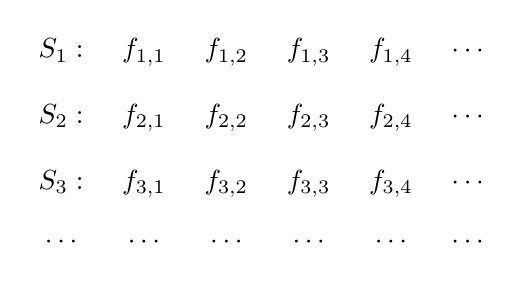
\begin{tikzpicture}
  \matrix (m) [matrix of math nodes, inner sep=2pt, row sep=1em, column sep=1em]
  {
    S_1: & f_{1,1} & f_{1,2} & f_{1,3} & f_{1,4} & \cdots \\
 S_2: & f_{2,1} & f_{2,2} & f_{2,3} & f_{2,4} & \cdots  \\
 S_3: & f_{3,1} & f_{3,2} & f_{3,3} & f_{3,4} & \cdots  \\
 \cdots & \cdots & \cdots & \cdots &  \cdots &\cdots \\
  };
\end{tikzpicture}
\end{center}
并且具有以下性质:

(a) 对于$n=2,3,\cdots,$ $S_n$是$S_{n-1}$的子序列.

(b) 当$k\to\infty$时, $\{f_{n,k}(x_n)\}$收敛.

(c) 在每个序列中, 函数出现的先后顺序是一样的. 换言之, 如果某个函数在$S_1$中位于另一个函数之前, 那么它们在每个$S_n$中都保持同样的位置关系.

现在取对角线上的函数
$$S: f_{1,1},\quad f_{2,2},\quad f_{3,3},\quad f_{4,4},\quad\cdots$$
于是$S$是$S_n$的子序列 (不过可能要去掉$S$的前$n-1$项), 故而当$n\to\infty$时, 序列$\{f_{n,n}(x_i)\}$对每个$x_i\in E$都收敛.

\end{proof}
\begin{theorem}
 如果$K$是紧度量空间, 对于$n=1,2,\cdots$都有$f_n\in\mathscr{C}(K)$, 并且$\{f_n\}$在$K$上一致收敛, 那么$\{f_n\}$在$K$上等度连续.
\end{theorem}
\begin{proof}
  因为$\{f_n\}$在$K$上一致收敛, 那么对于任意给定的$\epsilon>0$, 总存在正整数$N$, 使得当$n>N$时就有
  $$ |f_n(x)-f_N(x)|\leq  ||f_n-f_N||<\epsilon$$
  因为$K$是紧的, 所以$f$在$K$上一致连续, 因此存在$\delta_i>0$, 使得当$d(x,y)<\delta_i$时就有
  $$|f_i(x)-f_i(y)|<\epsilon\quad (1\leq i\leq N)$$
  取$\delta=\min\{\delta_1,\cdots,\delta_N\}$, 就能保证上式对于每个$1\leq i\leq N$都成立.

  另一方面, 如果$n>N$且$d(x,y)<\delta$, 那么
  $$|f_n(x)-f_n(y)|\leq |f_n(x)-f_N(x)|+|f_N(x)-f_N(y)|+|f_N(y)-f_n(y)|<3\epsilon$$
  因此$\{f_n\}$在$K$上等度连续.
\end{proof}
\begin{theorem}\label{thm:th7.12}
  如果$K$是紧度量空间, 对于$n=1,2,\cdots$都有$f_n\in\mathscr{C}(K)$, 并且$\{f_n\}$在$K$上逐点有界而又等度连续, 那么
  \begin{enumerate}[label=(\arabic*)]
  \item $\{f_n\}$在$K$上一致有界;

  \item $\{f_n\}$含有一致收敛的子序列.
  \end{enumerate}
\end{theorem}
\begin{proof}
  (1) 因为$\{f_n\}$在$K$上等度连续, 那么任取$\epsilon>0$, 总能找到某个$\delta>0$, 使得对于每个$n=1,2,\cdots$, 只要$d(x,y)<\delta$就能保证
  $|f_n(x)-f_n(y)|<\epsilon$.

  因为$K$是紧集, 设$V(p,\delta)$是点$p\in K$的半径为$\delta$的邻域, 并且$\bigcup_p V(p,\delta)$形成$K$的一个开覆盖, 那么$K$中存在有限个点$p_1,\cdots,p_r$使得
  $$K\subset V(p_1,\delta)\cup\cdots\cup V(p_r,\delta)$$
  因此每个$x\in K$至少对于一个$p_i$, 可以使得$d(x,p_i)<\delta$, 此时
  $$|f_n(x)-f_n(p_i)|<\epsilon$$
  又因为$\{f_n\}$在$K$上逐点有界, 于是存在$M_i<\infty$使得对于一切$n=1,2,\cdots$都有$|f_n(p_i)|<M_i$. 取$M=\max\{M_1,\cdots,M_r\}$, 那么对于任意$x\in K$, 总有
  $$|f_n(x)|<M+\epsilon$$
  由于$\epsilon$是任意小的, 所以$\{f_n\}$在$K$上一致有界.

  (2) 设$E$是$K$的可数稠密子集, 定理\ref{thm:th7.4}表明存在$\{f_n\}$的一个子序列$\{f_{n_i}\}$使得$\{f_{n_i}(x)\}$关于每个$x\in E$都收敛, 这里将$f_{n_i}$记作$g_i$以简化符号.

  按照(1)部分证明那样选取某个$\delta>0$, 设$V(x,\delta)$是满足$d(x,y)<\delta$且$y\in K$构成的集合. 因为$E$在$K$中稠密, 而$K$是紧集, 那么$E$中存在有限个点$x_1,\cdots,x_m$使得
  \begin{equation}\label{eq7.21}
    K\subset V(x_1,\delta)\cup\cdots\cup V(x_m,\delta)
  \end{equation}
  因为$\{g_i(x)\}$对于每个$x\in E$都收敛, 由Cauchy准则可知存在正整数$N$, 使得
  $$|g_i(x_s)-g_j(x_s)|<\epsilon$$
  其中$i\geq N$, $j\geq N$, $1\leq s \leq m$. 如果$x\in K$, 式(\ref{eq7.21})表明对于某个$s$, 必有$x\in V(x_s,\delta)$, 又因为$g_i\in\mathscr{C}(K)$, 所以对于每个$i$都有
  $$|g_i(x)-g_i(x_s)|<\epsilon$$
  于是当$i\geq N$, $j\geq N$时就能得到
  $$|g_i(x)-g_j(x)|\leq|g_i(x)-g_i(x_s)|+|g_i(x_s)-g_j(x_s)|+|g_j(x_s)-g_j(x)|<3\epsilon$$
  最后由Cauchy准则可知$\{g_i\}$在$K$上一致收敛.

\end{proof}
\begin{example}
设$\{f_n\}$是一致有界的函数序列, 这些函数都在$[a,b]$上Riemann可积, 令
$$F_n(x)=\int_{a}^{x}f_n(t)\dt, \quad a\leq x\leq b$$
那么存在子序列$\{F_{nk}\}$在$[a,b]$上一致收敛.
\end{example}
\begin{proof}
  因为$\{f_n\}$在一致有界, 那么对于一切$n=1,2,\cdots$都有$|f_n(x)|<M$, 其中$x\in[a,b]$. 因为在$[a,b]$上$f_n\in\RR$, 于是
  $$|F_n(x)|\leq\int_{a}^{x}|f_n(t)|\dt<M(b-a)$$
  因此$\{F_n\}$在$[a,b]$上一致有界. 由定理\ref{thm:th6.9}可知, $F_n$在$[a,b]$上一致连续, 因而对于任意$\epsilon>0$, 取$\delta=\epsilon/M$, 那么当$x,y\in [a,b]$且$|x-y|<\delta$时就有
  $$|F_n(x)-F_n(y)|\leq\int_{y}^{x}|f_n(t)|\dt<M|x-y|<\epsilon$$
  因此$\{F_n\}$是等度连续的, 由定理\ref{thm:th7.12}(2)即可证得.
\end{proof}

\section{Stone-Weierstrass定理}
\begin{theorem}[Weierstrass逼近定理]\label{thm:th7.6}
  如果$f$是$[a,b]$的一个复连续函数, 那么存在多项式序列$\{P_n\}$在$[a,b]$上一致收敛于$f$. 特别地, 如果$f$是实函数, 那么$P_n$可以是实多项式.
\end{theorem}
\begin{proof}
  首先假设$f$是定义在[0,1]上的连续函数($[0,1]$的结论可以推广至$[a,b]$), 并且再假定$f(0)=f(1)=0$, 并且区间$[0,1]$外的一切点$x$都满足$f(x)=0$, 因此$f$在整个实直线上一致连续.

  对于$n=1,2,\cdots$, 设
  $$Q_n(x)=c_n(1-x^2)^n$$
  其中$c_n$的选取可以使得
  \begin{equation}\label{eq7.22}
    \int_{-1}^{1}Q_n(x)\dx=1
  \end{equation}
  设函数$\varphi(x)=(1-x^2)^n-1+nx^2$, $\varphi(0)=0$, 并且
  $$\varphi'(x)=2nx[1-(1-x^2)^{n-1}]$$
  在$(0,1)$内为正, 因此
  $$(1-x^2)^n\geq1-nx^2$$
  考虑积分
  \begin{align*}
  \int_{-1}^{1}(1-x^2)^n\dx&=2\int_{0}^{1}(1-x^2)^n\dx\geq 2\int_{0}^{1/\sqrt{n}}(1-x^2)^n\dx \\
  &\geq 2\int_{0}^{1/\sqrt{n}}(1-nx^2)\dx \\
  &=\frac{4}{3\sqrt{n}}>\frac{1}{\sqrt{n}}
  \end{align*}
  那么根据式(\ref{eq7.22})可知
  \begin{equation}\label{eq7.23}
   c_n<\sqrt{n}
  \end{equation}
  对于任意给定的$\delta>0$, 由式(\ref{eq7.23})可知
  \begin{equation}\label{eq7.24}
    Q_n(x)\leq\sqrt{n}(1-\delta^2)^n
  \end{equation}
  其中$\delta\leq|x|\leq1$, 此时$\{Q_n\}$在$[0,1]$上一致收敛于0. 现在令
  $$P_n(x)=\int_{-1}^{1}f(x+t)Q_n(t)\dt, \quad 0\leq x\leq 1$$
  因为当$t<-x$或$t>1-x$时, $f(x+t)=0$. 于是
  \begin{align*}
  P_n(x)&=\int_{-x}^{1-x}f(x+t)Q_n(t)\dt \\
  &=\int_{0}^{1}f(t)Q_n(t-x)\dt
  \end{align*}
  上式积分是关于$x$的多项式, 于是$\{P_n\}$是多项式序列.

  因为$f$在$[0,1]$一致连续, 故而对于任意给定的$\epsilon>0$, 存在$\delta>0$, 对于一切$x,y\in[0,1]$, 只要当$|x-y|<\delta$时就有
  $$|f(x)-f(y)|<\frac{\epsilon}{2}$$
  设$M=\sup |f(x)|$, 根据$Q_n(t)\geq0$, 式(\ref{eq7.22})和(\ref{eq7.24})的事实, 对于一切$0\leq x\leq 1$以及存在充分大的$n$使得
  \begin{align*}
  |P_n(x)-f(x)|&=\left|\int_{-1}^{1}[f(x+t)-f(x)]Q_n(t)\dt \right| \\
  &\leq \int_{-1}^{1}|f(x+t)-f(x)|Q_n(t)\dt \\
  &\leq 2M\int_{-1}^{-\delta}Q_n(t)\dt+\frac{\epsilon}{2}\int_{-\delta}^{\delta}Q_n(t)\dt+2M\int_{\delta}^{1}Q_n(t)\dt \\
  &\leq 4M\sqrt{n}(1-\delta^2)^n+\frac{\epsilon}{2}<\epsilon
  \end{align*}
  也即多项式序列$\{P_n\}$在$[0,1]$上一致收敛于$f$.

  注意, 以上结论是在$f(0)=f(1)=0$的条件下得到, 倘若这一条件不成立, 只需在区间$[0,1]$上构造函数
  $$g(x)=f(x)-f(0)-x[f(1)-f(0)]$$
  显然它满足$g(0)=g(1)=0$, 再将之前的结论用于$g$. 于是存在$g$必然为某个一致收敛的多项式序列的极限函数, 由于$f-g$也是多项式, 因此$f$也是这样.
\end{proof}
\begin{corollary}\label{cor:cor7.1}
在每个闭区间$[-a,a]$上, 必存在实多项式$P_n$的序列, 满足$P_n(0)$, 并且
$$\limn P_n(x)=|x|$$
在$[-a,a]$上一致地成立.
\end{corollary}
\begin{proof}
  由Weierstrass逼近定理, 存在实多项式序列$\{P_n^\ast\}$, 它在$[-a,a]$上一致收敛于$|x|$. 那么对于任意给定的$\epsilon>0$, 存在正整数$N_1$, 使得当$n\geq N_1$且$x\in[-a,a]$时就有
  $$\left|P_n^\ast(x)-|x|\right|<\frac{\epsilon}{2}$$
  令
  $$P_n(x)=P_n^\ast(x)-P_n^\ast(0)$$
  满足$P_n(x)=0$. 又因为$n\to\infty$时, $P_n^\ast(0)\to 0$, 于是存在正整数$N_2$, 使得当$n\geq N_2$时就有
  $$|P_n^\ast(0)|<\frac{\epsilon}{2}$$
  取$N=\max\{N_1,N_2\}$, 可得
  $$\left|P_n^\ast(x)-|x|\right|\leq\left|P_n^\ast(x)-|x|\right|+|P_n^\ast(0)|<\epsilon$$
  其中$n\geq N$且$x\in[-a,a]$.

\end{proof}
\begin{example}
如果$f$在$[0,1]$连续, 并且对于$n=1,2,\cdots$都有
\begin{equation}\label{eq7.34}
  \int_{0}^{1}f(x)x^n\dx=0
\end{equation}
那么在$[0,1]$上$f(x)=0$.
\end{example}
\begin{proof}
  因为函数$f$在$[0,1]$连续, 根据Weierstrass逼近定理可知, 存在多项式$P_n$使得在$[0,1]$上一致地有
  $$\lim_{n\to\infty}P_n(x)=f(x)$$
  于是$fP_n$在$[0,1]$上一致收敛于$f^2$, 因此根据(\ref{eq7.34})可知
  $$\int_{0}^{1}f^2(x)\dx=\limn \int_{0}^{1}f(x)P_n\dx=0$$
  从而$f$在$[0,1]$上恒为$0$.
\end{proof}
\begin{definition}
  集合$E$上的复函数族$\mathscr{A}$为代数, 如果对于一切$f\in\mathscr{A}$, $g\in\mathscr{A}$都有
  \begin{itemize}
   \item $f+g\in\mathscr{A}$;
   \item $fg\in\mathscr{A}$;
   \item 对于任意$c\in\mathbb{C}$, $cf\in\mathscr{A}$.
   \end{itemize}
   换言之, $\mathscr{A}$对于加法, 乘法和数乘是封闭的.
\end{definition}
\begin{definition}
如果对于一切$n=1,2,\cdots,$ 只要$f_n\in\mathscr{A}$, 并且在$E$上$\{f_n\}$一致收敛于$f$, 就能得到$f\in\mathscr{A}$, 那么代数$\mathscr{A}$就是一致闭的 (uniformly closed). 如果$\mathscr{B}$是$\mathscr{A}$内所有一致收敛函数序列的极限函数构成的集合, 那么$\mathscr{B}$是$\mathscr{A}$的一致闭包 (uniformly closure).
\end{definition}
\begin{example}
全体复多项式构成的集合是一个代数. 并且Weierstrass逼近定理可以描述为$[a,b]$上连续函数的集合是$[a,b]$上多项式的集合的一致闭包.
\end{example}
\begin{theorem}\label{thm:th7.7}
  设$\mathscr{B}$是有界函数的代数$\mathscr{A}$的一致闭包, 那么$\mathscr{B}$是一致闭的代数.
\end{theorem}
\begin{proof}
  如果$f\in\mathscr{B}$, $g\in\mathscr{B}$, 那么存在$f_n\in\mathscr{A}$, $g_n\in\mathscr{A}$使得函数序列$\{f_n\}$和$\{g_n\}$一致收敛于$f$, $g$. 因为$f_n$, $g_n$都是有界的, 因此
  $$f_n+g_n\to f+g,\quad f_ng_n\to fg,\quad cf_n\to f$$
  其中$c\in\mathbb{C}$. 由此$f+g\in\mathscr{B}$, $fg\in\mathscr{B}$, $cf\in\mathscr{B}$, 那么$\mathscr{B}$是一个代数, 最后根据定理\ref{thm:th2.5}(1)可知代数$\mathscr{B}$是一致闭的.
\end{proof}
\begin{remark}
直接使用定理\ref{thm:th2.5}只能说明$\mathscr{B}$是闭的, 而不能说明它是一致闭的, 因为后者是针对代数而言的. 因此需要先证明$\mathscr{B}$是代数.
\end{remark}
\begin{definition}\label{def:def7.3}
\begin{itemize}
\item 设$\mathscr{A}$是集合$E$上的函数族, 如果对于任意不同的点$x_1,x_2\in E$, 总存在函数$f\in\mathscr{A}$, 使得$f(x_1)\neq f(x_2)$, 那么就称$\mathscr{A}$能分离$E$的点.

\item 如果对于任意$x\in E$, 总存在$g\in\mathscr{A}$, 使得$g(x)\neq 0$, 就称$\mathscr{A}$不在$E$的点消失.
\end{itemize}
\end{definition}
\begin{example}
所有一元多项式的代数在$\R$上具有定义\ref{def:def7.3}的性质. 然而考虑定义在$[-a,a]$的偶多项式的代数, 它就不能分离$[-a,a]$上的点.
\end{example}
\begin{theorem}\label{thm:th7.8}
  设$\mathscr{A}$是定义在$E$上函数的代数, $\mathscr{A}$既能分离$E$的点又不在$E$的点消失, $x_1$和$x_2$是$E$中不同的两点, $c_1$和$c_2$是两个常数, 那么存在函数$f\in\mathscr{A}$使得
  $$f(x_1)=c_1,\quad f(x_2)=c_2$$
\end{theorem}
\begin{proof}
  以上假设说明, 存在函数$g, h, k \in\mathscr{A}$使得
  $$g(x_1)\neq g(x_2),\quad h(x_1)\neq0, \quad k(x_2)\neq 0$$
  设
  $$u=gk-g(x_1)k,\quad v=gh-g(x_2)h$$
  由于代数$\mathscr{A}$对加法, 乘法和数乘的封闭性可知$u\in\mathscr{A}$, $v\in\mathscr{A}$. 并且还有$u(x_1)=v(x_2)=0$, $u(x_2)\neq 0$, $v(x_1)\neq 0$. 令
  $$f=\frac{c_1v}{v(x_1)}+\frac{c_2u}{u(x_2)}$$
  于是$f(x_1)=c_1$, $f(x_2)=c_2$.


\end{proof}
\begin{theorem}[Stone-Weierstrass定理]
  设$\mathscr{A}$是紧集$K$上实连续函数的代数, $\mathscr{A}$既能分离$K$的点又不在$K$的点消失, 那么$\mathscr{A}$的一致闭包$\mathscr{B}$由$K$上的所有实连续函数构成.
\end{theorem}
\begin{proof}
  证明分为以下四个部分进行.

  \textcolor[rgb]{0.96,0.53,0.14}{Step 1: 如果$f\in\mathscr{B}$, 那么$|f|\in\mathscr{B}$.}

  因为紧集上的连续函数是有界的, 因此设
  \begin{equation}\label{eq7.25}
    a=\sup |f(x)| \quad (x\in K)
  \end{equation}
  对于任意给定的$\epsilon>0$, 由推论\ref{cor:cor7.1}可知存在$c_1,\cdots,c_n$使得对于充分大的$n$就有
  \begin{equation}\label{eq7.26}
   \left|\sum_{i=1}^{n}c_iy^i-|y|\right|<\epsilon, \quad -a\leq y\leq a
  \end{equation}
  由定理\ref{thm:th7.7}可知$\mathscr{B}$是一致闭的代数, 于是函数
  $$g=\sum_{i=1}^{n}c_if^i$$
  满足$g\in\mathscr{B}$. 由式(\ref{eq7.25})和(\ref{eq7.26})即可推出
  $$|g(x)-|f(x)||<\epsilon, \quad x\in K$$
  其中$n\geq N$. 因为$\mathscr{B}$是一致闭的, 因此$|f|\in\mathscr{B}$.

    \textcolor[rgb]{0.96,0.53,0.14}{Step 2: 如果$f\in\mathscr{B}$, $g\in\mathscr{B}$, 那么$\min\{f,g\}\in\mathscr{B}$, $\max\{f,g\}\in\mathscr{B}$.}

    考虑恒等式
    \begin{align*}
    &\max\{f,g\}=\frac{f+g}{2}+\frac{|f-g|}{2} \\
    &\min\{f,g\}=\frac{f+g}{2}-\frac{|f-g|}{2}
    \end{align*}
    根据第一步的结果与代数$\mathscr{B}$的性质可知成立. 重复操作下去还可推知$\max\{f_1,\cdots,f_n\}\in\mathscr{B}$以及$\min\{f_1,\cdots,f_n\}\in\mathscr{B}$成立.

     \textcolor[rgb]{0.96,0.53,0.14}{Step 3: 设$f$是定义在$K$上的实连续函数, 任取一点$x\in K$, 那么对于任意给定的$\epsilon>0$, 存在函数$g_x\in\mathscr{B}$满足$g_x(x)=f(x)$, 并且\begin{equation}\label{eq7.27}
       g_x(t)>f(t)-\epsilon
     \end{equation}
     对一切$t\in K$成立.}

      由于$\mathscr{B}$是$\mathscr{A}$的一致闭包, 故而$\mathscr{A}\subset\mathscr{B}$. 又因为$\mathscr{A}$满足定理\ref{thm:th7.8}的假定, 那么$\mathscr{B}$也满足. 于是对于任意$y\in K$, 总能找到一个函数$h_y\in\mathscr{B}$, 使得
      \begin{equation}\label{eq7.28}
        h_y(x)=f(x),\quad h_y(y)=f(y)
      \end{equation}
      由于$h_y$是$K$上的连续函数, 因此存在包含点$y$的开集$J_y$, 使得
      \begin{equation}\label{eq7.29}
        h_y(t)>f(t)-\epsilon, \quad t\in J_y
      \end{equation}
      又因为$K$是紧集, 故而存在有限的点$y_1,\cdots,y_n$使得
      \begin{equation*}\label{eq7.30}
        K\subset J_{y_1}\cup\cdots\cup J_{y_n}
      \end{equation*}
      取$g_x=\max\{h_{y_1},\cdots,h_{y_n}\}$, 于是由第二步可知$g_x\in\mathscr{B}$, $g_x(x)=f(x)$且满足式(\ref{eq7.27}).

      \textcolor[rgb]{0.96,0.53,0.14}{Step 4: 设$f$是定义在$K$上的实连续函数, 那么对于任意给定的$\epsilon>0$, 存在函数$h\in\mathscr{B}$, 使得$|h_n(x)-f(x)|<\epsilon$.}


      考虑第三步中对任意$x\in K$作出的$g_x(x)=f(x)$, 由于它在$K$上是连续的, 因此存在包含着点$x$的开集$V_x$, 使得
      $$g_x(t)<f(t)+\epsilon,\quad t\in V_x$$
      因为$K$是紧的, 故而存在有限的点$x_1,\cdots,x_m$使得
      $$K\subset V_{x_1}\cup\cdots\cup V_{x_m}$$
      再取$h=\min\{g_{x_1},\cdots,g_{x_n}\}$, 因此有
      \begin{equation}\label{eq7.32}
        h(t)<f(t)+\epsilon, \quad t\in K
      \end{equation}
      并且由第二步知$h\in\mathscr{B}$. 又因为式(\ref{eq7.27})是对一切$x\in K$成立的, 因此
      \begin{equation}\label{eq7.33}
        h(t)>f(t)-\epsilon, \quad t\in K
      \end{equation}
      也成立, 再将式(\ref{eq7.32})和(\ref{eq7.33})结合起来就完成了Step 4的证明.

      因为$\mathscr{B}$是一致闭的, 因此$h$构成的函数序列在$K$上一致收敛于$f\in\mathscr{B}$, 也即$\mathscr{A}$的一致闭包$\mathscr{B}$由$K$上的所有实连续函数构成.


\end{proof}
\begin{remark}
第三步中的式(\ref{eq7.29})只在各邻域$J_{y}$内才成立, 而式(\ref{eq7.27})要求在$K$上成立, 从而需要取$g_x=\max\{h_{y_1},\cdots,h_{y_n}\}$才能做到. 第四步取$h=\min\{g_{x_1},\cdots,g_{x_n}\}$也是同样的道理.
\end{remark}
Stone-Weierstrass定理对于复代数不成立, 除非$\mathscr{A}$是自伴的. 其中, 自伴意味着如果$f\in\mathscr{A}$, 那么它的复共轭$\overbar{f}\in\mathscr{A}$.

\begin{theorem}\label{thm:th7.10}
  设$\mathscr{A}$是定义在紧集$K$上的复连续函数的自伴代数, 并且$\mathscr{A}$既能分离$K$的点又不在$K$的点消失. 那么$\mathscr{A}$的一致闭包$\mathscr{B}$由$K$上的所有复连续函数构成. 也就是说, $\mathscr{A}$在$\mathscr{C}(K)$中稠密.
\end{theorem}
\begin{proof}
  设$\mathscr{A}_{\R}$是$K$上所有属于$\mathscr{A}$的实函数构成的集合. 如果$f\in\mathscr{A}$并且$f=u+\text{i}v$, 其中$u$和$v$是实函数, 那么就有$2u=f+\overbar{f}$. 因为$\mathscr{A}$是自伴的, 因此$u\in\mathscr{A}_{\R}$.

  根据定理\ref{thm:th7.8}, 任取$x_1,x_2\in K$且$x_1\neq x_2$, 那么存在$f\in\mathscr{A}$使得$f(x_1)=1$且$f(x_2)=0$, 进而$u(x_1)=1\neq u(x_2)=0$, 所以$\mathscr{A} _{\R}$能分离$K$的点. 再任取$x\in K$, 存在函数$g\in\mathscr{A}$使得$g(x)\neq 0$, 因此存在$\lambda\in\mathbb{C}$使得$\lambda g(x)>0$, 并且使得$f=\lambda g=u+\text{i}v$, 于是$u(x)>0$, 所以$\mathscr{A}_{\R}$不在$K$的点消失.

  由Stone-Weierstrass定理, $K$上的每个实连续函数在$\mathscr{A}_{\R}$的一致闭包中, 也必然在$\mathscr{B}$中. 于是$u\in\mathscr{B}$且$v\in\mathscr{B}$, 又因为$f=u+\text{i}v$, 所以$f\in\mathscr{B}$.


\end{proof}

\end{document} 